\documentclass[12pt,a4paper]{article}

\usepackage[utf8]{inputenc}		% for special characters
\usepackage[T1]{fontenc}		% for correct use of western european characterfonts
\usepackage{lmodern}
\usepackage{ngerman}			% for german typsetting
\usepackage[authoryear]{natbib}		% author-year citation

\usepackage{microtype}			% for those nasty over/underfull boxes
\usepackage{amsmath}			% for the good math
\usepackage{amsfonts}			% for the good math

\usepackage{hyperref}			% for urls
%\usepackage{pdfpages}			% for including pdfs
\usepackage{graphicx}			% for including graphics
\usepackage{tikz}			% Tikz ist kein Zeichenprogramm!
\usetikzlibrary{arrows,arrows.meta}	% TikZ arrows
\usepackage{booktabs}			% for nicer tables
\usepackage{subfigure}			% for many pictures next to each other
\usepackage[algoruled,linesnumberedhidden,german]{algorithm2e}
\usepackage[labelfont=bf, figurename=Abb.]{caption}	% for bold caption titles
\usepackage{placeins}			% stop floats from jumping to the end of document


%%% new commands %%%

\renewcommand{\abstractname}{Einleitung}

%%% main document %%%

\begin{document}
\pagenumbering{gobble}
\title{Analysetechniken für große Datenbestände}
\author{Alexander Poth \\
	KIT - Karlsruhe Institue of Technology \\
	Information Engineering and Management\\
	\texttt{summary.allekai@gmail.com}}
\date{\today}
\maketitle
\newpage
\begin{abstract}
In unserer heutigen Zeit fallen eine Vielzahl von Daten in allen Bereichen des 
Lebens an. Dies ist der immer effizienteren Datenaufzeichnung und -übermittlung 
geschuldet, z.B. durch RFID-Chips, GPS-Geräten und allerlei Sensoren, die in
unseren Smartphones verbaut sind. Um diese Daten sinnvoll verwerten zu können und
Vorhersagen über unbekannte Variablen treffen zu können, sind Möglichkeiten zur 
Analyse von großen Datenbeständen zu einem der wichtigsten Themen geworden. Ziel 
dieser Zusammenfassung und der zugehörigen Vorlesung ist es, dem Studierenden 
Techniken vorzustellen, die es ihm ermöglichen, \textbf{nichttriviale, implizite 
und potentiell nützliche} Zusammenhänge in Datenbeständen zu finden. Potentiell nützlich 
kann in diesem Kontext bedeuten, dass man keine Ergebnis erhält, die man nicht ohnehin 
schon vorher kannte oder redundant sind. Hierbei ist der Begriff \textit{groß} 
vorsichtig zu benutzen. Die "'Größe"' eines Datenbestandes hängt insbesondere von der
Komplexität der Daten, den Mustern, nach denen man sucht, und der verfügbaren CPU-Power ab.
\end{abstract}
\newpage
\tableofcontents
\newpage
\pagenumbering{arabic}

\section{Statistische Grundlagen}
Zunächst wiederholen wir ein paar Grundlagen aus der Statistik.

\subsection{Beschaffenheit von Daten}
Daten können in verschiedenen Kategorien vorliegen:
\begin{itemize}
	\item \textbf{Nominal}: Hier herrscht keine natürliche Ordnung der
            Werte (z.B. Name, Farbe, ...)
	\item \textbf{Ordinal}: Eine Anordnung ist möglich. Es kann jedoch
            nicht ohne Weiteres eine Metrik angelegt werden (z.B.  ist nicht
            quantifiziert, um wie viel sich groß und gigantisch unterscheiden)
	\item \textbf{Metrisch-diskret}: Es existiert eine abzählbare Anzahl an
            Werten, auf die eine Metrik angewandt werden kann (z.B.
            \({n\in \mathbb{N}\ |\ n \in [0,100]}\))
	\item \textbf{Metrisch-kontinuierlich}: Es existieren überabzählbar viele
            Werte, auf die eine Metrik angewandt werden kann (z.B.
            \({n\in \mathbb{R}\ |\ n \in [0,100]}\))
\end{itemize}
Weiter können die Datensätze auch unterschiedlich komplex sein. Dies kann sich
unter anderem in der \textbf{Dimensionalität} der Daten widerspiegeln. So haben
offensichtlich die Datensätze einer einfachen Namensliste eine geringere
Dimension als die  in den Kundendatenbanken einer großen Firma.

Betrachten wir metrisch skalierte Daten, so gilt für eine Metrik \(d\) und
Domäne \(M\):
\begin{align*}
	&\forall p,q,r \in M:&\\
	\\
	&Symmetrie &d(p,q)=d(q,p)\\
	&Definitheit &d(p,q)=0\Leftrightarrow p = q\\
	&Dreiecksungleichung &d(p,r)\leq d(p,q)+d(q,r)\\
\end{align*}
Eine Metrik bezeichnet hierbei eine Funktion, die den Abstand zweier Punkte in
einem metrischen Raum beschreibt.

\subsection{Einfache deskriptive Statistik}
Im Folgenden betrachten wir einfache Methoden zur Beschreibung von Daten, um
diese besser verstehen zu können. Dafür dienen vor allem so genannte
\textbf{Aggregate}. Sie vereinen \textit{alle Werte} eines Attributes und
berechnen daraus einen \textit{einzigen} skalaren Wert. In Standard-SQL werden
folgende Funktionen verwendet: 
\begin{itemize}
	\item COUNT() - Zählt die Anzahl
	\item SUM() - Bildet die Summe
	\item MIN() - Gibt das Minimum aus
	\item MAX() - Gibt das Maximum aus
	\item AVG() - Berechnet das arithmetische Mittel
\end{itemize}
In spezialisierteren SQL-Versionen gibt es weitere Aggregatsfunktionen (z.B.
für die Bereiche Statistik, Physik, etc.). Manche dieser Aggregate haben den
Vorteil, dass sie sich in ihrer Ausführung parallelisieren lassen, z.B. kann
für die MIN()-Funktion der Datenbestand in kleinere Bestände aufgeteilt werden,
aus denen jeweils das Minimum berechnet wird, woraufhin in einem zweiten
Schritt das Minumim der Hilfsminima berechnet wird.
Aufgrund dieser Eigenschaften lassen sich die Aggregate klassifizieren (\(F\)
bezeichne die Aggregatsfunktion):
\begin{itemize}
	\item \textbf{distributiv}: Formal gibt es eine Funktion \(G\), sodass \(F(\{X_{i,j}\}) = G(\{F(\{X_{i,j}| i = 1, ..., I\}) | j = 1, ..., J\})\) gilt. Auf Deutsch: F wird erst auf Teilmengen ausgeführt, dann G auf der Ergebnismenge. Hierbei ist \(I \in \mathbb{N}\) die Mächtigkeit der Teilmengen und \(J\in\mathbb{N}\) ihre Anzahl (es ist nicht zwingend notwendig, dass alle Teilmengen auch tatsächlich die gleiche Mächtigkeit haben).
	\item \textbf{algebraisch}: Formal gibt es eine Funktion \(G\), die \(M\)-Tupel liefert und \(H\), sodass \(F(\{X_{i,j}\}) = H(\{G(\{X_{i,j}| i = 1, ..., I\}) | j = 1, ..., J\})\) gilt. Auf Deutsch: Die Definition entspricht der distributiver Aggregate, jedoch hat man hier die Freiheit, in der inneren Klammer eine Funktion anzuwenden, die nicht die Ausgangsaggregatfunktion \(F\) ist. So könnte man z.B. AVG() folgendermaßen formalisieren:
	\begin{align*}
		G &: \text{Menge von } \mathbb{R} \rightarrow (\mathbb{R},\mathbb{N}),\ S \mapsto a:= (\sum_{x\in S} x, |S|) \\
		H &: \text{Menge von } (\mathbb{R},\mathbb{N}) \rightarrow \mathbb{R},\ A \mapsto \frac{\sum\nolimits_{a\in A} a.first}{\sum\nolimits_{a\in A}a.second}
	\end{align*}
        Hier werden zunächst alle Teilmengen der Ausgangsmenge auf Tupel,
        bestehend aus der Summe ihrer Elemente und ihrer Mächtigkeit,
        abgebildet. Damit erhält man die Menge aller dieser Tupel \(A\). Diese
        Menge wird daraufhin wieder gemäß der zweiten Zeile auf \(\mathbb{R}\)
        abgebildet.
	\item \textbf{holistisch}: Holistische Aggregate sind all jene, die weder distributiv noch algebraisch sind. Man kann das Problem also nicht in Teilprobleme zerlegen, z.B. bei median() oder häufigsterWert(). \textbf{Definition aus der Vorlesung}: Man kann keine Beschränkung des Speicherbedarfs für Sub-Aggregate angeben.
\end{itemize}
Offensichtlich sind distributive bzw. algebraische Aggregate aufgrund ihrer Parallelisierungsmöglichkeiten effizienter in ihrer Berechnung.

\noindent Eine weitere vorteilhafte Eigenschaft, die eine Aggregatsfunktion haben kann, heißt \textbf{"'Self-Maintainable"'}. Self-Maintainable Aggregatsfunktionen können nach einer Änderung der Daten ihren neuen Wert aus ihrem alten Wert und der Änderung berechnen, z.B. SUM(). Änderungen bedeutet in diesem Fall Einfügen oder Löschen von Daten.

\subsection{Qualifizierung der Tendenz insgesamt}
Als nächstes geht es um Kennzahlen, die etwas über die Tendenz in unseren Daten aussagen. Die bekannteste ist das \textbf{arithmetische Mittel}
\[\bar{x}= \frac{1}{n} \sum_{i=1}^n x_i\ .\]
Dieses kann man auch weiter verfeinern zum \textbf{gewichteten arithmetischen Mittel}
\[\bar{x}_w = \frac{\sum_{i=1}^n w_i x_i}{\sum_{i=1}^n w_i}\ .\]
Anschaulich beschrieben, wird jedes \(x_i\) mit einem prozentualem Wert
multipliziert.
Laut obiger Klassifikation lassen sich diese Kennzahlen als \textit{algebraisch} einstufen. Des Weiteren sind sie nur auf numerische Daten anwendbar.
Wenn es um die Mitte unseres Wertebereiches geht, kann das sogar ein Grundschüler ausrechnen:
\[midrange = \frac{max - min}{2}.\]
Auch \textit{midrange} kann nur auf numerische Daten angewandt werden.

Der \textbf{Median} gibt bei sortierter Anordnung den Wert an, der in der Mitte liegt:
\[
x_{med} = 
\begin{cases}
	x_{\frac{n+1}{2}} &\quad \text{für } n \text{ ungerade,}\\
	\frac{1}{2}(x_{n/2} + x_{n/2+1}) &\quad \text{für } n \text{ gerade.}\
\end{cases}
\]
Der Median lässt sich auf numerische und ordinale Daten anwenden und ist als \textit{holistisch} einzustufen.

Der \textbf{Modus} gibt den Wert an, der im Datenbestand am häufigsten vorkommt. Wenn jeder Wert im Datenbestand nur ein \emph{einziges} Mal auftaucht, ist der Modus nicht definiert. Dies führt bei kontinuierlichen Daten schnell zu Problemen.

\noindent Beim Modus muss beachtet werden, dass evtl. wichtige Informationen über unsere Daten ignoriert werden können, z.B. weitere Peaks bei multimodalen Verteilungen.

\subsection{Quantifizierung der Streuung der Daten}
\textbf{Quantile} sind Lagemaße, die einen Schwellenwert in unseren Daten
beschreiben, d.h. ein bestimmter Anteil ist kleiner als das Quantil, der Rest
ist größer. Besondere Quantile sind die \textbf{Quartile}: Das 0.25-Quartil
\(Q_{0.25}\) bzw. \(Q_1\) gibt den Wert an, für den 25\% der Werte kleiner oder
gleich und 75\% der Werte größer als \(Q_1\) sind. Analog wird
\(Q_{0.75}\) bzw. \(Q_3\) definiert. Es gilt: \(Q_2 = Q_{0.5} = x_{med}\). Mit
diesen Quartilen lässt sich der so genannte \textbf{Inter-Quartils-Abstand}
definieren als \(IQR = Q_3 - Q_1\). Als \textbf{Ausreißer} bezeichnet man
Werte, die mehr als \(1,5 \times IQR\) von \(Q_1\) nach unten oder \(Q_3\)
nach oben abweichen.

Weitere wichtige Streumaße sind \textbf{Stichprobenvarianz} und
\textbf{-abweichung}:
\begin{align*}
	\sigma^{2} &= \frac{1}{n-1}\sum\limits_{i=1}^n (x_i -\bar{x})^2 \\
	\sigma &= \sqrt{\sigma^{2}} \\
\end{align*}
Diese Maße fallen für jede Stichprobe unterschiedlich aus und sollten wie immer
mit Vorsicht interpretiert werden.

\subsection{Boxplots}
\noindent Die Daten in Abb.~\ref{fig:boxplot} sind als Box repräsentiert. Die Ränder der Box sind \(Q_1\) bzw. \(Q_3\), womit die Höhe der Box dem \(IQR\) entspricht. Innerhalb der Box ist \(x_{med}\) explizit eingezeichnet. Das Minimum und Maximum sind als "'whiskers"' eingezeichnet.
\begin{figure}[ht]
	\centering
	\includegraphics[width=0.625\textwidth]{Figures/boxplot}
	\caption[Boxplot Beispiel]{Beispiel eines Boxplots \footnotemark}
	\label{fig:boxplot}
\end{figure}
\footnotetext{2. Foliensatz, S.17, Analysetechniken für große Datenbestände, Prof. Dr.-Ing. Klemens Böhm}

\subsection{Histogramme}
\textbf{Histogramme} zeigen die Häufigkeit, mit der einzelne Werte auftreten.
Falls nahezu bzw. alle Werte unterschiedlich sind, hat man jedoch mit einem
Histogramm nichts gewonnen. Deswegen werden die Daten in Klassen bzw.
"'Buckets"' unterteilt. Dies stellt im Allgemeinen eine recht gute
Approximation dar. Wählt man die Partitionierung derart, dass alle Klassen
gleich breit sind, erhalten wir ein \textit{Equi-Width}-Histogramm,
Abb.~\ref{fig:equiWidth}.

\begin{figure}[ht]
	\centering
	\includegraphics[width=0.625\textwidth]{Figures/equiWidth}
	\caption[Equi-Width Beispiel]{Beispiel eines Equi-Width-Histogramms \footnotemark}
	\label{fig:equiWidth}
\end{figure}
\footnotetext{2. Foliensatz, S.20, Analysetechniken für große Datenbestände, Prof. Dr.-Ing. Klemens Böhm}

\noindent Wählt man jedoch die Klassen so, dass alle gleich viele Elemente enthalten, so ergibt sich ein \textit{Equi-Depth}-Histogramm, Abb.~\ref{fig:equiDepth}.

\begin{figure}[ht]
	\centering
	\includegraphics[width=0.625\textwidth]{Figures/equiDepth}
	\caption[Equi-Width Beispiel]{Beispiel eines Equi-Depth-Histogramms \footnotemark}
	\label{fig:equiDepth}
\end{figure}
\footnotetext{2. Foliensatz, S.21, Analysetechniken für große Datenbestände, Prof. Dr.-Ing. Klemens Böhm}

Probleme ergeben sich für Histogramme bei höher dimensionalen Datenbeständen. In den Beispielen der Abb.~\ref{fig:equiWidth} und~\ref{fig:equiDepth} handelt es sich um 1-dimensionale Daten. Diese können leicht klassiert werden. Wie aber sollen z.B. 4-dimensionale Daten gleichmäßig auf Buckets verteilt werden? Außerdem legt man zu Beginn fest, wie groß die Partitionierung ausfällt, womit bei späteren Schätzungen, die auf diesen Histogrammen basieren, nicht weiter mit der Genauigkeit variiert werden kann. Insgesamt ist die Genauigkeit der Approximation durch ein Histogramm in hohem Maße abhängig von der richtigen Wahl der Partitionierung.

\subsection{Entropie}
Die \textbf{Entropie} einer Menge gibt an, wie zufällig die Daten in ihr verteilt sind, d.h. die Entropie dient als Maß für die Unordnung und ist definiert als
\[
	E(S)=-\sum\limits_{j\in S} p_j \log{p_j}.
\]
Hierbei bezeichnet \(j\) die Klassen in \(S\), \(p_j\) die relative Häufigkeit der Elemente in Klasse \(j\) und \(\log{p_j}\) wird als statistische Signifikanz bezeichnet. Da \(p_j \leq 1 \), gilt \(\log{p_j} \leq 0\), was durch das negative Vorzeichen der Summe aufgehoben wird. Offensichtlich ist die Entropie minimal, wenn alle Werte in einer Klasse liegen, da somit \(p_1 = 1\) wird und sich alle Summanden zu \(0\) ergeben. Im Gegensatz dazu wird die Entropie für eine gegebene Klassenanzahl maximal, wenn \(p_i = p_j,\ \forall i,j\in S\) gilt, die Werte also über alle Klassen gleichverteilt sind. 

An dieser Stelle sei ausdrücklich auf die Relevanz der Entropie sowie der
Erweiterung und Anwendung, die in späteren Kapiteln auftreten hingewiesen.

\subsection{Wahrscheinlichkeitstheorie}
Die Wahrscheinlichkeitstheorie ist zentral für die Datenanalyse, da viele
Algorithmen auf Annahmen probabilistischer Natur über den Datenbestand beruhen.
Ein zentrales Konzept ist der \textit{Wahrscheinlichkeitsraum}, der durch das
3-Tupel \((\Omega, F, P)\) beschrieben wird. Hierbei ist \(\Omega\) die
Ergebnismenge, \(F\subseteq 2^{\Omega}\) der Raum der Ereignisse und \(P\) ist
das Wahrscheinlichkeitsmaß, dass jedem Ereignis einen Wert aus \([0,1]\) zuweist.
\(F\) ist hierbei abgeschlossen unter Komplement und Vereinigung und enthält
das triviale (sichere) und leere (unmögliche) Ereignis. Das
Wahrscheinlichkeitsmaß \(P\) erfüllt die \textit{Axiome von Kolmogorow}:
\begin{align*}
	&\text{(K1) Nichtnegativität}	&\quad P(a)\geq 0\\
	&\text{(K2) Triviales Ereignis}	&\quad P(\Omega) = 1\\
	&\text{(K3) Additivität}	&\quad \text{Für } a\cap b = \emptyset: P(a\cup b) = P(a) + P(b)\\
\end{align*}

\noindent Variablen, deren Wert vom Zufall abhängt, nennen wir ganz kreativ \textbf{Zufallsvariable}. Diese Zufallsvariablen können auch als Abbildung aufgefasst werden. Dabei wird jedem \(\omega \in \Omega\) ein reeller Wert \(x = X(\omega)\) zugewiesen, was auch als \textit{Realisierung} von \(X\) bezeichnet wird. Mit \(X\) können aber auch \textbf{Ereignisse} beschrieben werden, z.B. \(\{X = x\} \text{ oder } \{X \leq x\}\). Man denke anschaulich an das Werfen mit 2 Würfeln, wobei \(X = \text{ Summe der Augen}\).

\begin{figure}[hb]
	\centering
	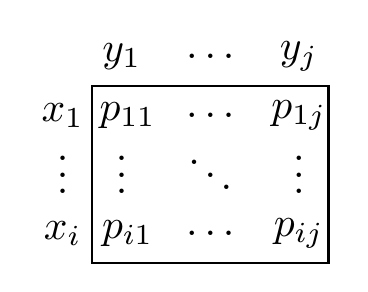
\begin{tikzpicture}[scale=1.5, every node/.style={transform shape}]
	\draw[thick] (0.5,0.5) -- (2.5,0.5) -- (2.5,2) -- (0.5,2) -- cycle;
	\draw (0.25,0.75) node {\(x_i\)};
	\draw (0.25,1.35) node {\(\vdots\)}; 
	\draw (0.25,1.75) node {\(x_1\)}; 
	\draw (0.75,2.25) node {\(y_1\)};
	\draw (1.5,2.25) node {\(\dots\)};
	\draw (2.25,2.25) node {\(y_j\)};
	\draw (0.8,1.75) node {\(p_{11}\)};
	\draw (0.8,0.75) node {\(p_{i1}\)};
	\draw (2.25,0.75) node {\(p_{ij}\)};
	\draw (2.25,1.75) node {\(p_{1j}\)};
	\draw (1.5,1.75) node {\(\dots\)};
	\draw (1.5,0.75) node {\(\dots\)};
	\draw (0.75,1.35) node {\(\vdots\)};
	\draw (2.25,1.35) node {\(\vdots\)};
	\draw (1.5,1.35) node {\(\ddots\)};
\end{tikzpicture}

	\caption[Schema Kontingenztabelle]{Schema einer Kontingenztabelle}
	\label{fig:contingency_ex}
\end{figure}

Multivariate Verteilungen beschreiben die Wahrscheinlichkeitsverteilung einer mehrdimensionalen Zufallsvariable bzw. mehrerer Zufallsvariablen. Zumindest für 2-dimensionale Zufallsvariablen kann die Verteilung in einer \textit{Kontingenztabelle} dargestellt werden, die schematisch in Abb.~\ref{fig:contingency_ex} zu sehen ist. Summiert man die einzelnen Spalten auf, so erhält man die Randverteilung für \(Y\); summiert man die einzelnen Zeilen auf, so erhält man die Randverteilung von \(X\).

Die Zufallsvariablen können aber auch voneinander abhängen. Die Verteilung
einer Zufallsvariable, gegeben den Wert der anderen, nennt man \textbf{bedingte
Verteilung} und wird durch
\[
	P(X=a\ |\ Y=b)=\frac{P(X=a,Y=b)}{P(Y=b)}
\]
beschrieben. Mithilfe der Kontingenztablle lassen sich die Werte des Bruchs direkt ablesen. Falls die Variablen \textbf{unabhängig} voneinander sind, gilt \(P(X) = P(X|Y)\) und \(P(X,Y) = P(X)P(Y)\).

Sei im Folgenden \(X\) eine diskrete Zufallsvariable. Dann bezeichnet \(f(x)=P(X=x)\) für alle \(x\in\mathbb{R}\) die Wahrscheinlichkeitsfunktion von \(X\). Für \(f(x)\) gilt \textit{Nichtnegativität} und es muss \(\sum f(x) = 1\) sein. Würde man diese Funktion plotten, so hätte man im Prinzip ein Stabdiagramm.
Sei \(X\) nun kontinuierlich. Damit ergibt sich die \textit{Wahrscheinlichkeitsdichtefunktion} zu \(P(X\in[a,b])=\int_{a}^{b} f(x)dx\) und auch hier gilt \textit{Nichtnegativität}. Weiter muss \(\int_{-\infty}^{\infty} f(x)dx = 1\) sein.

Der \textbf{Erwartungswert} \(E(X)\) für den diskreten bzw. kontinuierlichen Fall lautet
\begin{align*}
	&E(X)=\sum_{i\geq 1} x_i f(x_i) &E(X) = \int_{-\infty}^{\infty}xf(x)dx.
\end{align*}
Durch den Verschiebungssatz erhalten wir für die \textbf{Varianz} \(Var(X)=E(X^2)-E(X)^2\). Somit ergeben sich für diskrete bzw. kontinuierliche Zufallsvariablen
\begin{align*}
	&Var(X)=\sum_i f(x_i) x_i^2 - (\sum_i f(x_i) \bar{x})^2&Var(X)=\int_{-\infty}^{\infty} x^2f(x)dx - E(X)^2.
\end{align*}

Um Zusammenhänge zwischen den Zufallsvariablen anschaulich darzustellen, gibt es bestimmte Kennzahlen. Zum einen die \textbf{Kovarianz}, die als
\begin{align*}
	Cov(X,Y) &:= E([X-E(X)][Y-E(Y)])\\
	\\
	Cov(X,Y) &= 
		\begin{cases}
		\sum\limits_i \sum\limits_j f(x_i,y_j)(x_i-E(X))(y_j-E(Y)) \hfill X \text{ und } Y \text{ diskret}\\
		\int\limits_{-\infty}^{\infty} \int\limits_{-\infty}^{\infty} f(x,y)(x-E(X))(y-E(Y))dxdy\quad X \text{ und } Y \text{ stetig}\\
		\end{cases}
\end{align*}
definiert ist. Betrachten wir die zweite Gleichung. In einem Koordinatensystem
durch den Punkt \((E(X),E(Y))\) liefern die Werte des ersten und dritten
Quadranten einen positiven Beitrag zur Gesamtsumme, die Werte des zweiten und
vierten Quadranten hingegen negative. Damit ergibt sich, dass die Kovarianz
zwar anzeigen kann, ob die Daten positiv/negativ korreliert sind oder
unabhängig; da sie aber unskaliert ist, lässt sich die Stärke der Korrelation
nicht sinnvoll quantifizieren.
Eine gängige Normierung ergibt sich mittels der Standardabweichung und man erhält den \textbf{Korrelationskoeffizienten} 
\[
	\rho(X,Y) = \frac{Cov(X,Y)}{\sqrt{Var(X)} \sqrt{Var(Y)}}.
\] 
Dieser ist auf \([-1,1]\) normiert, womit sich nun auch die Stärke der Korrelation bewerten lassen kann. Des Weiteren gilt \(Cov(X,X)=Var(X)\).

Für den Fall, dass wir es mit einem Vektor an Zufallsvariablen zu tun haben, kommt die \textbf{Kovarianzmatrix} \(\Sigma\) ins Spiel. Die Kovarianzmatrix als Matrix aller paarweisen Kovarianzen der Elemente des Zufallsvektors enthält Informationen über seine Streuung und über Korrelationen ziwschen seinen Komponenten.
Formal ergibt sich:
\[
	\resizebox{\textwidth}{!}{
		\(\Sigma = (Cov(X_i,X_j))_{i,j = 1\dots n} = 
		\begin{pmatrix}
			Var(X_1) & Cov(X_1,X_2) &\dots & Cov(X_1,X_n)\\
			Cov(X_2,X_1)& Var(X_2) &\dots & Cov(X_2,X_n)\\
			\vdots &\vdots &\ddots &\vdots\\
			Cov(X_n,X_1) & Cov(X_n,X_2) &\dots &Var(X_n)
		\end{pmatrix}\)
	}
\] 

\subsection{Statistische Tests}
Die folgenden statistischen Tests sollen nur soweit vorgestellt werden, wie es nötig ist, sie anwenden zu können.
Für die genauen mathematischen Herleitungen und Zusammenhänge sei auf die entsprechende Fachliteratur verwiesen.

\subsubsection{Chi-Quadrat Unabhängigkeitstest}
\(\chi^{2}\)-Tests bezeichnen zunächst eine ganze Klasse von Tests. Hier wollen wir uns jedoch auf den Unabhängigkeitstest beschränken.
Mit ihm können wir eine Aussage über die Unabhängigkeit zweier Zufallsvariablen
 \(X\) und \(Y\) treffen. Meist liegt eine zu untersuchende Kontingenztabelle
vor. Damit lässt sich der gesamte Test kurz zusammenfassen:
\begin{itemize}
	\item \textbf{Annahmen:} Unabhängige  Stichprobenvariablen \((X_i,Y_i), i = 1,\dots , n\), gruppiert in eine \((k\times m)\)-Kontingenztabelle
	\item \textbf{Hypothese:} \begin{align*}
					&H_0: &P(X=i,Y=j) &= P(X=i) P(Y=j)\ \forall\ i,j\\
					&H_1: &P(X=i,Y=j) &\neq P(X=i) P(Y=j)\\
					& &\text{ für mindestens ein Paar } (i,j).&
				\end{align*}
	\item \textbf{Teststatistik:} \(\chi^2 =\sum\limits_{i=1}^{k}\sum\limits_{j=1}^{m}
					\frac{(h_{ij}-\tilde{h}_{ij})^2}{\tilde{h}_{ij}}\) mit \(\tilde{h}_{ij} = \frac{ h_{i\bullet} h_{\bullet j}}{ n } \)
	\item \textbf{Verteilung unter } \(H_0\): approximativ \(\chi^2((k-1)(m-1))\)
	\item \textbf{Ablehnungsbereich:} \(\chi^2 > \chi_{1-\alpha}^2((k-1)(m-1))\)
\end{itemize}
Der Verlust der Freiheitsgrade tritt durch die Schätzung \(\tilde{h}_{ij}\) auf.
Mit anderen Worten: Ist ein \(\chi^2\)-Wert besonders groß, so kann der
entsprechenden Tabelle die Wahrscheinlichkeit für so einen Wert entnommen werden. Ist dieser sehr
klein, so wird die Nullhypothese verworfen. Bei diesem Test ist zu beachten,
dass der \(\chi^2\)-Wert in hohem Maße von dem Stichprobemumfang \(n\) abhängig ist.

\subsubsection{Kolmogorov-Smirnov-Test}
Dieser Test eignet sich, um Verteilungsannahmen zu prüfen. Es wird angenommen, 
dass die beobachteten Ereignisse bereits sortiert vorliegen. Aus diesen Werten
wird nun die Summenhäufigkeitsfunktion (empirische Verteilungfunktion) \(S\) berechnet,
die nun mit der angenommenen Verteilungsfunktion \(F_0\) verglichen wird. Hierfür werden
an den Stellen \(x_i\) die Differenzen der beiden Funktionen berechnet, also
\(S(x_{i-1})-F(x_i)\) und \(S(x_i)-F(x_i)\). Hierbei ist \(S(x_0):=0\). Man prüft also
die Stärke der Abweichung der angenommenen Funktion von den echten Werten.
Insgesamt ist damit also \(H_0:\ F(x)=F_0(x).\)
Die größte Differenz \(d_{max}\) wird nun mit den Tabellenwerten verglichen. 
Für \(n \leq 35\) liegen diese tabelliert vor, danach muss mit 
\(d_\alpha =\frac{\sqrt{-0,5\ln(\frac{\alpha}{2})}}{\sqrt{n}}\) approximiert werden.

Obwohl nur für eine Zufallsvariable formuliert, lässt sich der Test auch für 2 
Zufallsvariablen durchführen. Dabei gilt nun: \(H_0:\ F(y) = F(x)\).

\subsubsection{Wilcoxon-Mann-Whitney Test}
Auch bekant als Wilcoxon-Rangsummen-Test. Wir fassen kurz zusammen:
\begin{itemize}
	\item \textbf{Annahmen:} \(X_1,\dots,X_n\) unabhängige Wiederholungen von \(X\),\\
				\(Y_1,\dots,Y_m\) unabhängige Wiederholungen von \(Y\),\\
				\(X,Y\) sind unabhängig voneinander,\\
				die Verteilungsfunktionen unterscheiden sich nur durch eine Verschiebung \(a\) voneinander, also \(F_Y(x) = F_X(x-a)\). 
	\item \textbf{Hypothese:} \begin{align}
					&H_0: x_{med}=y_{med} 	&H_1: x_{med}\neq y_{med} \tag{a}\\
					&H_0: x_{med}\leq y_{med} &H_1: x_{med} > y_{med} \tag{b}\\
					&H_0: x_{med}\geq y_{med} &H_1: x_{med} < y_{med} \tag{c}
				\end{align}
	\item \textbf{Teststatistik:} Sortiere die Beobachtungen gepoolt und berechne die Summe der Ränge der
	Elemente der anfangs kleineren Strichprobe. Diese kleinere Stichprobe sei nun \(X\). Die Teststatistik ergibt sich damit als
	\(T_W = \sum\limits_{i=1}^n rg(X_i)\).
	\item \textbf{Ablehnungsbereich:} \begin{align}
						T_W &> w_{1-\alpha /2}(n,m) \text{ oder } T_W < w_{\alpha /2}(n,m) \tag{a}\\
						T_W &> w_{1-\alpha}(n,m) \tag{b}\\
						T_W &< w_{\alpha}(n,m) \tag{c}
					\end{align}
					wobei \(w_{\tilde{\alpha}}\) das \(\tilde{\alpha}\)-Quantil der tabellierten Verteilung bezeichnet.
\end{itemize}
Die genauen kritischen Werte lassen sich aus kombinatorischen Überlegungen 
berechnen. Diese werden jedoch schnell sehr mühselig zu berechnen, wodurch 
die Nutzung der Approximation durch
\[
	W_{n,m} \approx N \left( \frac{n(m+n+1)}{2}, \frac{nm(n+m+1)}{12} \right)
\]
ratsam ist. Die Idee, die hinter diesem Test steckt, ist, dass bei Gültigkeit
der Nullhypothese die Werte der \(X\)- und \(Y\)-Stichproben gut durchmischt
sein sollten, d.h. keine der beiden Stichproben zeigt im Verhältnis zur anderen
eine Tendenz zu besonders großen bzw. kleinen Werten. Der Test stellt nicht direkt
eine Gleichheit von zwei Verteilungen fest, sondern will lediglich eine Aussage über
die Mediane von \(X\) und \(Y\) treffen.

\subsubsection{Bernoulli-Experiment}
Sei \(n\) die Anzahl unserer Datenobjekte,
also die Anzahl der Versuche; \(p\) beschreibe nun die Erfolgswahrscheinlichkeit
eines einzelnen Experiments und \(S\) sei die Anzahl der erfolgreichen Experimente.
Damit ergibt sich als beobachtete Erfolgsquote \(f=\frac{S}{n}\). Ohne
Herleitung ist der Erwartungswert \(E(f) = p\) und die Varianz \(Var(f)= \frac{p(1-p)}{n}\).
Im Allgemeinen ist es das Ziel, \(p\) zu bestimmen, da dieses meist unbekannt ist.
Oft ist jedoch eher die Frage interessant, wie die Grenzen \(z\) gewählt werden
müssen, sodass 
\[
	P(-z \leq f \leq z) = c
\]
gilt. Normiert man \(f\), so kann man die Werte für \(z\) aus der Tabelle
der Standardnormalverteilung ablesen. Es ergibt sich
\[
	P(-z < \frac{f-p}{\sqrt{p(1-p)n}} < z) = c ,
\]
was nun nach Umformung nach \(p\) die Grenzen für dieses liefert. Hierbei
muss man beachten, dass \(n\) groß sein muss. Wie groß, da scheiden sich
die Geister.

Wiederholt man nun ein Bernoulli-Experiment beliebig oft, so lässt sich auch
die Wahrscheinlichkeit für eine bestimmte Folge von Ausgängen berechnen. Formal
ergibt sich
\[
	\prod\limits_{i=1}^{n} p^{y_i} (1-p)^{1-y_i}
\]
wobei \(y_i\) den Ausgang des \(i\)-ten Experiments bezeichnet und nur die Werte
\(0\) oder \(1\) annehmen kann. Das bedeutet, dass im Produkt am Ende pro Faktor
entweder \(p\) oder \(1-p\) steht. Da \(p\) jeodch meist unbekannt ist, kann man
stattdessen \(E(p) = \frac{\sum y_i}{n}\) verwenden, was im Prinzip ein 
\textit{Maximum-Likelihood-Schätzer} für \(p\) ist. Und da es egal ist, ob man,
wenn man \(p\) maximieren möchte, den obigen Ausdruck selbst, oder den Logarithmus
davon berechnet, ergibt sich stattdessen die \textbf{Log-Likelihood-Funktion}
\[
    \sum\limits_{i_1}^n (y_i \log{p} + (1-y_i)\log(1-p)).
\]
Auch hier gilt, dass pro Summand vom inneren Term nur ein Summand übrig bleibt.
Die Log-Likelihood-Funktion bietet den Vorteil, dass man nicht so viele Produkte
berechenen muss, und das aufsummieren schneller geht.


\subsection{Datenreduktion}
Da wir in unserer heutigen Zeit ein Unmenge an Daten sammeln, ist es zum Teil nicht
mehr möglich, die Daten roh zu verarbeiten bzw. zu analysieren. Deswegen kann es
nötig werden, die Daten irgendwie zu verkleinern. Die grundsätzlichen Methoden
hierfür sind
\begin{itemize}
	\item \textbf{Numerosity Reduction} - Die Reduzierung der Anzahl der Datenobjekte
	\item \textbf{Dimensionality Reduction} - Die Reduzierung der Anzahl der Attribute
	\item \textbf{Diskretisierung} - Die Vergröberung der Attributwerte
\end{itemize}
Im Folgenden werden wir die einzelnen Methoden etwas genauer betrachten.

\subsubsection{Numerosity Reduction}
Hier muss grundlegend zwischen zwei Arten von Verfahren unterschieden werden. Die
einen sind \textit{parametrische} Verfahren, die anderen \textit{nichtparametrische}.
Beim parametrischen Verfahren werden zunächst statistische Tests auf den Datenbestand
(oder nur einen Teil davon) angewandt, welche die Art der Verteilung liefern. Kann
man nun annehmen, dass die Verteilung des Datenbestandes der einer bekannten Verteilung
folgt, so braucht man sich lediglich die Parameter der bekannten Verteilung (z.B 
Mittelwert und Varianz bei einer Normalverteilung) merken. Dass dies eine enorme
Reduktion darstellt ist offensichtlich.

Die nichtparametrischen Verfahren treffen zunächst keinerlei Annahme über die
Verteilung der Werte des Datenbestandes. Methoden zur Reduktion umfassen hier
\textit{Histogramme, Sampling} und \textit{Clustering}. Histogramme wurden bereits
weiter oben besprochen. \textbf{Sampling} bedeutet, dass nur ein möglichst 
repräsentativer Ausschnitt des Datenbestandes verwendet wird. Dies kann die 
Komplexität mancher Analysealgorithmen erheblich reduzieren. \textbf{Clustering}
ist relativ selbsterklärend, setzt jedoch voraus, dass sich die Daten in Cluster
aufteilen lassen. So kann man jedes Cluster am Ende für sich betrachten und muss
nur die relevanten Clustereigenschaften, z.B. Anzahl der enthaltenen Datenobjekte,
lienare Summe, square sum, etc., speichern, aus denen man dann Werte wie die
Clustermitte oder -radius berechnen kann. Auf diese Methode wird in einem späteren
Kapitel näher eingegangen.

\subsubsection{Dimensionality Reduction}
\textbf{Feature Selection:} Man kann Attribute, die unnötig sind, auch einfach
weglassen. Dies setzt jedoch ein Wissen über die spzifische Domäne voraus. Hat
man dieses Wissen nicht, müssen andere Maßstäbe angesetzt werden, z.B. welche 
Attribute lassen sich relativ gut mit anderen Anttriubutwerten vorhersagen,
sprich wo liegt eine Abhängigkeit vor? Da es insgesamt \(2^d\) mögliche
Teilmengen von Attributen gibt (\(d\) ist die Mächtigkeit der Domäne), 
können wir die Lösung oft nicht direkt explizit ausrechenen. Hier
müssen Heuristiken zur Auswahl der Dimensionen angewandt werden, z.B. wird zuerst die
\textit{Vorhersagekraft} jedes Attributs ermittelt und nur die besten Attribute
werden behalten, oder es erfolgt eine schrittweise Auswahl der miteinander am vorhersagekräftigsten
Attribute bis man genügend hat; analog kann auch eine schrittweise Eliminierung der am
wenigsten nützlichen Attribute erfolgen. Dies entspricht eine Top-Down bzw.
Bottom-Up Ansatz. Denkbar ist natürlich auch eine Kombination der beiden
Verfahren, d.h. in jeder Iteration wird sowohl ein neues Attribut hinzugefügt,
also auch ein altes entfernt. Dies kann insbesondere im Bereich der Regression
ein nützliches Verfahren bei der Auswahl der Regressoren sein. Auf dieses Weise
kann auch Multikollinearität in gewisser Weise berücksichtigt werden. Für eine
tiefergehende Betrachtung der Herausforderungen, die sich bei der Feature
Selection ergeben, sei auf einschlägige Ökonometrie Veranstaltungen und
entsprechende Literatur verwiesen.

\textbf{Hauptachsentransformation:} Auch Singulärwertzerlegung genannt, oder auf 
englisch Principal Component Analysis, Singular Value Decomposition oder Latent 
Semantic Indexing. Gegeben einem Datenbestand von \(N\) \(k\)-dimensionalen 
Datenobjekten: Finde nun \(c\leq k\) orthogonale Vektoren, die den Datenbestand
am besten repräsentieren. Lägen beispielsweise alle Datenpunkte im \(\mathbb{R}^2\)
auf einer Geraden durch den Ursprung, so würde es sich doch anbieten, die Gerade
als neue Hauptachse zu nehmen und die andere Achse wegzulassen, da mit der Geraden
bereits alle Datenobjekte beschrieben werden. Dieser Fall ist natürlich komplett
konstruiert; würden sich aber die Werte relativ nah um eine Gerade herum verteilen,
so würde diese Gerade schon ausreichen.

Diese eher graphische Darstellung kann mit der Singulärwertzerlegung auch für
Matrizen und höher-dimensionale Probleme angewandt werden. Da SVD eine äußerst
wichtige Methode zur Datenreduktion und auch Analyse ist, wollen wir hier mit 
einem extensiveren Beispiel arbeiten, als es in der Vorlesung gegeben ist.

% latex table generated in R 3.2.3 by xtable 1.8-2 package
% Sun Nov  6 23:03:19 2016
\begin{table}[th]
	\centering
	\caption{Ein Beispiel Datenbestand mit Filmbewertungen von verschieden Personen.}
	\label{tab:svd_example}
	\resizebox{\textwidth}{!}{
\begin{tabular}{rrrrrrr}
  \hline
 & Avengers & Dr.Strange & Ant.Man & Batman & Superman & Watchmen \\ 
  \hline
Tony &  10 &   9 &   8 &   1 &   0 &   0 \\ 
  Thor &  10 &  10 &   7 &   0 &   0 &   1 \\ 
  Stephen &   8 &  10 &   8 &   0 &   0 &   0 \\ 
  Scott &  10 &   9 &  10 &   2 &   0 &   0 \\ 
  Bruce &   1 &   0 &   0 &  10 &   9 &   8 \\ 
  Clark &   2 &   0 &   0 &   9 &  10 &   9 \\ 
  Dr. Manhatten &   1 &   0 &   0 &   7 &   7 &  10 \\ 
  Rorschach &   0 &   0 &   0 &   9 &   8 &  10 \\ 
   \hline
\end{tabular}
}
\end{table}


Betrachten wir also zunächst Tablle~\ref{tab:svd_example}. Man kann durchaus vermuten,
dass die jeweiligen Superhelden die Filme aus ihrem eigenen Universum besser bewerten.
Diese Werte lassen sich auch in Form einer Matrix \(A\) aufschreiben

\begin{align*}
	A = % latex table generated in R 3.2.3 by xtable 1.8-2 package
% Sun Nov  6 23:25:21 2016
\begin{bmatrix}{}
   10 &   9 &   8 &   1 &   0 &   0 \\ 
   10 &  10 &   7 &   0 &   0 &   1 \\ 
    8 &  10 &   8 &   0 &   0 &   0 \\ 
   10 &   9 &  10 &   2 &   0 &   0 \\ 
    1 &   0 &   0 &  10 &   9 &   8 \\ 
    2 &   0 &   0 &   9 &  10 &   9 \\ 
    1 &   0 &   0 &   7 &   7 &  10 \\ 
    0 &   0 &   0 &   9 &   8 &  10 \\ 
  \end{bmatrix}

\end{align*}
Für diese \(m\times n\)-Matrix \(A\) mit Rang \(r\) gilt nun, dass sie sich immer 
Zerlegen lässt in
\[
	A = U\Sigma V^*
\]
wobei \(U\) eine \textbf{unitäre} \(m\times m\)-Matrix\footnote{\textbf{Unitär} bedeutet,
dass \(U^{H}*U = I\), wobei \(U^{H}\) die Adjungierte ist.}, \(\Sigma\) eine 
reelle \(m\times n\)-Matrix und \(V^*\) die \textbf{Adjungierte}\footnote{
\textbf{Adjungiert} ist die komplex-kunjugierte Transponierte einer Matrix (die Reihenfolge der
Operationen ist hierbei unerheblich).} einer
\textbf{unitären} \(n\times n\) Matrix \(V\) ist. \(\Sigma\) hat die spezielle Form, dass
sich auf den ersten \(r\) Diagonaleneinträgen die \textbf{Singulärwerte}\footnote{Singulärwerte
können als Streckung der Vektoren betrachtet werden.} von \(A\)
befinden, die auch durch \(A\) eindeutig bestimmt sind. Alle anderen Werte von
\(\Sigma\) sind \(0\). Die Spaltenvektoren von \(U\) heißen \textbf{Links-Singulärvektoren}
und die Spaltenvektoren von \(V\) heißen \textbf{Rechts-Singulärvektoren}.
Das scheint erstmal wieder schrecklich viel Mathe zu werden. Es sollen aber im
Endeffekt zunächst nur die Begriffe hängen bleiben. Fahren wir mit dem Anschaulichen
fort. Lassen wir uns die Werte aus Tabelle~\ref{tab:svd_example} in einer Heatmap
plotten, ergibt sich Abb.~\ref{fig:original_data}.

\begin{figure}[!th]
	\center
	\includegraphics[width=0.5\textwidth]{Figures/original_data}
	\caption{Die Rohdaten als Heatmap.}
	\label{fig:original_data}
\end{figure}

Aus dieser Heatmap lässt sich einfach erkennen, dass es offensichtlich zwei
Cluster gibt, nämlich die Marvel-Fans und die DC-Fans, welche die jeweils anderen
hassen. Es gibt also zwei "'Konzepte"', die den Datenbestand prägen. Damit kann
es also durchaus interessant sein, die Anzahl der betrachteten Dimensionen auf ein
Minimum zu reduzieren, ohne einen großen Informationsverlust in Kauf nehmen zu müssen.
Hierfür ist die Singulärwertzerlegung zuständig. Wendet man in \textit{R} auf
obigen Datenbestand die \textit{svd()}-Funktion an, so ergibt sich

\begin{align*}
	U &= % latex table generated in R 3.2.3 by xtable 1.8-2 package
% Mon Nov  7 00:01:39 2016
\begin{bmatrix}{}
  -0.41 & 0.28 & -0.11 & -0.14 & -0.31 & 0.22 \\ 
  -0.41 & 0.28 & 0.43 & -0.44 & -0.07 & 0.36 \\ 
  -0.38 & 0.29 & 0.16 & 0.09 & 0.75 & -0.36 \\ 
  -0.44 & 0.29 & -0.43 & 0.50 & -0.31 & -0.19 \\ 
  -0.29 & -0.41 & -0.47 & -0.14 & 0.26 & 0.46 \\ 
  -0.32 & -0.42 & -0.18 & -0.51 & -0.11 & -0.59 \\ 
  -0.26 & -0.37 & 0.55 & 0.26 & -0.35 & -0.16 \\ 
  -0.28 & -0.43 & 0.18 & 0.43 & 0.21 & 0.28 \\ 
  \end{bmatrix}
\\
	\Sigma &= % latex table generated in R 3.2.3 by xtable 1.8-2 package
% Mon Nov  7 00:01:39 2016
\begin{bmatrix}{}
  32.43 & 0.00 & 0.00 & 0.00 & 0.00 & 0.00 \\ 
  0.00 & 29.87 & 0.00 & 0.00 & 0.00 & 0.00 \\ 
  0.00 & 0.00 & 3.36 & 0.00 & 0.00 & 0.00 \\ 
  0.00 & 0.00 & 0.00 & 2.32 & 0.00 & 0.00 \\ 
  0.00 & 0.00 & 0.00 & 0.00 & 1.82 & 0.00 \\ 
  0.00 & 0.00 & 0.00 & 0.00 & 0.00 & 1.01 \\ 
  \end{bmatrix}
\\
	V &= % latex table generated in R 3.2.3 by xtable 1.8-2 package
% Mon Nov  7 00:00:14 2016
\begin{bmatrix}{}
  -0.52 & 0.31 & -0.04 & -0.44 & -0.65 & 0.13 \\ 
  -0.48 & 0.37 & 0.30 & -0.13 & 0.68 & 0.26 \\ 
  -0.42 & 0.32 & -0.27 & 0.64 & -0.03 & -0.49 \\ 
  -0.35 & -0.45 & -0.53 & 0.22 & 0.06 & 0.58 \\ 
  -0.30 & -0.47 & -0.21 & -0.49 & 0.25 & -0.58 \\ 
  -0.34 & -0.50 & 0.71 & 0.30 & -0.22 & -0.03 \\ 
  \end{bmatrix}

\end{align*}

Wenn wir uns nun \(\Sigma\) etwas näher anschauen, stellen wir fest, dass es
zwei große Werte gibt, nämlich \(\sigma_1\) und \(\sigma_2\), und die anderen
Werte eher schwach ausfallen. Dies zeigt uns, dass die einzigen wirklich aussagekräftigen
Werte \(\sigma_1\) und \(\sigma_2\) sind und wir die übrigen vernachlässigen
können. Dies geschieht, indem alle anderen \(\sigma\) gleich \(0\) gesetzt werden,
wodurch bei der Multiplikation \(U\Sigma V^*\) die rechten Spalten von \(U\) und die
unteren Zeilen von \(V^*\) effektiv wegfallen.
Am Ende kommt eine Art Approxmination \(\tilde{A}\) von \(A\) heraus mit
\[
	\tilde{A} = % latex table generated in R 3.2.3 by xtable 1.8-2 package
% Mon Nov  7 01:11:22 2016
\begin{bmatrix}{}
  9.45 & 9.39 & 8.20 & 0.78 & 0.03 & 0.25 \\ 
  9.47 & 9.42 & 8.22 & 0.79 & 0.04 & 0.26 \\ 
  9.04 & 9.03 & 7.88 & 0.37 & -0.34 & -0.16 \\ 
  10.12 & 10.03 & 8.75 & 1.11 & 0.30 & 0.56 \\ 
  1.04 & -0.01 & 0.02 & 8.92 & 8.66 & 9.34 \\ 
  1.40 & 0.31 & 0.29 & 9.30 & 9.00 & 9.71 \\ 
  0.94 & -0.00 & 0.02 & 7.99 & 7.75 & 8.36 \\ 
  0.67 & -0.38 & -0.31 & 8.92 & 8.69 & 9.36 \\ 
  \end{bmatrix}

\]
Wie man sehen kann, sind die Werte dieser Approximation relativ nahe an den
echten Werten von \(A\) dran.

\begin{figure}[!th]
	\center
	\includegraphics[width=0.5\textwidth]{Figures/reduced_data}
	\caption{Die Heatmap für die Approximation mit reduzierten Daten.}
	\label{fig:reduced_data}
\end{figure}

Die Heatmap in Bild~\ref{fig:reduced_data} zeigt, dass durch die Singulärwertzerlegung
die Struktur der Daten weitestgehend erhalten geblieben ist.

Es sei an dieser Stelle ein Wort der Warnung gegeben: Sollten weitere Datensätze
hinzukommen, die sich nicht so einfach den einzelnen Clustern zuordnen lassen,
wie z.B. die Gottheiten aus Lovecrafts Geschichten, die weder an Marvel noch an DC
besonderen Gefallen finden, so wird die Interpretation der erhaltenen Matrizen
sehr schnell schwierig und die Werte für die Singulärwerte sind auch weitaus weniger
eindeutig. Es ist also im Allgemeinen nicht so einfach, passende Werte zu finden,
die die Struktur des Datenbestanden treffend wiedergeben.

\textbf{Nachreichung:} Dieser Abschnitt über SVD ist vor allem als
Visualisierung zu verstehen. Die Darstellung ist schwer an
\url{https://www.youtube.com/watch?v=P5mlg91as1c} angelehnt. 
Die Mathematik dahinter ist für die Klausur
irrelevant und gerade für Informationswirte nicht unbedingt Teil des mathematischen
Curriculums. Wer sich näher mit diesem Thema befassen möchte, sei auf diverse
Vorlesungen auf YouTube verwiesen oder auch das eine oder andere Mathematik
Lehrbuch. Für die Klausur ist es zum einen unwahrscheinlich, dass dieses Thema
allzu genau abgefragt wird, und zum anderen dürfte es bereits reichen, die
Dimensionen der Matrizen und wie so miteinander verrechnet werden zu kennen.
Die Länge der Darstellung dieses für die Klausur nur begrenzt relevanten Themas
rührt aus der Lust der Autors, mit \texttt{R} ein wenig herumspielen zu wollen.
Der Fokus sollte beim Lernen folglich auf anderen Kapiteln liegen.

\subsubsection{Diskretisierung}
Okay, wir halten uns kurz.  \textbf{Entropiebasierte Diskretisierung:} Wir teilen
unsere Attributmenge \(S\) in kleinere Partitionierungen auf. Wo genau wir aber
die Intervallgrenzen am besten setzen, verrät uns die \textbf{Entropie des Splits}:
\[
	Entropie_{Split}(S,T) = \frac{|S_1|}{|S|} Entropie(S_1) +
	\frac{|S_2|}{|S|} Entropie(S_2)
\]
Hierbei ist \(T\) der Schwellenwert für den Split. Diesen gilt es effizient zu wählen.
Natürlich lässt sich das auch für mehr als 2 Partitionen implementieren. Optimal ist unsere
Partitionierung, wenn obige Funktion minimiert wird. Die Berechnung wird rekursiv
durchgeführt, bis irgendein Abbruchkriterium erfüllt ist.

Grundsätzlich kann man zwischen \textit{top-down} und \textit{bottom-up} Verfahren
bei der Diskretisierung unterscheiden, die dann entweder Split- oder Merge-basiert
arbeiten. Hat man z.B. bereits eine Partitionierung kleinen Intervalls, hat jedoch
zu viele Partitionen, ist es sinnvoll, gut zusammenpassende Intervalle zu einem
größere zusammenzufassen. Ein passender Algorithmus wäre der s.g. \textbf{Chi-Merge},
der darauf beruht, dass der \(\chi^2\)-Test auf den einzelnen Intervallen 
Zusammenhänge zwischen den Verteilungen der Intervallnachbarn aufdeckt, und diese
bei Übereinstimmung zusammenfügt. Dieser Algorithmus läuft ebenfalls so lange,
bis irgendein Abbruchkriterium erfüllt ist. Wir werden nicht näher auf ihn
eingehen, \texttt{R} und andere Statistik Software können das auch so berechnen.

\newpage
\section{Informatik Grundlagen}

\subsection{Indizierung allgemein}
Bei großen Datenbeständen ist es nicht mehr möglich, die gesamten Daten in den
Arbeitsspeicher unseres Rechners zu laden. Ein schneller Zugriff und eine
effiziente Verarbeitung der Daten ist jedoch nur
vom Arbeitsspeicher aus möglich, wodurch die Daten erst vom Hauptspeicher (z.B. Disk,
HDD, etc.) in den RAM geladen werden müssen, was eine relativ teure Operation ist.
Kommt es hier zu Verzögerungen, so bezeichnet man diese als \textit{Zugriffslücken}.

Daten im Hauptspeicher liegen zumeist nicht als einzelne Objekte vor, sondern als
ganze \textit{Seiten}. Will man nun auf ein Objekt \(a\) auf Seite \(A\) zugreifen,
so muss die gesamte Seite mit allen ihren enthaltenen Elementen mit in den RAM geladen
werden.

\begin{figure}[ht]
	\centering
	\includegraphics[width=0.75\textwidth]{Figures/index_example}
	\caption[Indizierung Beispiel]{Beispiel für Indizierung eines Seitenweise angeordneten
		Datenbestandes\footnotemark}
	\label{fig:index_example}
\end{figure}
\footnotetext{3. Foliensatz, S.3, Analysetechniken für große Datenbestände, Prof. Dr.-Ing.
Klemens Böhm}

Dies kann nun ausgenutzt werden, um den Zugriff auf die Daten zu vereinfachen. Betrachten
wir das Beispiel in Bild~\ref{fig:index_example}. Würde man hier z.B. alle Leute
mit einem Notendurchschnitt besser als \(3.6\) ausgeben wollen, müssten aufgrund der
fehlenden Sortierung alle Seiten einzeln in den Arbeitsspeicher geladen werden,
um sich die richtigen Kandidaten heraussuchen zu können; das Problem steigt also
linear mit der Anzahl der Seiten. Liegt hingegen ein
\textbf{Index} vor, hier in Form eines Suchbaumes, so kann die Suche erheblich
vereinfacht werden. Dieser Baum ist dahingehend zu verstehen, dass der erste
Eintrag eines Tupels die Note bezeichnet, nach welcher der Index aufgebaut ist,
und der zweite Eintrag gibt die Seite und die Position auf der Seite des Datensatzes
an. Sucht man nun hier nach allen Leuten, mit einem Notenschnitt besser als \(3.6\),
so erkennt man leicht, dass wir im Baum einfach nach links absteigen müssen. Damit
erhalten wir bereits alle Seiten, die wir in unseren Arbeitsspeicher laden müssen.
Ein effizienteres Beispiel wäre es, wenn wir direkt nach einer bestimmen Note fragen.
Würden wir uns also für den größten Streber interessieren, so müssten wir im Baum
lediglich nach links absteigen und den ersten Eintrag betrachten. Dieser liefert uns,
dass auf Seite 2 an Stelle 3 der Streber \#1 steht. Ohne Index hätten wir alle
Seiten in den RAM laden müssen, um sicher zu gehen, dass nicht auf der letzten
Seite jemand mit einer \(1.0\) auftaucht.

Diese Indizierung ist natürlich auch für \textbf{mehrere Attribute} möglich.
Oben kommt die Note \(3,8\) mehrfach vor. Sortieren wir zusätzlich auch nach dem
Namen, erhalten wir eine eindeutigere Indizierung. Es gilt zu beachten, dass
eine Sortierung \((gpa, name)\) im Allgemeinen \textbf{nicht} \((name, gpa)\)
gleicht.

\subsection{Räumliche Indexstrukturen}
\subsubsection{Normalisierung}
Betrachten wir nun Datenbestände mit mehreren Dimensionen. Möchte man hier die
Ähnlichkeit von zwei Datenpunkten bestimmen, so wäre ein naiver Ansatz, einfach
die Distanz zwischen den beiden Punkten im \(n\)-dimensionalen Raum zu berechnen.
Ein Problem ergibt sich jedoch daraus, dass mit der einfachen Berechnung des Abstandes
zweier Punkte der sich ergebende Wert mit der Anzahl der Dimensionen automatisch
mitwächst. Deswegen ist eine Normalisierung nötig. Im zwei-dimensionalen Raum mit
jeweils unterschiedlichen Einheiten würde dies mittels
\[
	a_i = \frac{v_i - min\ v_j}{max\ v_j - min\ v_j}
\]
geschehen, wobei \(v_i\) ein Wert aus dem betrachteten Tupel ist und \(v_j\)
ein Wert aus dem Wertebereich von \(v_i\) ist. Beispielhaft möge \(v_i\) für
das Alter einer Person stehen. Wir begrenzen den Wertebereich von \(v_i\) auf
\([0,\ 120]\). Damit ergeben sich die min / max Werte zu 0 bzw. 120. 

Diese Normierung trägt zwar den Unterschieden in den Einheiten der Dimensionen
Rechnung (z.B. Alter und Einkommen), jedoch noch nicht der Anzahl der Dimensionen.
Würde man nun einfach den Abstand der Punkte berechnen, ergäbe sich mit
\[
	d(x_1, x_2) = \sum\limits_{i\in D} |x_{1,i} - x_{2,i}|
\]
die sogenannte \textit{Manhatten Distance}. Mit dieser Formel ist die Abhängigkeit
des Abstands von den Dimensionen schnell ersichtlich.
Eine höhere Dimensionenzahl führt zu einer größeren Summe. Da die Summanden als
Beträge definiert sind, ergibt sich eine monoton wachsende Folge in Abhängigkeit der
Dimensionalität der Daten. Um diese nun auch sinnvoll zu normieren, gibt
es die \textbf{Manhatten Segmental Distance} mit
\[
	d_D(x_1, x_2) = \frac{\sum\limits_{i\in D} |x_{1,i} - x_{2,i}|}{|D|}
\]
wobei \(|D|\) die Anzahl der Dimensionen ist.

\subsubsection{k-dimensionale Bäume}
Das Konzept von kd-Bäumen ist einfach erklärt. Man nehme eine Dimension und suche
sich den Punkt, bei welchem die Hälfte der Datensätze jeweils auf beide Seiten
verteilt ist. Nun nehme man die nächste Dimension, und wiederhole das Ganze. Dieses
Spiel wird so lange getrieben, bis man entweder jeden Punkt eindeutig durch
einen Pfad beschrieben hat, oder in jedem Blatt nur noch ein gewisse (geringe) 
Anzahl an Elementen liegt. Auf diese Weise kann man Punkte durch Traversieren
des Baumes sehr leicht auffinden. Auch sind Bereichsanfragen möglich. 
Im 2D-Raum würde dadurch eine Art "'Raster"' entstehen.
\textit{Bereichsanfragen} sind möglich, indem man prüft, ob der Raum, den man abfragt,
eine Überlappung mit dem Split des aktuellen Knotens hat, oder nicht. Falls
der Bereich nur in eine Hälfte des Splits fällt, dann kann man einfach in diesen Teilbaum
absteigen und den anderen Teilbaum vernachlässigen. Fällt ein Split jedoch
in den Bereich der Anfrage, so muss man in beide Teilbäume absteigen, um alle
Elemente in diesem Bereich finden zu können.
Die \textit{Nächster Nachbar Anfragen} haben den Vorteil, dass nicht jeder Datenpunkt
einzeln verglichen wird, sondern nur die von bestimmten Zonen, die durch den
kd-Baum gegeben sind. In Algorithmus~\ref{alg:NN} ist ein beispielhafter Algorithmus
für eine NN-Anfrage mit einem kDB-Baum gegeben.

\begin{algorithm}[htb]
	\SetAlgoLined
	\DontPrintSemicolon
	\SetKwInOut{Input}{input}\SetKwInOut{Output}{output}
	\BlankLine
	\Input{K-D-B-Tree, Query}
	\BlankLine
	\ {Queue := new Priorityqueue()}\;
	\ {Region := Root}\;
	\ {Distance := Dist(Region, Query)}\;
	\ {Enqueue(Queue, Distance, Region)}\;
	\BlankLine
	\While{true}{
		Element = Dequeue(Queue)\;
		\eIf{Element is object}{
			\Return{Element}
			}{
			\eIf{Element is leaf}{
				\ForAll{objects in Element}{
					Distance = Dist(object, Query)\;
					Enqueue(Queue, Distance, object)\;
					}
				}{
				\ForAll{Child of Element}{
					Distance = Dist(Child, Query)\;
					Enqueue(Queue, Distance, Child)\;
					}
				}
			}
		}
	\BlankLine
	\Output{Nearest Neighbor}
	\caption{Algorithmus für eine NN-Anfrage mittels eines kDB-Baumes.\label{alg:NN}}
\end{algorithm}


Die genaue Berechnung der Distanzen des Anfragepunktes zu den Zonen ist im Einzelnen
zu implementieren, je nach gegebenem Fall. An dieser Stelle sei darauf hingewiesen,
dass die einzelnen Schritte des Algorithmus~\ref{alg:NN} für die Klausur bekannt sein
sollten.

\subsubsection{Objekte mit räumlicher Ausdehnung}
Im Folgenden sollen die zu untersuchenden Objekte nicht nur lediglich durch Punkte
dargestellt werden, sondern auch durch höher-dimensionale Objekte. Diese Objekte
können z.T. nicht regelmäßig sein, was die Arbeit mit diesen Objekten deutlich
erschweren kann. 
Nicht regelmäßige Objekte sind in diesem Kontext diejenige Formen, die komplexer sind,
als z.B. ein einfaches Rechteck oder eine Ellipse.
Deswegen werden diese durch die so genannten \textit{Minimum
Bounding Rectangles} approximiert, welche man sich als Box kleinster
Ausdehnung vorstellen kann, die das Objekt noch umfasst. Mit solchen Objekten
stellt sich für Punktanfragen die Frage, in welche der Objekte (Rechtecke) der
Punkt fällt. Die Rechtecke können sich durchaus auch überschneiden und überlappen
und sie werden durch eine bestimmte Menge an Punkten beschrieben. Im 2-dimensionalen
sei dies \((links,\ rechts,\ unten,\ oben)\), also x-Position links / rechts und 
y-Position oben / unten. 

Auch hier lässt sich der Raum an bestimmten Werten splitten und als Baum
repräsentieren. Im 2-dimensionalen Fall würde man also nach den einzelnen
Seiten der Rechtecke splitten. Der Unterschied zu normalen kd-Bäumen besteht
hierbei jedoch darin, dass, wenn der zu suchende Punkt zum Beispiel einen größeren
x-Wert aufweist als der aktuelle Schwellenwert
für die linke Seite, man nicht nur in den rechten
Teilbaum absteigt, sondern man in beide absteigen muss. Insbesondere gilt es zu
beachten, dass dies jeweils für die zu untersuchende Seite der Rechtecke gilt,
d.h. würde man nun nach dem x-Wert der rechten Seite unterscheiden, so müsste man
in beide Teilbäume absteigen, wenn der Wert des zu suchenden Punktes kleiner als
der Schwellenwert wäre. Entsprechendes gilt auch für die oberen und unteren
Seiten. Für eine Visualisierung dieses Sachverhaltes sei auf die Vorlesungsfolien
verwiesen.

\subsubsection{Optimierung kd-Bäume}
Zunächst eine Klarstellung: \textit{Physische Knoten} sind die Seiten auf dem
Speichermedium, \textit{Logische Knoten} sind die Knoten des Indexbaumes. Nach dieser
Interpretation ist es durchaus möglich, dass ein physischer Knoten mehrere logische
Knoten enthalten kann. Es wäre auch verschwenderisch, jeden logischen Knoten durch
eine Seite im Speicher zu repräsentieren. 
Die kompakte Darstellung der Knoten erlaubt es, mehrere logische Knoten auf einer
Seite zu speichern. 

Außerdem kann es durch die Wahl der Splits
zu einem sehr unbalancierten Baum kommen. Effizienter wären die Anfragen dann,
wenn der Abstand der einzelnen Datenpunkte zur Wurzel immer gleich wäre, der 
Baum also balanciert ist. Hierfür nutzen wir aus, dass ein physischer Knoten
auch mehrere logische Knoten enthalten kann, und damit in Folge auch mehrere 
logische Regionen enthalten kann. Logische Regionen sind bestimmte Wertebereiche
der Datenpunkte.


\begin{figure}[htbp]
	\centering
	\includegraphics[width=0.75\textwidth]{Figures/kdB_Tree}
	\caption[kdB-Baum]{Optimierung eines kd-Baumes durch Kombination mit einem B*-Baum.\footnotemark}
	\label{fig:kdB_Tree}
\end{figure}
\footnotetext{3. Foliensatz, S.24, Analysetechniken für große Datenbestände, Prof. Dr.-Ing.
Klemens Böhm}

In Abb.~\ref{fig:kdB_Tree} ist beispielhaft ein so genannter kdB-Baum dargestellt.
Die verschiedenen logischen Regionen sind farblich gekennzeichnet. Sie entsprechen
einfach dem Beispiel des kd-Baums aus der Vorlesung. In einem kd-Baum
haben die Knoten die Splitdimensionen dargestellt, hier stellen die Knoten jetzt 
verschiedenen logischen Regionen dar.
Diese logischen Regionen müssen nicht unbedingt den elementaren Partitionen
(also den einzelnen Farben) entsprechen, sondern können auch mehrere 
zusammenfassen. Dadurch geben die Knoten, wenn man sie als logische
Hierarchie auffasst, nicht die Partitionierungsstruktur wieder, wie es der kd-Baum
getan hat. Die einzelnen Knoten, bzw. ihre Elemente (z.B. (0,0,6,6)) beschreiben
nun aber einen größeren Ausschnitt des Raumes, und das auf kompakte Weise.
Der Baum der entsteht ist augenscheinlich balanciert; nutzt man diese Balance aus,
indem man nun den einzelnen Knoten ihre eigenen physischen Seiten im Speicher
zuweist, so ergibt sich eine balancierte Suchstruktur auf Speicherebene. Das ermöglicht eine
verbesserte Performance.
Für die Prüfung sollte man wohl lediglich die Vor- und Nachteile eines kdB-Baumes
kennen.

\begin{table}[thbp]
    \centering
\begin{tabular}{p{5cm} l}
	\toprule
	Vorteile & Nachteile \\
	\midrule
	Abstand Daten und Wurzel immer gleich & Komplexe Reorganisation \\
	Pro physischem Knoten genau eine Speicherseite & \\
	Effizienterer Zugriff & \\
	\bottomrule
\end{tabular}
\end{table}

\subsubsection{R-Baum}
Der \textbf{R-Baum} ist eine ebenfalls balancierte Indexstruktur, die schnelle Suche nach und
auf Objekten mit räumlicher Ausdehnung erlauben. Realisiert wird dies, indem
in den Blattknoten nur die Datenobjekte enthalten sind und in den übrigen Knoten
so genannte \textit{minimum bound rectangles} gespeichert werden. Diese Rechtecke
enthalten alle im darunter liegenden Teilbaum befindlichen Datenobjekte. Datenobjekte
können entweder Datenpunkte, rechteckige Bereiche oder Polygone sein, wobei letztere
meist durch ein Rechteck approximmiert werden.

\begin{figure}[ht]
	\centering
	\includegraphics[width=0.75\textwidth]{Figures/r_tree}
	\caption[R-Baum 2D]{Beispiel für einen R-Baum und Visualisierung der
	räumlichen Indizierung.\footnotemark}
	\label{fig:r_tree}
\end{figure}
\footnotetext{https://upload.wikimedia.org/wikipedia/commons/6/6f/R-tree.svg}

\begin{figure}[ht]
	\centering
	\includegraphics[width=0.75\textwidth]{Figures/r_tree3D}
	\caption[R-Baum 3D]{Beispiel für einen 3D-R-Baum.\footnotemark}
	\label{fig:r_tree3D}
\end{figure}
\footnotetext{https://upload.wikimedia.org/wikipedia/commons/5/57/RTree-Visualization-3D.svg}

Der Vorteil eines R-Baums besteht darin, dass bereichsspezifische Anfragen effizient
beantwortet werden können, ob z.B. der Anfragebereich in einem bestimmten Rechteck
enthalten ist, oder welche Rechtecke im Anfragebereich liegen. Auch die NN-Anfrage
kann effizient bearbeitet werden,
sofern die Distanzen in Rechtecke umgewandelt werden können.
Außerdem ist ein R-Baum \textit{dynamisch}, er 	kann also laufend
aktualisiert und erweitert werden. Beim \textit{Einfügen} kann im Wesentlichen
zwischen 3 Fällen unterschieden werden. 

\begin{itemize}
	\item Punkt fällt in Zone \textbf{genau eines Kind-Knotens}: Es wird einfach naiv
		in den entsprechenden Knoten eingefügt.
	\item Punkt fällt in \textbf{Überlappung} von 2 Kindknoten: Optimale Entscheidung ist
		sehr schwierig zu treffen bis unmöglich ohne weitere Hinweise.
	\item Punkt fällt \textbf{außerhalb} jeder Zone: Es wird der Punkt in den Knoten
		eingefügt, durch den die Vergrößerung der Rechtecksflächen minimal
		bleibt.
\end{itemize}

Beim Einfügen kann es nun passieren, dass irgendwann in einem Blattknoten zu
viele Kinder enthalten sind. Um dem entgegenzuwirken gibt es den
\texttt{LinearSplit}, welcher zunächst alle Datenobjekte in dem betroffenen Blatt
auf ihre Distanz zueinander untersucht und das Paar mit dem größten Abstand
auswählt. Die beiden gewählten Objekte dienen nun jeweils aus Ausgangspunkt für
die Erzeugung der beiden neuen Blätter. Es werden die übrigen Objekte nun derart
auf die neuen Blätter verteilt, dass der Zuwachs der Fläche jeweils möglichst gering
ausfällt. Da die Reihenfolge der Betrachtung der Blätter nicht fest vorgeschrieben
ist, kann es bei mehreren Durchläufen des selben Splits zu unterschiedlichen
Ergebnissen kommen.  Es sei angemerkt, dass es noch weitere Ansätze für den
Split gibt, die jedoch aufgrund ihrer quadratischen bzw. exponentiellen Laufzeit
in der Mächtigkeit der Menge der Datenobjekte und dem nur geringen Qualitätszuwachs
des Ergebnisses in der Realität fast nie Anwendung finden. 
Im Übrigen sind auch R-Bäume nicht vom Fluch der Dimensionalität befreit. Durch
zu viele Dimensionen kommt es zu immer häufigeren Überlappungen der Objekte,
wodurch die Effizienz der Suche stark leidet, da nun nicht mehr eindeutig ist,
in welchen Teilbaum man absteigen muss.

Als Schlusswort zum R-Baum sowie zu allen oben genannten Indexstrukturen lässt
sich festhalten, dass sie alle nur einen Kompromiss darstellen. Zwar wird das
Auffinden der Datenobjekte durch die Indizierung erheblich effizienter, die
Verwaltung und die Aktualisierung der Strukturen ist jedoch um einiges komplexer
als das naive Speichern der Daten. Im Gegenzug für die höheren Anforderungen an
Speicherverbrauch und Rechenzeitbedarf bei Änderungen erhält man meist sehr effiziente
Zeiten bei Suchanfragen.


\subsection{Instanzbasiertes Lernen}
Das \textbf{Instanzbasierte Lernen} ist im Maschinellen Lernen ein Verfahren, dem
das Prinzip der \textit{NN-Anfrage} zugrunde liegt. Bei anderen Methoden des
Maschinellen Lernens geht es zumeist darum, dass mit Hilfe eines Trainingsdatenbestandes
ein Modell erzeugt wird, dass zur Vorhersage der Klasse eines unbekannten Objektes
verwendet wird. Beim Instanzbasierten Lernen, auch "'Lazy Learning"', entfällt
dieser Schritt, denn es wird beim Untersuchen eines unbekannten Objektes der
Trainingsdatenbestand direkt zu Rate gezogen. Das heißt, es wird mit dem neuen
Objekt eine NN-Anfrage auf dem Trainingsdatenbestand ausgeführt, und das Ergebnis
bestimmt dann die Klasse des neuen Objektes. Offensichtlich kann es durch Rauschen im
Trainingsdatenbestand zu Fehlentscheidungen kommen, wenn lediglich der nächste Nachbar
gesucht wird. Eine \textit{k-NN-Anfrage} kann hierbei Abhilfe verschaffen, da nun die
\(k\) nächsten Nachbarn untersucht werden und damit das Rauschen herausgefiltert werden
kann.

Der Vorteil von Instanzbasiertem Lernen liegt darin, dass der hohe und komplizierte
Arbeitsaufwand für die Modellerstellung entfällt. Dafür muss jedoch bei jeder
Entscheidung eine NN-Anfrage auf dem Trainingsdatenbestand ausgeführt werden, was
signifikant ineffizienter ausfällt, als Modellentscheidungen. Dafür kann jedoch auch
gut mit sich ändernden Datenbeständen umgegangen werden, indem einfach schnell der
Trainingsdatenbestand angepasst wird. Außerdem hat jedes Attribut den gleichen Einfluss
auf das Resultat. Bei Modellbasiertem Lernen können die Attribute unter Zunahme
von Domänenwissen priorisiert werden. Ganz pragmatisch sei hier die Kostenabschätzung
für ein zu bauendes Haus genannt: Faktoren wie die Anzahl der Stockwerke und 
Unterkellerung haben offensichtlich einen größeren Einfluss auf die Kosten als
die Lage und Größe des Grundstücks.

Die Anwendung eines Suchbaumes als Indizierung für den Trainingsdatenbestand ist
hierbei unumgänglich. Auch hier kann es jedoch zu den üblichen Problemen bei zu
hoher Dimensionalität kommen. So kann es bei Indexstrukturen über hochdimensionale
Daten zu Problemen mit der Aussagekraft der Distanzwerte kommen oder es kann aufgrund
der Anzahl der Dimensionen zu viele Partitionsmöglichkeiten geben.

Aus diesem Kapitel sollte man mitnehmen, dass Indexstrukturen für effektive
Suchanfragen unerlässlich sind, diese jedoch nicht vom Fluch der Dimensionalität
befreit sind. Lernziel sollte es sein, den Ablauf einer NN-Anfrage verstanden zu
haben und die Baumstrukturen mit ihren Vor- und Nachteilen sowie deren Unterschiede
zu kennen.

\newpage
\section{Klassifikation mit Entscheidungsbäumen}

\subsection{Attribute vs. Features}
Im Folgenden sei unser Trainingsdatenbestand \(T\) beschrieben durch
\[
	T = \{ (A, l_i) \}
\]
wobei \(A\) eine Menge von Attributen und \(l_i \in L\) ein Label / die
Klassenzugehörigkeit des Datenobjektes ist. Betrachten wir nun als Beispiel
die Daten der Überwachung eines Schiffsmotors hinsichtlich der Temperaturen.
So könnte man die Temperaturen zu unterschiedlichen Zeiten messen, um daraus
zwei Klassen "'Motor läuft in 5 Minuten noch"' und "'Motor ist in 5 Minuten
kaputt"' zu bilden. Wenn nun eine neue Temperaturmessung erfolgt, soll also
vorhergesagt werden, wie der Status des Motors in 5 Minuten sein wird.
Dabei sind die einzelnen Temperaturen an sich jedoch nicht sonderlich aussagekräftig.
Es wäre z.B. viel interessanter zu wissen, ob baugleiche Zylinder zum selben
Zeitpunkt sehr unterschiedliche Temperaturen aufweisen, was auf eine Fehlfunktion
hinweisen kann. Auch der Temperaturanstieg innerhalb der letzten 5 Minuten wäre
interessant zu wissen. Abstrakt handelt es sich hierbei um Funktionen, die 
die Attribute auf andere Werte abbilden. Diese Werte sind die sogenannten
\textit{Features} (Merkmale). Es sind also diese Features, die für die Klassifikation
neuer Messungen wichtig sind.
Angenommen \(\lvert A\rvert = 2\) o.B.d.A.; damit ergibt sich unser neuer Trainingsdatenbestand
\(T'\) zu
\[
	T' = \{ (f_1(x_1,y_1), \dots, f_m(x_1,y_1)), (f_1(x_2,y_2), \dots, f_m(x_2,y_2)), \dots\}
\]
wobei \(f_i\) das \(i\)-te Feature ist.

\subsection{Binäre Entscheidungsbäume}
Ein einfaches Mittel zur Klassifikation sind binäre Entscheidungsbäume. Basierend
auf dem Trainingsdatenbestand wird der Baum erstellt, wobei in den Knoten jeweils
eine Abfrage an die Attribute oder Features erfolgt. Am Ende muss jedes Datenobjekt
auf eines der Blätter abgebildet werden können. Hat man dies getan, wird die 
Klassenzugehörigkeit des Blattes durch das größte Klassenvorkommen der auf das
Blatt abgebildeten Datenobjekte bestimmt.

\begin{figure}[ht]
	\centering
	\includegraphics[width=0.75\textwidth]{Figures/decision_tree}
	\caption[Entscheidungsbaum Beispiel]{Beispielhafter Entscheidungsbaum über die
	voraussichtliche Fruchtbarkeit eines Apfelbaumes.\footnotemark}
	\label{fig:decision_tree}
\end{figure}
\footnotetext{https://upload.wikimedia.org/wikipedia/de/6/63/Entscheidungsbaum.svg}

Es spielt eine wichtige Rolle, wie die Splitwerte in den einzelnen Knoten gewählt
werden, da es sonst zu einem Baum kommen könnte, in dem jedes Blatt seine 
Klassenzugehörigkeit nur mit sehr geringem Vorsprung erhalten hat. Hier hilft
uns das Konzept der Entropie weiter: Die Splitwerte werden am besten so gewählt, dass die
Entropie möglichst gering ausfällt, da dann die Heterogenität der Verteilung der
Datenobjekte auf die Blätter am größten ist, der Baum also zutreffendere Vorhersagen
erstellen kann. Hierfür sei
\[
	E(S_1, S_2) = \frac{n_1}{n} E(S_1) + \frac{n_2}{n} E(S_2)
\]
die \textbf{Entropie des Splits}. Hierbei werden also die Entropien der beiden
Teile gewichtet aufsummiert; \(n\) ist die Anzahl der Datenobjekte.

Ein grundlegendes Problem beim algorithmischen Erstellen eines Entscheidungsbaums
ist das so genannte \textbf{Overfitting}. Hierbei werden so lange neue
Entscheidungsregeln erstellt, bis der Fehler bei der Klassifikation des
Trainingsdatenbestandes minimal wird, was jedoch zu einer Erhöhung der Fehlerrate
bei den echten Datenbeständen führen kann. Der Entscheidungsbaum ist also so
speziell an den Trainingsdatenbestand angepasst, dass er schon keine anderen Daten
mehr richtig klassifizieren kann. Es kann also nötig sein, den "'Entscheidungsbaum
ein wenig zu stutzen"', was auf Neudeutsch "'\textbf{Pruning}"' genannt wird. Hierbei
kann im Wesentlichen zwischen zwei Methoden unterschieden werden.

Beim \textbf{Pre-Pruning} wird das "'Wachsen"' des Baumes verhindert, indem bei der
Erstellung der Kindknoten geprüft wird, wie viel der Split einer weiteren Dimension
noch bringt. 

Bei der gängigeren Variante, dem \textbf{Post-Pruning} wird zunächst der gesamte
Entscheidungsbaum aufgebaut, und danach "'zurückgeschnitten"'. Hierfür ist es
zunächst notwendig, den verfügbaren Datenbestand in einen Trainingsteil und einen
Testteil zu unterteilen. Mit dem Trainingsteil wird zunächst der Baum komplett
aufgebaut, danach wird die Fehlerrate anhand des Testbestandes gemessen. Nun wird
sukzessiv ein Knoten nach dem anderen entfernt und jeweils die neue Fehlerrate mit den
Testdaten bestimmt. Die Knoten, deren Entfernung zu einem Sinken der Fehlerrate führen,
werden damit endgültig ausgeschlossen. Dies wird so lange durchgeführt, bis keine
Verbesserung der Fehlerrate mehr feststellbar ist. Dieses Verfahren erzeugt im
Allgemeinen die kleinste Version des Entscheidungsbaumes, benötigt jedoch immer
einen Testdatenbestand.

Anstelle von einer klaren Klasseneinteilung der Blätter ist es im Allgemeinen
nützlicher, stattdessen mit Wahrscheinlichkeiten zu arbeiten. So könnte in
einem Entscheidungsbaum in den Blätter statt den Klassen eher die Wahrscheinlichkeit
der Zugehörigkeit zu einer Klasse angegeben werden, wenn ein Objekt nach Traversieren
des Baumes an diesem Blatt ankommt. Hierfür kann die relative Häufigkeit der 
häufigsten Klasse des Blattes genommen werden. Dies Vorgehen ist jedoch
im Allgemeinen statistisch wenig signifikant und sollte mit Mitteln, die in 
späteren Kapiteln vorgestellt werden, ergänzt werden.

\subsection{Kosten beim Lernen}
Es gibt im Grunde zwei Fehlerarten, die auftreten können: \textbf{False Positives} 
und \textbf{False Negatives}. Im Anwendungskontext ist es oft der Fall, dass der
eine Fehler schlimmere Folgen nach sich zieht als der andere. So kann im 
Bankenwesen bei der Bewertung der Kreditwürdigkeit von Kunden ein False Positive
(Classifier sagt "'Guter Kunde"', obwohl Kunde in Wirklichkeit kreditunwürdig ist)
zu viel höheren Verlusten führen, als ein False Negative (Missed chance). Salopp
formuliert sollte ein Classifier in diesem Kontext also genau darauf achten,
wann er "'Guter Kunde"' voraussagt.

Gegeben einen Entscheidungsbaum mit 2 Klassen \texttt{YES} und \texttt{NO}. Ein
False Positive sei nun ein sehr teurer Fehler (Faktor 10). Dann wollen wir unseren
Entscheidungsbaum besonders darauf trainieren, \texttt{NO}-Objekte richtig zu
identifizieren. Dies kann nun dadurch erreicht werden, dass es 10-mal mehr 
\texttt{NO}-Instanzen in unserem Trainingsdatenbestand gibt als \texttt{YES}-Instanzen.

Eine andere Möglichkeit, Kosten einzusparen, besteht darin, Wahrscheinlichkeiten
zu verwenden. Liefert unser Classifier nun beispielsweise mit \(70\%\) ein
\texttt{NO} für ein \texttt{NO}-Objekt, während die Kosten für ein False Positive 10 betragen,
dann ergeben sich die erwarteten Kosten zu \(0.3 * 10 = 3\) für diese Art von
Fehler. Mit dieser Darstellung
lässt sich nun auch beobachten, dass das wahrscheinlichste Ergebnis nicht auch
die beste Wahl für die Klassifikation ist.

\begin{figure}[ht]
	\centering
	\includegraphics[width=0.75\textwidth]{Figures/classifier}
	\caption[Beispiel Classifier]{Beispiel für  den Fall, dass
	die wahrscheinlichste Vorhersage nicht auch die geringsten Kosten
	mit sich bringt.\footnotemark}
	\label{fig:classifier_ex}
\end{figure}
\footnotetext{4. Foliensatz, S. 27, Analysetechniken für große Datenbestände, Prof. Dr.-Ing. Klemens Böhm}

In Abb.~\ref{fig:classifier_ex} lässt sich dies gut nachvollziehen. Damit kann
man die Kosten und Wahrscheinlichkeiten in einer Formel miteinander verbinden
zu dem \textit{Conditional Risk}
\[
	R(i \mid x) = \sum_j P(j \mid x) \cdot Cost(i,j),
\]
wobei \(j\) die tatsächliche Klasse und \(i\) die vorhergesagt Klasse beschreibt.


\subsection{NULL-Werte}
NULL-Werte können von besonderer Bedeutung für die Analyse der Daten sein. So
kann ein fehlender Eintrag des Abiturdatums bedeuten, dass der Probant keine
höhere Bildung genossen hat. Es kann also nützlich sein, eine Unterscheidung auch
für NULL-Werte einzuführen. Bei der Erstellung des Baumes werden bei den
Splitkriterien die Werte, die in dem abgefragten Attribut einen NULL-Wert haben
gewichtet die jeweiligen Teilbäume hinabgeschickt und gehen dann damit am Ende auch
nur gewichtet in die Entscheidungen in den jeweiligen Blättern ein. Diese Gewichtung
geschieht entsprechende der Anzahl der Objekte, die einen Wert in dem Attribut vorweisen
und nach links bzw. rechts absteigen, also sind die beiden Gewichte für die 
NULL-Objekte \(\frac{n_1}{n_1 + n_2}\) und \(\frac{n_2}{n_1 + n_2}\).

\newpage
\section{Evaluation von Datenanalyseverfahren}

\subsection{Training und Testing}
Es ist üblich, den verfügbaren Datenbestand in einem 2:1 Verhältnis aufzuteilen,
wobei der größere Teil als Trainingsdatenbestand für den zu bewertenden Classifier
verwendet wird. Um nun den resultierenden Classifier testen zu können, wird der
Rest der Daten als so genannter Testdatenbestand eingesetzt.
\textit{Nach} dem Testen können die Testdaten zusammen mit den Trainingsdaten zur 
Verfeinerung des Classifiers verwendet werden.

Es ist auch eine Unterteilung in \textit{Trainings-, Validierungs-} und 
\textit{Testdaten} denkbar, bei der die Validierungsdaten vor allem zur Parametereinstellung
verwendet werden. 

Möchte man auf eine Unterteilung der Daten verzichten, und benutzt alle Daten für
die Erstellung des Classifiers, so ist dies im Allgemeinen kein gutes Vorgehen,
da man nicht mehr viel über die Güte aussagen kann. Ein Ansatz wäre es, die
Fehlerrate des Classifiers angewandt auf den Trainingsdatenbestand zu berechnen,
was jedoch keine besonders hohen Wert hat, da diese Daten ja schon zum Erstellen des
Classifiers verwendet wurden.

Ein wichtiger Aspekt ist die Verteilung der Klassenzugehörigkeiten innerhalb der
verschiedenen Partitionen. Diese sollte in etwa gleich sein über alle Partitionen
hinweg. Dieser Vorgang der Homogenisierung nennt sich \textbf{Stratification}.
Der Sinn dahinter ist, Fehler möglichst zuverlässig abschätzen zu können. 
Es könnte nämlich bei einer randomisierten Partitionierung der Fall 
auftreten, dass die Trainingsdaten krass von den Testdaten abweichen (Außreißer) 
und dadurch der Classifier falsche Vorhersagen liefert.

Oft ist unsere Ausgangssituation die, dass uns nur wenig Daten zur Verfügung
stehen. Um trotzdem eine gute Evaluation unseres Classifiers zu erhalten, gibt es
das Verfahren der \textbf{Crossvalidation}. Die Grundidee beruht auf der 
\textit{repeated holdout method}: Es werden die Daten zufällig aufgeteilt in
Trainings- und Testdaten und daraus die Fehlerrate berechnet. Dies wird mehrmals
wiederholt und am Ende wird der Durchschnitt aus den Fehlerraten berechnet.
Bei der Crossvalidation wird eine fixe Anzahl an Partitionen generiert, sogenannte
\textit{Folds}. Einer dieser Folds wird für das Testen verwendet, der Rest als
Trainingsdaten. Bei jeder Iteration wird nun die Testpartition gewechselt.
Auch bei der Crossvalidierung kann eine Stratification sinnvoll sein, um die
Varianz und die Verzerrung des Ermittelten Fehlers zu veringern. Der Standard
ist eine \textit{10-fold Crossvalidation}.

\subsection{Wahrscheinlichkeiten als Vorhersageergebnis}
Da es im Allgemeinen besser ist, eine Wahrscheinlichkeit als Classifier-Ergebnis
zu erhalten (z.B. Kunde ist zu 87\% kreditwürdig), sollte dies auch irgendwie in
der Evaluation berücksichtigt werden. Dies geschieht meist durch Berechnung der
Verluste, die bei einer falschen Vorhersage auftreten. Die Grundform einer
\textbf{Loss Function} gibt an, wie viel man bei unkorrekter Vorhersage verliert
(die Art des Fehlers und daraus resultierende unterschiedliche Kosten werden hier
noch nicht berücksichtigt). Beispiel einer 0-1 Loss Function:
\[
	Loss_{0-1} = 
		\begin{cases}
			0 &\quad \text{wenn Vorhersage richtig,}\\
			1 &\quad \text{ansonsten.}\\
		\end{cases}
\]

Dies entspricht unserer bisherigen Betrachtungsweise, es gibt nur "'schwarz-weiß"'.
Im Folgenden werden wir uns mit den Grautönen beschäftigen.

Eine Erweiterung der \(Loss_{0-1}\)-Function
ist die \textbf{Quadratic Loss Function}. Es sei \(k\) die Anzahl
an Klassen. Damit liefert der Classifier für ein Datenobjekt
einen Ergebnisvektor \((p_1 , \dots , p_k)\),
der sich zu 1 aufsummiert
(z.B. Ergebnis des Classifiers: Person ist zu 87\% guter Kunde und zu 13\% schlechter
Kunde). Die tatsächliche Klassenzugehörigkeit eines Objektes lässt sich als
Vektor \((a_1, \dots , a_k)\) darstellen, wobei, an der \(i\)-ten Stelle eine 1 steht,
wenn das Objekt zu Klasse \(i\) gehört.
Damit ergibt sich die Quadratic Loss Function als
\[
	QLoss = \sum_{j=1}^k (p_j - a_j)^2.
\]
Hätte man einen Classifier, der komplett daneben liegt, also z.B. Vorhersage \((0,1)\)
obwohl wahre Klassenzugehörigkeit \((1,0)\) ist, dann ergibt sich der maximale Loss als
\textbf{2}. Um den Quadratic Loss zu minimieren, ist es am besten, wenn die 
Wahrscheinlichkeiten insgesamt möglichst gleich sind.

Ein weiteres Maß ist der \textbf{Informational Loss}, der sich mit 
\[
	LogLoss = -\log_2 (p_i)
\]
berechnen lässt, wobei hier \(i\) die korrekte Klasse ist..
Da der Logarithmus nicht für \(0\) definiert ist, sollte damit
unser Schätzer auch nie eine Klasse mit der Wahrscheinlichkeit von \(0\%\) vorhersagen,
da sonst unser Loss unendlich groß würde.\footnote{Auch als \textit{zero-frequency-problem}
bekannt}

Im Vergleich ist der Quadratic Loss aussagekräftiger, da er alle Ergebnisse verwertet,
und nicht nur eine Spalte betrachtet, wie der Informational Loss. Letzterer
kann jedoch nützlich sein, wenn man nur an dem Ergebnis bzgl. einer bestimmten
Klassenzugehörigkeit interessiert ist.

\subsection{Fehlerarten und entsprechende Maße}
\subsubsection{Bias vs. Varianz}
\textbf{Bias} ist die Verzerrung, also wie weit der berechnete Wert vom tatsächlichen
abweicht (z.B. Mittelwert im Trainingsdatenbestand ist doppelt so groß, wie der
wahre Wert). Die \textbf{Varianz} ist die Streuung um den ermittelten Wert.

Unterliegt unser Classifier einer Verzerrung, so ist dieser Fehler beim Lernen
\textit{konsistent}, d.h. auch bei einem unendlichen großem Trainingsdatenbestand
verschwindet er nicht. Die Varianz ist der Fehler, der durch die begrenzte Anzahl
der Trainingsdaten entsteht; wird die Varianz sehr groß, so bedeutet dies ein
\textit{Overfitting}: Es wird nicht mehr die vorgesehen Ausgabe modelliert, sondern
das Rauschen in den Trainingsdaten.

Mithilfe der \textit{Bias-Variance-Decomposition} kann der erwartete Fehler 
analysiert werden, der aus 3 Teilen besteht: Dem Bias, der Varianz und dem
irreduziblen Fehler, resultierend aus dem Rauschen innerhalb der Daten selbst.

\subsubsection{Fehlerarten und Erfolgsquote}
Im Wesentlichen lässt sich zwischen 2 Fehlerarten unterscheiden, den 
\textbf{False Positives} und den \textbf{False Negatives}, wobei letztere auch als
\textit{misses} bezeichnet werden. Die Gesamt-Erfolgsquote ergibt sich aus
\[
	\frac{TP+TN}{TP+TN+FP+FN} = \frac{\text{Anzahl der richtigen Vorhersagen}}
	{\text{Anzahl aller Vorhersagen}}
\]
Die Ergebnisse eines Klassifikators lassen sich durch eine so genannte
\textit{Konfusionsmatrix} darstellen. So repräsentieren die Zeilen die tatsächlichen
Klassen, und die Spalten stellen die vorhergesagten Klassen dar. In der ersten Diagonalen
steht die Anzahl der jeweils korrekt vorgegesagten Klasse.

Um 2 Klassifikatoren miteinander zu vergleichen, kann man den \textbf{Kappa-Koeffizienten}
zu Rate ziehen. 
\begin{quote}
	\glqq The Kappa statistic (or value) is a metric that compares an Observed Accuracy 
	with an Expected Accuracy (random chance). The kappa statistic is used not only
	to evaluate a single classifier, but also to evaluate classifiers amongst 
	themselves. In addition, it takes into account random chance (agreement with a 
	random classifier), which generally means it is less misleading than simply 
	using accuracy as a metric (an Observed Accuracy of 80\% is a lot less 
	impressive with an Expected Accuracy of 75\% versus an
	Expected Accuracy of 50\%).\grqq
\end{quote}
Amazing.\footnote{\url{http://stats.stackexchange.com/questions/82162/kappa-statistic-in-plain-english}}
Formaler ausgedrückt ist der Kappa-Koeffizient also
\[
	\kappa =  \frac{\text{Number of observed successes} - 
	\text{Number of expected successes}}{\text{Total number of possible successes} -
	\text{Number of expected sucsesses}}
\]
Dieser Koeffizient wird maximal, wenn unser Ausgangs-Classifier immer richtig liegt,
also \(\kappa = 1\). Wenn unser Classifier immer daneben liegt, dann kann \(\kappa\)
unter Umständen sehr klein werden, ist also nach unten nicht beschränkt. Ein weiteres
Phänomen, das auftreten kann, ist, dass unser Classifier Objekte nicht öfter richtig 
vorhersagt, als naives Raten; unser Classifier ist also gerade so
gut, wie es der Zufall auch ist, also nicht wirklich erstrebenswert. In diesem Fall
ist \(\kappa = 0\). Im Allgemeinen ist die Qualifizierung des Koeffizienten eher
willkürlich, es gibt dafür verschiedene Ansätze. Außerdem sollte stets eine 
Konfusionsmatrix bei der Interpretation betrachtet werden. Für ein Beispiel, siehe
Fußnote.

\subsection{Lift Charts}
Als Beispiel betrachten wir das Verschicken von Werbeflyern an viele Haushalte. Im Allgemeinen
gibt es nur wenige Antworten, in etwa \(0.1\%\). Es kann aber der Fall sein, dass
einen Landkreis gibt, aus dem besonders viele Antworten stammen. Würde man nun
nur noch dieses Landkreis anschreiben, so könnte sich die Antwortrate auf etwa
\(0.5\%\) erhöhen. Es wäre wohl also sinnvoll, sich bei seinem Marketing vor allem
auf dieses Gebiet zu konzentrieren. Diese Erhöhungfaktor nennt sich
\textbf{Lift} und hat in diesem Beispiel den Wert 5. 
\begin{figure}[ht]
	\subfigure{\includegraphics[width=0.49\textwidth]{Figures/gain_chart}}
	\subfigure{\includegraphics[width=0.49\textwidth]{Figures/lift_chart}}
	\caption{Quelle: \href{http://www.saedsayad.com/model_evaluation_c.htm}{www.saesdsayad.com}}
	\label{fig:lift}
\end{figure}

\noindent In Abb.~\ref{fig:lift}  kann man die Wirkung des Lifts gut erkennen.
Die grüne Kurve A zeigt, dass es ab ca. \(15\%\) der gesamten Population keinen Sinn
mehr macht, mehr Leute anzuschreiben, da keine weiteren Responses mehr hinzukommen.
Die Blaue Kurve B zeigt, dass, obwohl es noch einen Zuwachs an Responses gibt, 
dies nur noch in relativ geringem Maße stattfindet. Rechts daneben ist in einem
Lift Chart dargestellt, welchen Wert der Lift bei welcher Population annimmt.

\subsection{ROC Kurven}
Eine weitere Bewertungsgrundlage sind die \textbf{ROC-Kurven} (receiver operating
characteristics). Diese basieren auf ein paar Grundlegenden Kennzahlen beruhen,
nämlich
\begin{align*}
	&\text{False Positive Rate } &100 * \frac{FP}{FP+TN}\\
	&\text{True Positive Rate (Recall) } &100 * \frac{TP}{TP+FN}\\
\end{align*}
Wählt man die False Positive Rate als x-Achse und trägt auf die y-Achse den Recall
ein, so kann man die beiden im Verhältnis zu einandern in einem Graphen darstellen
wie in Abb.~\ref{fig:roc}.

\begin{figure}[ht]
	\centering
	\includegraphics[width=0.625\textwidth]{Figures/roc_curve}
	\caption[ROC Curve]{Beispiel einer ROC Kurve mit FP-Rate und Recall als Achsen.\footnotemark}
	\label{fig:roc}
\end{figure}
\footnotetext{https://www.unc.edu/courses/2010fall/ecol/563/001/docs/lectures/lecture22.htm}

Anstelle des Recalls kann man auch die \textbf{Precision} als y-Achse verwenden,
die sich aus 
\[
	\text{Precision } 100 * \frac{TP}{TP+FP}
\]
ergibt.

Im Graphen ist es, wie bei einem Gain Chart, besser, wenn der Graph möglichst weit
oben links verläuft, da dann bei nur geringer False Positive Rate bereits eine
sehr hohe Recall-Rate erreicht wird. Befindet man sich unten rechts, so ist das
Ergebnis dementsprechende schlechter.

Um nun die ROC Kurve quantifizieren zu können, wir meist die Fläche unter der
Kurve (\textbf{AUC}) betrachtet. Analog lassen sich auch andere Maße verwenden,
wie etwa der \textbf{11-point average recall}\footnote{Oder auch Precision.}.
Hierbei wird an den Stellen 0\%, 10\%, ... 100\% der Wert gemessen und aus allen
der Durchschnitt berechnet.

Weitere Kennzahlen, die beide Fehlerarten berücksichtigen, sind das 
\textbf{f-Measure} (F1-score) und die \textbf{Erfolgsquote}. Die 
Erfolgsquote ist einfach die Anzahl aller richtigen Verhersagen geteilt durch die
Anzahl aller Verhersagen, also
\[
	\frac{TP+TN}{TP+FP+TN+FN}.
\]
Das f-Measure ist das harmonische Mittel der Precision und des Recalls:
\[
	2 * \frac{recall * precision}{recall + precision}
\]
Die Multiplikation mit 2 sorgt dafür, dass das f-Measure den Wert 1 annimmt,
wenn sowohl Precision als auch Recall den Wert 1 haben. Die Allgemeine Form
lautet:

\[
	F_\beta = (1 + \beta ^2) * \frac{precision * recall}{(\beta^2 * precision) + recall}
\]

\begin{quote}
	\glqq The F-measure was derived, so that \(F_\beta\) 
	measures the effectiveness of retrieval
	with respect to a user who attaches \(\beta\) times as much impartance to recall as 
	precision. \grqq
	\footnote{\href{https://en.wikipedia.org/wiki/F1_score}{wikipedia.com}}
\end{quote}

\begin{figure}[ht]
	\centering
	\begin{tikzpicture}
		\draw [->] (0,0) -- (10,0);
		\draw [->] (0,0) -- (0,10);
		\draw [dotted] (0,10) -- (10,10);
		\node [below] at (5,-0.5) {\(p[+]\)};
		\node [left] at (-0.5,5) {\(\epsilon\)};
		\node [below left] at (0,0) {\(0\)};
		\node [left] at (0,10) {1};
		\node [below] at (10,0) {1};
		\node [right] at (6,9) {Always wrong};
		\node [right] at (6,1) {Always right};
		\node [below] at (2,7) {Always pick +};
		\node [right] at (8,7) {Always pick -};
		\draw [arrows = {-Stealth[]}] (6,1) -- (5,0); 
		\draw [arrows = {-Stealth[]}] (6,9) -- (5,10);
		\draw [blue, arrows = {-Stealth[]}] (8,7) -- (7,7);
		\draw [red, arrows = {-Stealth[]}] (2,7) -- (2,8);
		\draw [dashed, blue] (0,0) -- (10,10);
		\draw [dashed, red] (0,10) -- (10,0);
		\draw [thick] (0,2) -- (10,5);
		\node [right] at (10,5) {A};
		\draw [<->] (-0.2, 0.3) -- (-0.2,1.7);
		\node [] at (-0.5,1) {\(f_p\)};
		\draw [<->] (10.2,0.3) -- (10.2,4.7);
		\node [] at (10.5,2.5) {\(f_n\)};
	\end{tikzpicture}
	\caption{Eine alternative Darstellung von erwartetem Fehler 
	\(\epsilon\) im Verhältnis zur
	Wahrscheinlichkeit \(p[+]\), dass ein zufälliges Objekt zur Klasse \([+]\) 
	gehört.}
	\label{fig:alt}
\end{figure}


In Abb.~\ref{fig:alt} kann man die erwartete Fehlerquote eines Classifiers im
Verhältnis zu der Wahrscheinlichkeit, dass ein Objekt zu einer bestimmten Klasse
gehört, betrachten. Die Gerade eines Classifiers, der immer richtig liegt, entspricht
der x-Achse, da ja der erwartete Fehler gleich 0 ist. Rät der Classifier jedoch immer
falsch, so ist der Graph \(\epsilon = 1\). Die beiden Diagonalen repräsentieren 
jeweils einen Classifier, der für alle Objekte angibt, dass diese Teil (oder nicht Teil)
der Klasse \([+]\) sind. Gerade \textit{A} stellt einen moderateren Classifier dar. 
Die Formel für ihn lautet \(A = f_p * (1-p) + f_n * p\). \(f_p\) ist genau die 
False Positive Rate, da für \(p[+]=0\) keine Objekte zu der Klasse \([+]\) gehören
können. Entsprechend ist \(f_n\) die False Negative Rate. In diese Grafik können
auch ganz leicht die Kosten für die jeweiligen Fehlerarten eingeführt werden,
indem einfach die Summanden von \textit{A} mit den Kosten der entsprechenden Fehler
multipliziert werden, was offensichtlich wieder eine Gerade ergibt.

Im Großen und Ganzen soll Abb.~\ref{fig:alt} nur eine alternative 
Visualisierungsmöglichkeit präsentieren.

\begin{figure}[ht]
	\centering
	\includegraphics[width=\textwidth]{Figures/numeric_measures}
	\caption[Numeric Measures]{Verschiedene numerische Qualitätsmaße. Hierbei beschreibt
	\(p_i\) die Vorhersage für das \(i\)-te Obejkt im Trainingsdatenbestand
	und \(a_i\) ist der tatsächliche Wert.\footnotemark}
	\label{fig:numeric}
\end{figure}
\footnotetext{Foliensatz 5, S.53}

Wenn wir uns in den Raum der numerischen Vorhersage begeben, und nicht nur die 
einfache Klassenzugehörigkeit von Objekten voraussagen wollen, so kann man 
dies mit 3 Arten von Maßen quantifizieren, die in Abb.~\ref{fig:numeric} zu
sehen sind. Die ersten drei Kennzahlen liefern absolute Werte, sie sind also unter
Umständen schwer zu interpretieren. Besser wäre wohl ein \textit{relatives Maß}, welches mit
den nächsten drei Kennzahlen bewerkstelligt werden kann. Effektiv stehen bei diesen 
im Zähler die Werte unseres Classifiers und im Nenner ein simpleres Verfahren (hier
die Abweichung vom Mittelwert). Wird der Wert des Bruchs größer als 1, dann 
ist unser Classifier weniger effektiv, als wenn man einfach immer den Mittelwert
des Datenbestandes vorhergesagt hätte. Liegt jedoch ein perfekter fit vor, dann
ist der Wert des Bruches 0, der Wertebereich ist also \([0,\infty]\). Die letzte 
Kennzahl ist der \textit{Korrelationskoeffizient}, welcher die Gleichheit zweier
Verteilungen misst, in unserem Fall die Verteilung der Werte unseres Classifiers
und die der echten Werte. Der Wertebereich des Korrelationskoeffizienten ist
\([-1,1]\), minimal wird er, wenn eine \textit{negative} Korrelation vorliegt,
maximal, wenn eine Gleichheit der Verteilungen vorliegt und er wird 0, wenn überhaupt
keine Korrelation besteht.

\subsection{Minimum Description Language}
Zunächst ein paar Grundlagen.

\begin{itemize}
	\item \(X\) sei ein \textbf{Alphabet}
	\item \(C\) sei eine injektive Abbildung (\textbf{Code}) von \(X\) auf
		\(\{0,1\}^{+}\)
	\item \(L_c (x)\) sei die \textbf{Länge} (in Bits) der Beschreibung von x
\end{itemize}

Wenn \(\forall x: L_c(x)\) gleich ist, dann nennt man den Code \textbf{uniform}. Ziel soll
es sein, eine möglichst kurze Codierung zu finden. Kennt man die 
Wahrscheinlichkeitsverteilungen der Buchstaben, so kann man folgenden Zusammenhang
feststellen:
\[
	\forall x: L_c(x) = \lceil -\log P(x) \rceil
\]
Damit ergeben sich für häufige Buchstaben kurze Codierung und vice versae für seltene
Buchstaben. Der kürzest mögliche Code entsteht also, wenn die Längen der Codierungen
der Wahrscheinlichkeitsverteilung der Buchstaben gleichen.

Im Allgemeinen ist also die Berechnung der Code-Längen aus der Wahrscheinlichkeitsverteilung
(und auch umgekehrt) durchaus möglich.

\subsubsection{Minimum Message Length}
Ein mit dem MDL verwandtes Konzept ist MML, die Beschreibung von einem Datenbestand
mithilfe eines \textbf{Modells}. 

\begin{figure}
	\subfigure[Lineares Modell]{
		\includegraphics[width=0.49\textwidth]{Figures/mml1}}
	\subfigure[Polynomielles Modell]{
		\includegraphics[width=0.49\textwidth]{Figures/mml2}}
	\caption[MML]{Beispiele von Beschreibungsmodellen für einen Datenbestand.\footnotemark}
	\label{fig:mml}
\end{figure}
\footnotetext{Foliensatz 5, S. 74,75}

Das \textbf{MDL}-Principle
\footnote{In der Vorlesung auch MML-Principle.}
besagt, dass das Modell, welches die Größe des Modells zusammen mit den
zusätzlichen Informationen, die nötig sind, um die Ausnahmen vom Modell
zu beschreiben, minimiert, das geeignetste ist.
Das MDL-Principle ist eine 
Umformulierung von \textit{Ockhams Rassiermesser}
\footnote{Es "'rassiert"' unnötige Teile weg. Das ganze ist mehr eine Leitlinie
mit philosophischem Charakter, als eine echtes Theorem.}
unter Anwendung von \textit{Shannons Theorem}
\[
	length(E) = -\log_2 P(E),
\]
wobei E ein Event ist, und dem \textit{Theorem von Bayes} 
\[
	P(T\wedge E) = \frac{P(E|T)P(T)}{P(E)},
\]
wobei E eine feste Evidence
\footnote{In der Vorlesung Examples genannt, da man sich auf einen vorliegenden 
Datenbestand bezieht.}
ist und T eine Theorie beschreibt.
Wir können unser Modell und den realen Datenbestand in einer gemeinsamen
Message codieren, womit sich die Länge zu
\[
	length(T\wedge E) = -\log_2 P(T\wedge E) = -\log_2P(T) -\log_2 P(E|T) + \log_2P(E)
\]
ergibt. Der erste Teil steht für unser Modell, der zweite Teil codiert die 
zusätzlichen Informationen (Fehler bzw. Abweichungen),
die, wenn in das Modell eingespeist, es dem Modell
erlauben, den Datenbestand wiederherzustellen. Der letzte Teil beschreibt 
nur den Datenbestand, ist also nicht variabel und kann beim Vergleich unterschiedlicher
Theorien vernachlässigt werden. Wenn wir nun die Länge unseres Gesamtmodells (also
inkl. der Fehler) minimieren wollen, muss zum einen das Modell möglichst einfach
gehalten werden (minimiert den ersten Teil), und zum anderen jedoch den Datenbestand 
möglichst gut beschreiben können, also wenig Fehler machen (minimiert den zweiten Teil).

Sind durch \(P(T\wedge E)\) die absoluten Abweichungen kodiert, so kann dies schnell,
unhandlich werden. Deswegen kann es Sinn machen, auch die Fehler zu kodieren.
Man könnte sich eine etwaige Verteilung der Fehlerwerte zu Nutze machen, um so
die Fehler kompakt zu codieren. Somit lässt sich dann auch die Länge des Gesamtmodells
berechnen.

Die beiden Extreme an Modellen sind jene, die maximal simpel sind, dafür aber viele
Fehler machen, und solche, die perfekt an den Trainingsdatenbestand angepasst sind
(\textit{overfitting}), also keine Fehler machen, dafür aber um einiges komplexer sind.
Das MDL-Principle bestraft nun erstere Modelle dadurch, dass der zweite Teil, also
die Fehler, einen höheren Codierungsaufwand benötigt, der die Kürze des Codes im
ersten Teil zunichtemacht. Im zweiten Fall wird die Komplexität der Modelle dafür
sorgen, dass der Code insgesamt sehr lang wird.

Die Länge des Codes hängt auch davon ab, wie viele Daten betrachtet werden, da es,
je nachdem, mehr Möglichkeiten gibt, mit der Vorhersage falsch zu liegen.
So kann es bei einem kleinen Datenbestand vorteilhaft sein, ein einfaches Modell
zu wählen, da die maximale Anzahl an möglichen Fehler sehr klein ist. Im Gegensatz
dazu ist es für einen großen Bestand wichtig, ein möglichst genaues, wenngleich komplexeres
Modell zu verwenden, um die Zahl der Fehler klein zu halten.

Das MDL-Principle ist ein hochgradig abstraktes Prinzip und sieht auf dem Papier
ziemlich einfach aus. Die praktische Umsetzung ist jedoch im Allgemeinen gelinde
gesagt sau schwer. Zum einen ist die Codierung des Modells ein echtes Problem.
In Abb.~\ref{fig:mml} werden die Daten durch ein Polynom beschrieben;
hätte man sich stattdessen eines Entscheidungsbaumes bedient, so wird die
Codierung offensichtlich um einiges schwieriger. Auch die Umwandlung der 
zusätzlichen Informationen ist nicht trivial, was sich schon daraus ergibt, dass
die Daten als Menge vorliegen, also keine Reihenfolge besitzen. 
So kann schon eine "'klügere"'
Anordnung der Datenobjekte bei der Codierung (z.B. wenn bestimmte Fehler mehrmals
auftreten) zu einer kürzeren Länge führen. 

Als Beispiel für die Anwendung des MDL-Principles sei das Clustering genannt.
Beim Vergleich von verschiedenen Clustering-Ergebnissen
gibt es zunächst kein offensichtliches objektives Bewertungskriterium.
Hier kann jedoch das MDL-Principle Abhilfe verschaffen.\footnote{Das MDL-Principle
kann auf sehr viele verschieden Situationen angewandt werden, was eine seiner 
großen Stärken ist.} Angenommen, unser Verfahren generiert aus dem Bestand E insgesamt
k Cluster. Nach MDL sollte ein gutes Clustering E kompakt darstellen können. Man
kann nun für jeden Cluster den Mittelpunkt wählen und dann für jedes Element von
E die Clusterzugehörigkeit und den Abstand zum entsprechenden Mittelpunkt codieren.
Liegt in den Daten ein natürliches Clustering vor, so wird sich das in einem 
kurzen Code wiederspiegeln.

Sollten hingegen nicht numerische sonder nominale Attributwerte vorliegen, so
kann man in jeden Cluster eine Wahrscheinlichkeitsverteilung für jedes Attribut
feststellen, welche auch für jeden Cluster unterschiedlich ist. Für die Elemente aus
E gilt laut \citet{Witten11} nun:
\begin{quote}
	\glqq Attribute values are coded with respect to the relevant probability
	distribution, a standard operation in data compression. \grqq
\end{quote}
\newpage
\section{Association Rules}
Zunächst ein paar Definitionen:

\begin{itemize}
	\item \textbf{Item}: Einzelnes Element
	\item \textbf{Itemset}: Menge von Items
	\item \textbf{Transaktion}: Menge von Items, die im Datenbestand
		tatsächlich vorkommt.
	\item \textbf{Support} eines Itemsets I: Anzahl der Transaktionen, die
		I enthalten.
	\item \textbf{Minimum Support} \(\sigma\): Schwellenwert für Support
	\item \textbf{Frequent Itemset}: Itemset mit Support \(\geq\sigma\)
\end{itemize}

Frequent Itemsets identifizieren Mengen von Items, die positiv miteinander 
korreliert sind, wenn der Support-Schwellenwert groß ist. Ein Frequent Itemset
ist \textit{maximal} genau dann, wenn es nicht Teilmenge eines anderen 
Frequent Itemsets ist.

Itemsets, die keine Obermenge besitzen, die genau den gleichen Support hat, 
nennt man \textit{closed}.

Zwischen Personengruppen, die bestimmte Items kaufen, bestehen grundlegende
Beziehungen. Betrachte also im Folgenden \(a,b\), zwei Items und \(T(x)\), 
die Menge der Kunden, die Produkt \(x\) kaufen.
\begin{itemize}
	\item Falls \(T(a) \subseteq T(b)\) dann folgt daraus \(a \Rightarrow b\).
	\item Falls \(T(a) \cap T(b)\) sehr klein ist, dann folgt daraus, dass es
		fast keinen Zusammenhang zwischen den beiden Items gibt.
	\item Falls \(T(a) \cap T(b)\) sehr groß, dann folgt daraus, das fast 
		\(a \leftrightarrow b\)
\end{itemize}

Ein Frequent Itemset \(I=\{a,b\}\) beinhaltet an und für sich weniger Informationen
als die obigen Logik-Regeln.
Beispielhaft sagt "'Wer Bier kauft, kauft auch Chips"' mehr aus, als "'Bier und Chips
werden oft zusammen gekauft."' 

Eine \textbf{Assosiation Rule} ist eine Implikation \[A\Rightarrow B[s,c],\] wobei
\(A\) und \(B\) Itemsets sind, \(s = \text{Support von } A \Rightarrow B 
:= support(A\cup B)\) und 
\(c = \text{Confidence von } A \Rightarrow B := \frac{support(A\cup B)}{support(A)}\).
Mit dem Support und der Confidence, die die Assosiation Rules qualifizieren, kann 
man eine Auswahl treffen, welche Assosiation Rules man behalten möchte und welche
man besser verwirft. Dafür muss man Minimum Niveaus festlegen (\(\sigma\) und \(\gamma\)),
sodass man nur Regeln behält, für die gilt:
\[
	s \geq \sigma \qquad \text{ und } \qquad c \geq \gamma.
\]
Man kann den Support einer Regel auch schreiben als \(support(A\Rightarrow B [s,c])
= p(A\cup B)\). Sie beschreibt die Häufigkeit der Regel in der Menge der
Transaktionen. Ein hoher Supportwert bedeutet, dass die Regel einen großen Teil
des Datenbestandes beschreibt. Die Confidence lässt sich auch als bedingte
Wahrscheinlichkeit beschreiben, dass eine Transaktion, welche \(A\) enthält, auch \(B\)
beinhaltet, also \(confidence(A\Rightarrow B[s,c]) = p(B|A) = \frac{p(A\cup B)}
{p(A)}\). Je nachdem, wie man \(\sigma\) und \(\gamma\) wählt, erhält man
unterschiedliche Ergebnisse; wählt man \(\sigma\) hoch, so erhält man nur wenige
Frequent Itemsets und damit auch nur \textit{wenige Regeln}, die dafür jedoch
\textit{oft} vorkommen. Für niedriges \(\sigma\) ist das Gegenteil der Fall.
Wählt man \(\gamma\) hoch, so gibt es nur \textit{wenige} Regeln, die dafür
aber alle "'logisch fast wahr"' sind. Für niedriges \(\gamma\) ergeben sich 
\textit{viele} Regeln, von denen aber viele sehr \textit{unsicher} sind.\footnote{
Typische Werte für \(\sigma\) sind 2-10\% und \(\gamma\) in etwa 70-90\%.}


\subsection{Apriori}
Um nun in großen Datenbeständen unsere Frequent Itemsets und Assosiation Rules
zu finden, braucht man ein strukturiertes Vorgehen. Das liefert und der
\textbf{Apriori Algorithmus}.

\begin{algorithm}[tbh]
	\SetAlgoLined
	\DontPrintSemicolon
	\BlankLine
	\ {\(L_1\):= \{large 1-itemsets\}}\;
	\For{k:=2; \(L_{k-1}\neq\emptyset\); k++}{
		\(C_k\):= \(\{a\cup {b} \mid a \in L_{k-1} \land b \notin a\} \setminus
		\{c \mid \{s \mid s \subseteq c \land \left|s\right| = k-1\} 
		\not\subseteq L_{k-1}\}\)
		\ForAll{transaction t \(\in\) T}{
			\(C_t\):= subset(\(C_k\),t) \Comment*{candidates contained in t}
			\ForAll{c \(\in C_t\)}{
				c.count++\;
			}
		}
		\(L_k\):= \{c \(\in C_k \mid c.count \geq minsup\)\}\;
	}
	\Return{\(\bigcup_k L_k\)}\;
	\caption{Apriori Algorithmus.}
	\label{alg:apriori}
\end{algorithm}

In Algorithmus~\ref{alg:apriori} beschreibt die Hauptschleife die schrittweise 
Generierung neuer Frequent Itemsets. Am Anfang wird in einem
\textit{join\&prune-Schritt}\footnote{In Worten bedeutet die Candidate
Itemset Erstellung: Nehme zwei \textit{(k-1)-Itemsets} aus \(L_{k-1}\), die \(k-2\) Items
miteinander teilen und füge sie zu einem \textit{k-Itemset} zusammen. Enthält dieses
nun ein \textit{(k-1)-Itemset}, das nicht in \(L_{k-1}\) enthalten ist, so füge es 
\textbf{nicht} zu \(C_k\) hinzu. Der Grund ist, dass alle Teilmengen eines 
\textit{large Itemsets} wiederum selbst \textit{large} sein müssen. Die im 
Algorithmus gezeigt Darstellung stammt von 
\url{https://en.wikipedia.org/wiki/Apriori\_algorithm}. }
die Menge aller potentiellen Frequent Itemset Kandidaten \(C_k\) bestimmt.
Danach wird in einem \textit{Support Counting Schritt} geprüft, ob der Support
der neuen Itemsets noch ausreichend hoch ist.

Im \textbf{join-Schritt} werden mögliche Kandidaten für \(k\)-elementige Frequent Itemsets
aus den \(k-1\)-elementigen Frequent Itemsets abgeleitet. Hierfür werden die
Elemente der Itemsets topologisch sortiert miteinander verglichen. Gibt es 
zwei \(k-1\)-Itemsets, die sich nur im letzten Element unterscheiden, so kann man 
diese beiden Itemsets zu einem neuem \(k\)-Itemset zusammenfügen.

Im \textbf{prune-Schritt} werden alle \(k-1\)-Teilmengen aller \(k\)-Itemsets
betrachtet.\footnote{Für \(k=2\) ist trivialer Weise kein Pruning nötig.}
Findet sich eine Teilmenge, die nicht in \(L_{k-1}\) vorhanden ist, so ist auch schon
das entsprechende \(k\)-Itemset nicht mehr frequent. Auf diese Weise kann die Anzahl
der noch zu untersuchenden Itemsets erheblich verringert werden; es besteht jedoch
auch die Gefahr, dass der Mehraufwand durch das Pruning unverhältnismaßig hoch
ist, z.B. bei vielen Möglichkeiten für \(k-1\)-Itemsets oder großem \(L_{k-1}\),
da dann viele Verlgeiche ausgeführt werden müssen.

Der letzte Teil der Schleife beschäftigt sich mit dem \textbf{Support Counting}.
Hierbei werden nur diejenigen Frequent Itemsets weiterverwendet, die in den
betrachteten Transaktionen auch den benötigten Support besitzen.

Das Support Counting lässt sich effizient mithilfe eines \textbf{Hash-Trees} implementieren.
Hierfür werden in die Blättern des Hash-Trees die entsprechenden neuen
Kandidaten gespeichert. Nun wird für jede Transaktion \(t\) geprüft, welche
Blätter erreichbar sind.\footnote{Das soll heißen, dass alle Teilmengen entsprechender Länge
der Transaktion durch den Hash-Tree geschickt werden. Jedes mal, wenn man ein Blatt erreicht,
wird der Support Count des dortigen Itemsets erhöht. Im Falle von mehrelementigen Blättern wird
das Itemset genommen, durch welches das Blatt tatsächlich erreicht wurde.}
Die Itemsets, die mit \(t\) in dem Hash-Tress erreichbar waren, sind auch Teilmengen
der Transaktion und damit kann ihr Support Counter inkrementiert werden.

Mit Algorithmus~\ref{alg:apriori} haben wir nun die maximalen Frequent Itemsets
gefunden. Aber eigentlich sind wir ja an den zugrunde liegenden Association Rules
interessiert. Hierfür sei \(I\) ein Frequent Itemset und \(a \subset I\) eine
Teilmenge von \(I\). Damit gilt für eine Association Rule 
\(R_a := (a \Rightarrow I\setminus a) \) mit 
Confidence \(conf(R_a)\):
\[
	R_a \text{ ist eine Association Rule} \Longleftrightarrow conf(R_a) = 
	\frac{Support(I)}{Support(a)} \geq minconf.
\]
Da durch die eindeutige Wahl von \(a\) auch \(I\setminus a\) eindeutig bestimmt
ist, wird jede untersuchte Association Rule auch nur einmal betrachtet, es kommt
nicht zu Duplikaten. Wichtig ist, dass Algorithmus~\ref{alg:apriori} einem "'nur"'
die maximalen Frequent Itemsets liefert; diese reichen jedoch für die Generierung
von Association Rules nicht aus, denn auch für kleinere Itemsets können deren
Association Rules interessant sein. Es müssen also \textbf{alle} Frequent Itemsets
zur Regelerzeugung berücksichtigt werden.

\subsection{Multidimensional Association Rules}
Natürlich lassen sich obige Aussagen auch auf Association Rules beziehen, die
mehrere Dimensionen haben. Das heißt, dass nun nicht mehr nur Mengen an Items
betrachtet werden, sondern Attributmengen mit ihren jeweiligen Ausprägungen.

Das Äquivalent zu Frequent Itemsets ist hier die Kombination von Attributwerten,
die häufig vorkommen.\footnote{Ein Attributwert kann nur einen Wert haben. So wäre 
z.B. Nationalität Deutsch-Rumänisch nicht möglich. Dafür gibt es jedoch 
einfache Workarounds.}

Der Apriori Algorithmus lässt sich auch für die Erzeugung von Association Rules
im Mehrdimensionalen verwenden. Dazu müssen die Datensätze jedoch erst in
eindimensionale umgewandelt werden, also
\begin{eqnarray*}
	\langle ID,\ A_1=a_{1},\ A_2=a_{2},\ \dots\ ,\ A_n=a_{n}\rangle \\
	\longrightarrow \langle ID,\ \{A_1/a_1,\ A_2/a_2,\ \dots\,\ A_n/a_n\}\rangle
\end{eqnarray*}
was eine Umwandlung der Attribute und ihrer Werte in eine Menge ihrer Kombination darstellt.
Hierbei ist \(a_x \in \mathcal{A}_x\), wobei \(\mathcal{A}_x\) die
Menge der Attributwerte von \(A_x\) ist.

\subsection{Multi-Level Association Rules}
Bei der Kategorisierung von Items gibt es verschiedene Level an Abstraktion. So
kann die Milch im Supermarkt durch Kriterien wie Fettgehalt, Bio-Zertifizierung,
Herkunft etc. eingeteilt werden. Hierbei kann es nun von Interesse sein, diese 
verschiedenen Ebenen der Abstraktion durch Association Rules miteinander in 
Beziehung zu setzen, z.B. \(Brot \Rightarrow Butter\).\footnote{Butter als
Unterebene von Milchprodukten und Lebensmitteln.} Der Minimum Support eines
\textit{Mixed-Level} Kandidaten kann als der des unteren Levels angenommen werden.

Als Folge gibt es meist jedoch keinen hohen Support; dieser kann i.A. nur mit
High-Level Concepts erreicht werden (\(Essware \Rightarrow Getränk\)).
Diese sind jedoch tendenziell uninteressant.

Auch wenn die Idee von \textbf{Level-Crossing} Association Rules ein potentiell mächtiges
Werkzeug ist, stellt
in der Praxis die Wahl der Schwellenwerte und die ungeheure Menge an
Möglichkeiten für Level-Crossing Association Rules jedoch ein so großes Problem
dar, dass es im Allgemeinen nicht mehr möglich ist, die gewünschten Association Rules
effizient zu berechnen. Die Menge an Möglichkeiten für Rules ergibt sich nämlich
exponentiell in der Tiefe der Hierarchie. Für jede hinzukommende Ebene müsste jede
mögliche Kombination aus neuer Ebene und allen anderen Ebenen beachtet werden.
Des Weiteren stellt die Ähnlichkeit mancher Ebenen ein Problem dar; es kann zu einer
Vielzahl ähnlicher Rules kommen, die eigentlich redundant sind.

Ein Ansatz, der zwar eben genannte Probleme nicht löst, dafür jedoch in manchen
Situationen eine Beschleunigung der Berechnung von \textbf{Multi-Level} Association
Rules erlaubt, soll im Folgenden vorgestellt werden.

Zunächst müssen die Items derart codiert werden, dass jede Ziffer eine andere
Abstraktionsebene beschreibt.\footnote{Milch = 1, Vollmilch = 2 \(\longrightarrow\) 12}
Auf diese Weise lassen sich die Items in einer Transaktionstabelle (siehe 
Tabelle~\ref{tab:transaction}) zusammenfassen.

\begin{table}[tbh]
	\centering
	\caption{Beispiel einer Transaktionstabelle.}
	\label{tab:transaction}
	\begin{tabular}{lc}
		\toprule
		\textbf{T-ID} & \textbf{Items}\\
		\midrule
		\(T_1\)	& \(\{111, 121, 132\}\)\\
		\vdots 	& \vdots\\
		\(T_n\)	& \(\{\dots\}\)\\
		\bottomrule
	\end{tabular}
\end{table}

Möchte man nun auf den jeweiligen Abstraktionsebenen für sich betrachtet die
Frequent Itemsets finden, so kann man eine 2-dimensionale Darstellung der Frequent Itemsets
auf den verschiedenen Hierarchieebenen
nutzen (siehe Tabelle~\ref{tab:3}). Hierfür betrachten wir \(L[h,i]\), wobei 
\(h\) die Hierarchieebene und \(i\) die Größe der Itemset  beschreibt.

\begin{table}[tbh]
	\caption{2-dimensionale Darstellung von Frequent Itemsets auf 
	unterschiedlichen Abstraktionsebenen.}
	\label{tab:3}
	\parbox{.4\linewidth}{
		\centering
		L[1,1], minsup = 4
		\begin{tabular}{lc}
			\toprule
			\textbf{Itemset}& \textbf{Support}\\
			\midrule
			\(\{1**\}\)	& 4\\
			\multicolumn{1}{c}{\vdots}& \vdots\\
			\bottomrule
		\end{tabular}
	}
	\hfill
	\parbox{.4\linewidth}{
		\centering
		L[1,2], minsup = 4
		\begin{tabular}{lc}
			\toprule
			\textbf{Itemset}& \textbf{Support}\\
			\midrule
			\(\{1**, 2**\}\)& 4\\
			\multicolumn{1}{c}{\vdots}& \vdots\\
			\bottomrule
		\end{tabular}
	}

	\vskip 15pt

	\parbox{.4\linewidth}{
		\centering
		L[2,1], minsup = 3
		\begin{tabular}{lc}
			\toprule
			\textbf{Itemset}& \textbf{Support}\\
			\midrule
			\(\{12*\}\)& 4\\
			\multicolumn{1}{c}{\vdots}& \vdots\\
			\bottomrule
		\end{tabular}
	}
	\hfill
	\parbox{.4\linewidth}{
		\centering
		\(\vdots\)
	}
\end{table}

Die Idee für dieses Vorgehen bei der Betrachtung von Multi Level Association Rules
geht zurück auf \citet{Han95}. Zunächst stellt er fest, dass sich Frequent Itemsets
für hierarchisch strukturierte Transaktionsdaten iterativ aus den Frequent Itemsets
des vorhergehenden Levels berechnen lassen. Hierfür muss zunächst aus einer 
Transaktionstabelle \(\mathcal{T}[1]\) wie in 
Tabelle~\ref{tab:transaction} \(L[1,1]\) berechnet werden.
In \(L[1,1]\) stehen nun die Frequent Itemsets der höchsten Abstraktionsebene. Mit
Hilfe dieser lässt sich nun die Transaktionstabelle "'bereinigen"', indem alle
Transaktionen entfernt werden, die nur \textit{kleine} Items enthalten, und aus
allen Transaktionen die \textit{kleinen} Items entfernt werden. Man erhält damit
die \textit{gefilterte Transaktionstabelle} \(\mathcal{T}[2]\). Die Berechnung von
\(L[1,2]\) ergibt sich einfach aus der Kombination der Frequent Itemsets von 
\(L[1,1]\) und des Support Countings anhand von \(\mathcal{T}[2]\).

Im Folgenden wird für die Berechnung der weiteren \(L[h,i]\) nicht mehr die
Ausgangstabelle, sondern \(\mathcal{T}[2]\) für das Support Counting benutzt, da
man hierbei ausnutzt, dass in \(\mathcal{T}[2]\) schon die Items und Transaktionen
ausgeschlossen wurden, die gar nicht frequent sein können.

Der originale Algorithmus (\texttt{ML\_T2L1}) von \citet{Han95} läuft naiv für
alle Level und jedes \(k\)-Itemset alle Transaktionen \(t \in \mathcal{T}[2]\)
ab.\footnote{Außer für \(l=1\), da hier stattdessen \(\mathcal{T}[1]\) verwendet wird.}
Dieser Ablauf lässt sich potentiell  verbessern, indem man die Zusammenhänge der
Daten auf verschiedenen Leveln ausnutzt und aus den Ergebnissen in jedem Schritt
"'das Meiste herausholt"'.

Betrachten wir den auch in der Vorlesung vorgestellten\footnote{Eher in einem Halbsatz
erwähnt.} Verbesserungsvorschlag von Han, 
\texttt{ML\_T1LA}. Die Grundidee ist die Vermeidung einer zusätzlichen gefilterten
Transaktionstabelle \(\mathcal{T}[2]\). Hier für wird in einem ersten Durchlauf
\(\mathcal{T}[1]\) abgelaufen, wobei für jedes Item \(e\) der aktuellen Transaktion
\(t\) der Counter von \(e\) in \(L[l,1]\) für alle \(l\) \textbf{parallel}
inkrementiert werden kann, sofern er nicht schon durch \(t\) erhöht wurde.
Nach diesem initialen Durchlauf werden diejenigen Items aus den \(L[l,1]\) entfernt,
deren Parent im darüberliegenden Level nicht ein Frequent Item ist oder deren
Support geringer als das geforderte Minimum für das entsprechende Level 
\textit{minsup(l)} ist.

Die folgenden Durchläufe erzeugen nun die übrigen \(k\)-Itemsets für {\(k>1\)}.
Hierfür wird der Apriori Algorithmus verwendet, wobei das Support Counting 
wiederum parallel für alle \(L[k,l]\) des aktuellen Levels mit Hilfe von
\(\mathcal{T}[1]\) geschieht.

Insgesamt wird \(\mathcal{T}[1]\) also \(k\)-mal durchlaufen.

Daneben gibt es noch weitere Variationen von Han's Algorithmus; deren Studium
bleibt dem interessierten Leser selbst überlassen.\footnote{Die übrigen von Han
vorgestellten Variationen laufen darauf hinaus, dass zum einen in jedem Durchlauf
eine gefilterte Transaktionstabelle erstellt werden kann (\texttt{ML\_TML1}) und
zum anderen, dass man wie im Original eine Transaktionstabelle
\(\mathcal{T}[2]\) erstellt, diese jedoch für eine parallele Abarbeitung wie in
der vorgestellten Variante benutzt (\texttt{ML\_T2LA}). Das Interessante hierbei ist,
dass alle Algorithmen potentiell schnell sind und nur bedingt von der Eingabegröße
abhängen, denn in der Analyse hat sich gezeigt, dass alle 4 Algorithmen (inkl. dem
Original) approximativ lineare Laufzeiten aufweisen. Der Unterschied ergibt sich
jedoch in der Wahl der Schwellenwerte für die unterschiedlichen Abstraktionslevel.
Können bereits auf den ersten Leveln viele Items aus \(\mathcal{T}[1]\) herausgefiltert
werden, so bietet sich die Verwendung von gefilterten Transaktionstabellen an.
Im gegenteiligen Fall bieten die gefilterten Tabellen gegenüber der Ausgangstabelle
nur eine so geringe Verbesserung, dass sich der Aufwand für deren Erstellung nicht
mehr (wirklich) lohnt.}



\newpage
\section{Association Rules - Erweiterungen und Anwendungen}
Im Folgenden werden ein paar der Weiterentwicklungen von Apriori besprochen,
die bereits kurz nach dessen Veröffentlichung erschienen sind. Sie nehmen sich
verschiedenen Schwächen von Apriori an und verbessern diese signifikant.

\subsection{Direct Hashing and Pruning}
Es konnte gezeigt werden, dass Apriori vor allem für kleine \(k\) einen
hohen Rechenaufwand benötigt, da in diesem Schritt viele (unnötige) Candidate
Itemsets erzeugt werden. \textbf{DHP} ermöglich es, diesen \textit{bottleneck}
zu umgehen, indem zum einen für kleine \(k\) die Candidate Itemsets verringert
werden, und zum anderen in den weiteren Schritten die Datenbank verkleinert wird.

\subsubsection{Candidate Itemset Reduktion}
Oft ist es der Fall, dass man viele \textit{large 1-itemsets} hat, also \(|L_1|\)
sehr groß ist. Für die Menge der daraus resultierenden Candidate Itemsets ergibt sich
\(|C_2| = {{|L_1|} \choose 2}\). Es wäre also gut, wenn man schon in frühen Iterationen
die Größe von \(C_2\) deutlich verringern könnte. Dies ist in der Tat möglich,
indem man bereits beim Support Counting im \(k\)-ten Schritt Informationen
über die möglichen \textit{(k+1)-Candidate Itemsets} sammelt. Hierfür werden
alle möglichen \textit{(k+1)}-Teilmengen einer Transaktion \(t\) in eine 
Hashtabelle \(H_{k+1}\) gehasht, wobei in jedem Bucket die Anzahl der darauf 
gehashten Teilmengen
gespeichert wird. Bei der Generierung von \(C_{k+1}\) wird nun mit Hilfe der zuvor 
erstellten Hashtabelle \(H_{k+1}\) grob geprüft, ob der Support für ein \(c\in C_{k+1}\)
überhaupt gegeben ist. Auf diese Weise können bereits viele Candidate Itemsets
ausgeschlossen werden, bevor für diese der Support anhand der Datenbank gezählt
werden muss.

Laut Vorlesung sollte unser Hash-Filter derart gewählt werden, dass unser Arbeitsspeicher
möglichst voll ausgenutzt wird, da er unsere Hauptlimitierung darstellt. Für die
übrigen Vergleiche mit den Transaktionen muss nämlich sowieso auf die Datenbank
zugegriffen werden.

\subsubsection{Datenbankreduktion}
Eine weitere Eigenschaft von DHP ist, dass er schrittweise auch die Tranktionen
entfernt, die nicht mehr groß genug sind, um ein \textit{(large k+1)-Itemset}
im Schritt \(k+1\) zu erzeugen, und unnötige Items aus den Transaktionen entfernt.

Die Reduktion der Items basiert auf der Erkenntnis, dass jede Teilmenge einer 
\textit{large Itemsets} ebenfalls \textit{large} ist. Jedes \textit{item} eines
\textit{large (k+1)-Itemsets} ist genau \(k\)-mal in den \((k+1)\) \textit{k}-Teilmengen
enthalten. Umfasst eine Transaktion einige \textit{large (k+1)-itemsets}, dann ist jedes
Item der \textit{(k+1)-Itemsets} mindestens \(k\)-mal im Candidate Itemset \(C_k\)
vorhanden. Wenn ein Item der Transaktion \(t\) nicht \(k\)-mal in den in \(t\)-enthaltenen
Candidate \(k\)-Itemsets vorkommt, kann es gelöscht werden. Auf diese Weise
verringert sich die Transaktionslänge \citep{Petersohn05}.

\subsubsection{DHP Algorithmus}
DHP geht zurück auf \citet{Park95}. Der dort vorgestellte Algorithmus besteht aus
drei Teilen.

Im ersten Teil werden die \textit{Candidate 1-Itemsets} in einen Hashtree
gehasht, wobei gleichzeitig der Support für die einzelnen Items gezählt wird,
und transaktionsweise alle \textit{2-item subsets} in \(H_2\) gehasht werden. Danach
wird \(L_1\) anhand des gezählten Supports bestimmt.\footnote{Soweit eigentlich
alles fast so wie bei Apriori.}

Im zweiten Teil wird ber der Generierung von \(C_2\) auf \(H_2\) zur Vermeidung
unnötiger \textit{Candidate 2-Itemsets} zurückgegriffen. Hat man seine neuen 
Kandidaten erstellt, so wird transaktionsweise deren Support gezählt, wobei schon
hier diejenigen Items geprunt werden, die nicht in wenigstens \(k\) der Kandidaten
vorkommen (also auch nicht für spätere \textit{large Itemsets} relevant sind). Sollte
die aktuell betrachtete Transaktion nach diesem ersten Pruning noch mehr als \(k\)
Items besitzen, so werden alle \textit{(k+1)-Teilmengen} in \(H_{k+1}\) gehasht,
sofern alle \textit{k-Teilmengen} der \textit{(k+1)-Teilmengen} den nötigen Support
mitbringen, also \(H_k[h_k(y)] \geq s\) für alle \textit{k-Teilmengen y} einer
\textit{(k+1)-Teilmenge} gilt. Damit haben wir auch schon die Hashtabelle für die
Candidate Itemset Generierung der nächsten Iteration erstellt. Wird bei der
Erstellung der Hashtabelle festgestellt, dass ein Item in keinem der 
\textit{(k+1)-Itemsets} enthalten ist, kann es geprunt werden.

Der dritte Teil funktioniert im Prinzip wie der zweite. Da jedoch hier bereits
nur noch mit kleinen \(C_k\) und \(L_k\) gearbeitet wird, ist ein weiteres Filtern
unnötig. Deswegen wird hier die Arbeit mit einer Hashtabelle weggelassen. Man geht
dann in Phase 3 über, wenn es in \(H_k\) nicht mehr genügend Buckets gibt, für die
\(H_k[x] \geq s\) gilt.

Für den genauen Algorithmus und die Auswertung der Ergebnisse, die mit DHP erzielt
werden konnten sei auf das zugrunde liegende Paper verwiesen.

\subsection{Sampling}
Ein Nachteil vieler Mining Algorithmen für Association Rules ist die Menge an
Datenbank Zugriffen, die bei der Ausführung entstehen. Algorithmen, die auf 
Apriori beruhen, arbeiten \textit{level-weise}, es werden also für jede Größe
an Frequent Itemsets erst deren Kandidaten erzeugt, die dann mit der Datenbank
geprüft werden. Gibt es also Candidate Itemsets der Größe \textit{(k+1)}, so 
sind \textit{(K+1)} "'\textit{Database Passes}"' notwendig.

Es wäre effizienter, wenn man die Anzahl der Database Passes reduzieren könnte.
Eine Möglichkeit hierfür ist es, eine viel kleinere Teilmenge (\textbf{Sample})
der Datenbank zu betrachten und anhand des Samples Association Rules für die
ganze Datenbank zu generieren. Tatsächlich ist dies sogar so gut möglich, dass
die wirklich vorhandenen Frequent Itemsets nicht nur approximiert, sondern genau
bestimmt werden können, und das in nicht mehr als \textit{worst case} 2 Database
Passes.
Der Vorteil beim Sampling ist, dass dieses in den Arbeitsspeicher passt, sodass
eine schnelle Abarbeitung möglich ist.

\subsubsection{Negative Border}
Um unsere Samples auszuwerten, brauchen wir zunächst das Konzept der \textbf{Negative
Border}. Nehmen wir an, wir haben eine Menge an Items \(R = \{I_1,\ \dots\,\ I_m\}\),
mit \(I_i \in \{0,\ 1\}\). Hierbei bedeutet \(I_i = 0\ (1)\), dass das Item \(I_i\)
in einer Transaktion nicht enthalten (bzw. enthalten) ist. Diese Transaktionen seien
durch eine Relation \(r\) dargestellt, in der jede Transaktion in einer Zeile steht.
Dann sei \(S\subseteq
\mathcal{P}(R)\) eine Menge von Teilmengen, die hinsichtlich der Inklusion 
abgeschlossen ist.\footnote{Damit ist gemeint, dass alle Teilmengen der in \(S\)
enthaltenen Teilmengen ebenfalls in \(S\) enthalten sind.}
Die Negative Border \(\mathcal{B}d^{-}(S)\) beinhaltet nun alle \textbf{minimalen} Itemsets
\(X\subseteq R\), die nicht in \(S\) liegen.

Für die Menge aller Frequent Itemsets \(\mathcal{F}(r,\ minsup)\) gilt insbesondere
die Abgeschlossenheit bezüglich der Inklusion. Damit enthält \(\mathcal{B}d^{-}
(\mathcal{F}(r,\ minsup))\) alle minimalen Itemsets, die nicht mehr frequent sind.
Für ein anschauliches Beispiel sei auf \citet{Toi96} verwiesen.

Gegeben einem Sample \(s\) unserer Datenbank. Wir bestimmen anhand dieses Samples dessen
Frequent Itemsets \(S:=\mathcal{F}(s,\ lowsup)\) mit Mindestsupport \textit{lowsup}.
Dieser Wert sollte kleiner sein als unser eigentlich gesuchter \textit{minsup}, damit
die im Sample gefundenen Frequent Itemsets mit großer Wahrscheinlichkeit die
eigentlichen Frequent Itemsets unserer Datenbank umfassen. Ist \(S\) bestimmt,
müssen die gefundenen Frequent Itemsets anhand der Datenbank verifiziert werden.
Hier kommt unsere Negative Border ins Spiel. Für die Verifizierung berechnen wir
\[\mathcal{F}:=\ \{X\in S\cup \mathcal{B}d^{-}(S)\ |\ sup(X,\ r) \geq\ minsup\}.\]
Sind alle gefundenen Frequent Itemsets in \(S\) enthalten, also \(\mathcal{F}(r,\ 
minsup) \in S\), dann gibt es kein Problem und mit unserem Sample haben wir alle
Frequent Itemsets gefunden.

Es kann jedoch auch der Fall auftreten, dass es ein Frequent Itemset \(Y\) gibt,
dass in \(\mathcal{B}d^{-}(S)\) liegt. Ein solches Itemset nennen wir \textbf{miss}.
An und für sich sind misses kein Problem, da sie ja in obiger Betrachtung berücksichtigt
wurden. Das Problem entsteht dadurch, dass es Obermengen von \(Y\) geben könnte, die 
ebenfalls frequent sind. Diese sind jedoch nicht mehr in \(S\cup \mathcal{B}d^{-}(S)\)
enthalten, wodurch sie überhaupt nicht entdeckt werden. Diese nicht entdeckten 
Frequent Itemsets nennen wir \textbf{failures}. Stellt man fest, dass man einen
miss hat, geht man wie folgt vor: Ausgehend von \(S\) wird dieses solange um seine
Negative Border erweitert, bis \(S\) nicht mehr weiter wächst. Mit diesem neuen \(S\)
sind sicherlich alle Frequent Itemsets der eigentlichen Datenbank abgedeckt; es sind
potentiell jedoch auch Itemsets in \(S\) enthalten, die eigentlich keine Frequent
Itemsets sind. Dies ist dem geringeren Schwellenwert geschuldet. Um diese nun zu 
entfernen berechnen wir 
\[\mathcal{F}:=\ \{X\in S\ |\ sup(X,\ r)\geq minsup\}.\]
Insgesamt wurde die Datenbank also zweimal durchlaufen; dies ist jedoch nur im
unwahrscheinlichen worst case der Fall. Meistens reicht bereits bei einer vernünftigen
Wahl von Samplesize und \textit{lowsup} ein einziger Durchlauf aus. In \citet{Toi96}
sind die Auswirkungen von verschiedenen Samplesizes und Schwellenwerten angegeben.

\subsection{Optimistische Verfeinerung}
Apriori ist wie bereits festgestellt deswegen langsam, weil alle möglichen Frequent
Itemsets ihrer Größe nach sequenziell erzeugt werden. Dies bedeutet exponentielles
Wachstum.

Eine Verbesserung kann erreicht werden, indem einfach Schritte ausgelassen werden.
So können aus den \textit{large 1-Itemsets} direkt die Kandidaten für \(C_3\) oder
\(C_4\) erzeugt werden. Durch diese größere Schrittweite kann es passieren, dass man
über die Negative Border hinaus Kandidaten erzeugt. Stellt man eine solche Überschreitung
fest, so nutzt man aus, dass Apriori auch für das Komplement nutzbar ist, und geht
"'rückwarts"' levelweise wieder zurück, bis man wieder "'unter"' der Negative Border ist.

Durch ein solches Vorgehen ist es möglich, approximativ lineare Laufzeiten zu erreichen, 
was eine deutliche Verbesserung gegenüber der exponentiellen Anzahl an generierten Kandidaten
von Apriori ist.

\subsection{Frequent Pattern Trees}
Die bisher vorgestellten Verfahren folgen dem so genannte \textit{generate and test
paradigma}. Es wurden zunächst Kandidaten für large Itemsets erzeugt, die dann 
mit der Datenbank getestet wurden. Da dies jedoch schon aufgrund der kombinatorischen
Natur der Vorgehen selbst für mittelgroße Datenmengen bei geringen Thresholds für
großen Aufwand sorgt, kann es leicht passieren, dass der Arbeitsspeicher nicht
mehr für die betrachteten Objekte ausreicht. Deswegen wäre eine kompaktere Darstellung
wünschenswert. In der Tat ist dies mit \textbf{Frequent Patter Trees} möglich.
Aus den \textit{FP-Trees} lassen sich dann die Frequent Itemsets direkt produzieren,
ohne erst Kandidaten erzeugen zu müssen.

\subsubsection{FP-Tree Erzeugung}
Das Erzeugen eines FP-Trees ist relativ günstig, da man gerade einmal \textbf{zwei}
Datenbank-Scans benötigt. In einem ersten Scan wird wie bei Appriori die
\textit{Häufigkeit der individuellen Items} gezählt. Im zweiten Durchlauf wird dann
die Baumstruktur erstellt. Hierfür werden die Items in einer Transaktion entsprechend
der gezählten Häufigkeit sortiert. Hierbei muss sichergestellt werden, dass es in
allen Transaktionen die gleiche Sortierung gibt (also im Falle von gleichen Häufigkeiten
kommt ein weiteres Merkmal zur Sortierung ins Spiel, z.B. die Lexikographische Ordnung).
Hierbei können dann bereits die Items aussortiert werden, die nicht einem gewissen
Minimumsupport genügen. Nach dem Sortieren und Prunen einer Transaktion wird diese
dann in den Baum eingefügt.\footnote{Beachte: Die Wurzel eines FP-Trees bleibt leer!
Das erste Item der ersten Transaktione geht also schon als Child der Wurzel in den Baum ein!}
Beim Einfügen werden in den Knoten des Baumes die Anzahl der Transaktionen, die
diese "'durchlaufen"' gespeichert, d.h. fangen zwei sortierte Transaktionen mit den
selben ersten drei Items an, so werden diese die selben Knoten beim Einfügen durchlaufen,
wobei die entsprechenden Counter in den Knoten inkrementiert werden. Auf diese Weise
können Transaktionen mit gleichen Präfixen effizient komprimiert werden.
Hat man alle Transaktionen auf diese Weise verarbeitet,
so darf man auf eine hohe Kompression um die Wurzel des Baumes herum hoffen.
Jedes Item aus dem FP-Tree zeigt auch auf \textbf{ein} weiteres Item mit gleichem
Namen, sofern noch ein solches vorhanden ist, das nicht schon mit einem anderen
gleichnamigen Item verbunden ist. Dies erleichtert später die Traversierung. Es
entsteht als eine Art Item-Sequenz (das wichtige ist, dass es einen Anfang gibt).

Die zweite Komponente unseres FP-Trees ist eine \textbf{Header-Table}. Diese
Tabelle enthält alle individuellen Items, die dem Minimumsupport entsprechen, sortiert
nach absteigender Häufigkeit. Jedes Element dieser Header-Table zeigt auf das gleichnamige
Item im FP-Tree, welches den Anfang der entsprechenden Item-Sequenz bildet. Man kann
nun also leicht über die Header-Tabelle auf die Item-Sequenzen im Baum zugreifen.

\subsubsection{Frequent Pattern Mining}
Eine wichtige Beobachtung im Rahmen von FP-Trees ist, dass \textit{für jedes Item
\(a_i\) alle möglichen Frequent Patterns gefunden werden können, wenn man der
Item Sequenz, die mit \(a_i\) in der Header-Table beginnt, folgt und
die Pfade zu diesen \(a_i\) betrachtet.} Diese Eigenschaft
wird auch \textbf{node-link property} genannt. Sie erlaubt es, dass mit nur
einer Traversierung des FP-Trees alle möglichen Frequent Patterns, die \(a_i\) enthalten,
gefunden werden können.

Betrachte ein \(a_i\) und den dazugehörigen Pfad zu diesem Item. Dann gilt
für die \textit{counts} der Items im Präfix-Pfad zu \(a_i\), dass diese den selben
Wert haben, wie \(a_i.count\). Haben mehrere Pfade eine Überschneidung am  Anfang,
so ist der count der Items in der Schnittmenge die Summe der counts der jeweiligen Pfade.
Mit anderen Worten: Die counts der Items im durch \(a_i\) bedingten Baumes ergeben 
sich dadurch, dass die Blätter die counts der entsprechenden \(a_i\) erhalten und sich
diese in ihren Elternknoten aufsummieren.

Zusammenfassend können also Frequent Patterns wie folgt gefunden werden.
\begin{enumerate}
  \item Erstelle den FP-Tree aus der Ursprungsdatenbank.
  \item Betrachte das am seltensten vorkommende Item in der Header-Table.
  Dieses sei mit \(a_i\) bezeichnet.
  \item Betrachte den Subtree, der als Pfade die Pfade zu den \(a_i\) besitzt.
  \item Füge in den Eltern der \(a_i\) die count-Werte der \(a_i\) ein und 
  summiere diese nach oben hin auf. Entferne die \(a_i\) aus dem Subtree.
  Dieser Subtree wird auch als \textit{Conditional FP-Tree of \(a_i\)} bezeichnet.
  \item Prüfe nun, ob es Items in diesem Subtree gibt, deren count noch den
  Minimumsupport erfüllt. Diese Items können zusammen mit \(a_i\) noch zu einem
  größeren Frequent Pattern anwachsen. Angenommen es gäbe ein Item \(a_k\),
  welches im Subtree den Minimumsupport erfüllt. Erstelle nun den Conditional
  FP-Tree of \(a_k a_i\) aus dem Conditional FP-Tree of \(a_i\). Es findet also ein
  rekursiver Aufruf statt. Beachte, dass sich diese Rekursion verzweigt stattfinden kann,
  d.h. man muss erst alle Rekursionsteilpfade fertig berechnen, bevor man den ganzen
  Rekursionspfad abschließen kann.
  \item Gibt es keine Items mehr, die im Conditional FP-Tree noch den Minimumssupport
  erfüllen, so breche diesen Rekusionszweig ab. Gibt es keine Rekursionsmöglichkeiten für
  \(a_i\) mehr, so wiederhole Schritt 3--6 für das nächste Item der Header Table.
  Für dieses muss man
  keine Rücksicht mehr auf die \(a_i\) nehmen, da man ja im vorherigen Schritt bereits alle 
  Frequent Patterns erzeugt hat, die \(a_i\) enthalten.
\end{enumerate}

Stellt man fest, dass man einen Conditional FP-Tree of \(a_i\) erhält, der nur aus einem 
einzigen Pfad
besteht (alle Items in diesem Single Path haben den selben count), so lässt sich dieser leicht
minen: Man muss lediglich alle Itemkombinationen dieses Pfades nehmen und diese mit 
\(a_i\) konkatenieren (\(a_i\) steht am Ende). 

Die Grundidee stammt aus \citet{Han00}; aus dieser Arbeit stammen auch die Beispiele
aus der Vorlesung. Für ein weiteres anschauliches Beispiel sei auf Kapitel 6.3 von \citet{Witten11}
verwiesen.

\newpage
\section{Pattern Mining unter Constraints}
\subsection{Constrained Association Rules}
Die bisher vorgestellten Verfahren von Pattern Mining
haben das gemeinsame Problem, dass sich nicht fokussierbar
sind. Es werden immer alle Rules gemined, ganz gleich, ob
diese auch wirklich interessant für den User sind. Besser
wäre es, wenn man stattdessen dem User ein Interface gibt,
welches er zur Einschränkung der Suche nutzen kann. Damit
kann neben relevanteren Ergebnissen unter Umständen auch
eine Verkürzung der Laufzeit einhergehen. 

Das Mining bisher hat sich die Konzepte von Support und
Confidence zu nutzen gemacht, um Items und Transaktionen
zu prunen. Dies soll nun durch das Pruning mit Constraints
ersetzt werden. Ein Item oder eine Transaktion wird dann
geprunt, wenn es/sie nicht mehr alle Constraints erfüllt.

Ein naiver Ansatz wäre nun, zuerst mit den bekannten 
Algorithmen alle Association Rules zu generieren und diese
dann in einem \textit{Post-Pruning} hinterher zu filtern.
Diese Variante ist jedoch nicht effektiv, da
die Laufzeit eines solchen Vergehens offensichtlich mehr
Zeit in Anspruch nimmt, als nötig. Es wäre doch viel besser,
wenn man schon während der Association Rule Erzeugung
die irrelevanten Rules prunen könnte. Das ist in der Tat
möglich, dafür müssen die Constraints jedoch bestimmte
Eigenschaften erfüllen, auf die wir gleich eingehen werden.

Zunächst klassifizieren wir jedoch die möglichen Constraints.
Im Wesentlichen lässt sich zwischen \textbf{Data Constraints}
und \textbf{Rule Constraints} unterscheiden.

\textit{Data Constraints} spezifizieren sehr genau, wie das
Mining Ergebnis auszusehen hat, z.B. "'Finde alle Produkte,
die in \textit{Freiburg} im \textit{Dezember 2014} oft
zusammen gekauft wurden."', oder Einschränkungen auf 
bestimmte Attribute, z.B. (region, price, brand, customer).
Das Problem ist, dass hierbei die Mining Ergebnisse nicht
nur besonders stark eingegrenzt werden; es setzt auch voraus,
dass der User ein sehr gutes Verständnis der Daten hat und
schon eine Vorstellung hat, wie das Ergebnis aussehen sollte.

\textit{Rule Constraints} hingegen wirken nicht so
einschränkend. Sie treffen lediglich Aussagen über die
Struktur der zu minenden Regeln, z.B. "'Nur Frequent Itemsets
der Größe 3."' oder "'Finde alle Paare von günstigen Items, 
die den Kauf eines oder mehrerer teurer
Item(s) gefördert haben."'

Im Folgenden werden wir auf zwei Ansätze eingehen, mit
denen Constraint basiertes Mining möglich ist. Der
Unterschied zwischen den beiden Ansätzen besteht in der
zugrunde liegenden Datenstruktur (vermutlich können
die Konzepte trotzdem auch auf andere Situationen 
verallgemeinert werden).

\subsubsection{Meta-Rule Guided Mining}
Beim Meta-Rule Guided Mining gehen wir von einer
relationalen Datenbank mit Schema aus. Für Datenbanken
kennt man im Allgemeinen bereits schon naive Anfrage-
Sprachen wie SQL. Das Problem ist, dass diese zu restriktiv
sind. 

Eine Abwandlung hiervon ist die \textit{Data Mining Query
Language} (DMQL). Angenommen, wir hätten eine Datenbank, die wie folgt aussieht:
\begin{align*}
	student(\text{name, sID, status, major, gpa, birthplace,
	birthdate, adress})\\
	course(\text{cID, title, dept})\\
	grading(\text{sID, cID, instructor, semester, grade}).
\end{align*}
Eine Anfrage in DMQL hätte dann ungefähr die Form:
\begin{align}
	\text{Finde alle Regeln der Form:}\\
	major(s:\text{ student},\ x)\wedge Q(s,\ y)
	\Longrightarrow R(s,\ z)\\
	\text{from } student\\
	\text{where } birthplace = Canada\\
	\text{in relevance to } major,\ gpa,\ status,\ adress.
\end{align}
In dieser Anfrage sind mehrere Arten von Constraints
enthalten, auch einige, die nicht Teil der Vorlesung waren.
Die bisher kennengelernten \textit{Data} und 
\textit{Rule Constraints} kommen in obigem Beispiel
aber auch vor: In Zeile 2 ist die so genannte \textbf{
Meta Rule} zu finden. In ihrer ersten Komponente stellt
\(student\) eine Data Constraint dar. Ebenso ist Zeile 3
eine Data Constraint, da sie angibt, welche Art von Daten 
als Ergebnis zulässig sind. Auch Zeile 4 ist eine Data 
Constraint. Eine Rule Constraint stellt die Tatsache dar, dass
auf der linken Seite der Regel zwei Prädikate stehen müssen.
Prädikate sind Variablen, die mit Attributen aus der 
betrachteten Datenbank instanziiert werden während dem
Mining Prozess. Das Mining Ergebnis könnte dann die Form
\[
major(s,\text{ Art}) \wedge gpa(s, \text{ Excellent})
\Longrightarrow status(s, \text{ Graduate})
\quad (60\%)
\]
haben, also alle Kanadier, die Kunst studieren und einen
exzellenten Notenschnitt haben, bestehen auch ihr Studium,
wobei diese Regel einen Support von 60\(\%\) hat. Ein 
Kapitel über Meta-Rule Guided Mining findet sich auch in
\citet{HanBOOK}; hier werden jedoch ein paar Konzepte
anders als in der Vorlesung definiert. 

\subsubsection{1-var und 2-var Constraints}
Wenn wir es nicht mit einer ganzen relationalen Datenbank
zu tun haben, sondern nur mit einer einfachen Datenbank
aus unserem Warenkorb-Szenario, dann gibt es die Möglichkeit
mit \textbf{1-var} und \textbf{2-var Constraints} zu 
arbeiten. Wie der Name schon sagt wirkt jeweils entweder
eine Seite der Regel (links oder rechts) oder beide Seiten 
einschränkend. 

\begin{enumerate}
\item \textbf{1-var Constraints:} Eine 1-var Constraint kann eine der
folgenden Formen annehmen.
\begin{enumerate}
\item \textit{Class Constraint:} Hat die Form \(S\subset A\), wobei
\(S\) eine Menge und \(A\) ein Attribut ist. Diese Constraints sagen
aus, dass \(S\) eine Menge von Werten aus der Domain von \(A\) ist.
\item \textit{Domain Constraints:} Hat eine der folgenden Formen.
\begin{enumerate}
\item \(S\theta v\), wobei \(S\) eine Menge, \(v\) eine Konstante aus der
Dömane von \(S\) und \(\theta\in\{=,\neq, <,\leq, >\geq\}\) ist.
Sie sagen aus, dass alle Elemente aus \(S\) in der Beziehung \(\theta\)
zu \(v\) stehen.
\item \(v\theta S\), wobei \(v\) und \(S\) wie oben sind und 
\(\theta\in\{\in,\notin\}\) ist. Sie sagen lediglich aus, dass
\(v\) in \(S\) vorkommen muss (oder nicht vorkommen darf).
\item \(V\theta S\) oder \(S\theta V\), wobei \(S\) wie oben ist,
\(V\) eine Menge von Konstanten aus der Domäne von \(S\) und 
\(\theta\in\{\subseteq ,\not\subseteq , \subset ,\not\subset , =,\neq\}\) ist.
\end{enumerate}
\item \textit{Aggegrate Constraint:} Hat die Form \(agg(S)\theta v\),
wobei \(agg\) eine der Aggregatsfunktionen \textit{min, max, sum, count} und
\textit{avg} ist, und \(\theta\in\{=,\neq,<,\leq,>,\geq\}\) ist. Sie sagt aus,
dass das Aggregat der numerischen Werte aus \(S\) in der Beziehung \(\theta\) zu
\(v\) stehen.
\end{enumerate}
\item \textbf{2-var Constraints:} Eine 2-var Constriant kann eine der folgenden
Formen annehmen.
\begin{enumerate}
\item \(S_1\theta S_2\), wobei \(S_i\) eine Menge und \(\theta\in\{\subseteq,
\not\subseteq, \subset,\not\subset\}\) ist.
\item \((S_1\diamond S_2)\theta V\), wobei \(S_1,\ S_2\) Mengen sind, 
\(\diamond\in\{\cap,\cup\}\) und \(\theta\in\{=,\neq ,\subseteq ,\not\subseteq ,\subset ,
\not\subset \}\) ist.
\item \(agg_1(S_1)\theta agg_2(S_2)\), wobei \(\theta\in\{=,\neq ,< ,\leq , > ,\geq\}\)
ist.
\end{enumerate}
\end{enumerate}


Eine Anfrage unter gegebenen Constraints an die Datenbank
unter Zuhilfenahme der eben vorgestellten 1-var und 2-var 
Constraints ist mit der \textit{constrained association
query} (CAQ) möglich. Diese hat die Form \(\{S_1,S_2
\ |\ \mathcal{C}\}\), wobei \(\mathcal{C}\) eine
Menge an Constraints auf \(S_1,\ S_2\) ist. Ein Beispiel
wäre 
\begin{align*}
\{(S_1,S_2) \mid\
&S_1\subset \text{Item }\&\ S_2\subset \text{Item }\ \&\\
&count(S_1) = 1\ \&\ count(S_2) = 1\ \&\\
&freq(S_1)\ \&\ freq(S_2)\}.
\end{align*}
Diese CAQ fragt nach allen Single Item Paaren, die den 
Mindestsupport erfüllen. Für ausgefeiltere CAQs und Beispiele
sei auf \citet{Ng98} verwiesen.

Beim Apriori Algorithmus und seinen Erweiterungen hat
man sich zwei wichtige Eigenschaften von Frequent Itemsets
zu nutze gemacht, nämlich die, dass alle Untermengen eines
Frequent Itemsets ebenfalls frequent sein müssen, und
dass keine Obermenge eines nicht frequent Itemsets frequent
sein kann. Diese Eigenschaften haben sich zur Generierung
von Frequent Itemsets "'tief in den Algorithmus"' reindrücken
lassen, d.h. dass sie schon während den einzelnen Iterationen 
berücksichtigt wurden. Für unsere Constraints wollen wir
nun im Folgenden auch solche Eigenschaften finden, die es
uns erlauben, die Constraints möglichst weit in unseren
Algorithmus reinzudrücken, wodurch sich der Aufwand im
Post-Pruning erheblich verringert oder sogar ganz entfällt.

\subsubsection{Eigenschaften von Constraints}
\begin{table}[!ht]
  \centering
  \caption{Charakterisierung der Anti-Monotonizität und Succinctness von
	1-var Constraints.}
  \label{tab:var_con}
\begin{tabular}{lcc}
	\toprule
	1-var Constraint & Anti-Monoton & Succinct\\
	\midrule
	\(S\theta v\), \(\theta\in\{=,\leq,\geq\}\) & ja & ja\\
	\(v\in S\) & nein & ja\\
	\(S\supseteq V\) & nein & ja\\
	\(S\subseteq V\) & ja & ja\\
	\(S = V\) & teilwese & ja\\
	\midrule
	\(min(S)\leq v\) & nein & ja\\
	\(min(S)\geq v\) & ja & ja\\
	\(min(S) = v\) & teilweise & ja\\
	\midrule
	\(max(S)\leq v\) & ja & ja\\
	\(max(S)\geq v\) & nein & ja\\
	\(max(S) = v\) & teilweise & ja\\
	\midrule
	\(count(S)\leq v\) & ja & schwach\\
	\(count(S)\geq v\) & nein & schwach\\
	\(count(S) = v\) & teilweise & schwach\\
	\midrule
	\(sum(S)\leq v\) & ja & nein\\
	\(sum(S)\geq v\) & nein & nein\\
	\(sum(S) = v\) & teilweise & nein\\
	\midrule
	\(avg(S)\ \theta\ v\), \(\theta\in\{=, \leq, \geq\}\) & nein & nein\\
	\midrule
	(Frequency Constraint) & (ja) & (nein)\\
	\bottomrule
\end{tabular}
	\\
	\vspace{10pt}
	{\raggedright \(^*\) Aus Platzgründen sind hier die Negationen der 
	jeweiligen Relationen nicht aufgelistet.\\}
\end{table}

Die gewünschten Eigenschaften heißen \textbf{Anti-
Monotonizität} und \textbf{Succinctness}.

Erstere lässt sich wie folgt definieren: \textit{Eine 1-var
Constraint C ist anti-monoton genau dann, wenn für alle
Mengen \(S,\ S'\) gilt:}
\[ S' \subseteq S\ \& \text{ S erfüllt C} \Longrightarrow
S'\ \text{erfüllt}\ C. \]
Das Ziel ist es nun, mithilfe der Anti-Monotonizität möglichst
früh diejenigen Itemsets, die das Constraint nicht mehr
erfüllen, zu prunen, da auch deren Obermengen die 
Constraints nicht mehr erfüllen können.

Die Succintcness-Eigenschaft soll es ermöglichen, schon die
Kandidaten nicht zu erzeugen, die die Constraints nicht 
erfüllen würden. Die Definition ist nicht so straight-forward
wie bei der Anti-Monotonizität, der interessierte Student sei
abermals auf \citet{Ng98} verwiesen. Man sollte sich merken,
dass ein Constraint dann succinct ist, wenn man alle
Itemsets, die das Constraint erfüllen, "'kurz und knapp"'
aufschreiben kann. Das heißt, man kann bereits alle möglichen
Frequent Itemsets und Association Rules erzeugen, ohne überhaupt
jemals auf die Datenbank geblickt haben zu müssen. Dies ist z.B.
mit regulären Ausdrücken möglich.

Dies ist bei Weitem noch nicht der Wahrheit letzter Schluss. Es wurden
Effektiv gerade mal die grundlegenden Konzepte erklärt. Die genaue
Implementierung der Constraints in den Algorithmus stellt ein ganz
anderes Problem dar. Es ist leicht zu erkennen, dass aufgrund der
unterschiedlichen Kombinationen von Constraint Eigenschaften, z.B.
anti-monoton aber nicht succinct oder sowohl anti-monoton als auch 
succinct, andere Strategien beim Einfügen in den verwendeten Algorithmus
benutzt werden müssen,
eine Übersicht findet sich in Tabelle~\ref{tab:var_con}. 
Da dies aber über den Stoff der Vorlesung hinaus
geht, beschäftigen wir uns lieber mit einer anderen Variation: Dem Finden
von \textit{Frequent Sequences}.

\FloatBarrier
\subsection{Constrained Frequent Sequence Mining}
Anstelle von Itemsets kann es auch interessant sein, sich Folgen von Items
anzuschauen. Eine Folge von Items ist eine Menge \(S = \langle s_1,\ \dots,\ 
s_n\rangle\), bei der die Reihenfolge fest gegeben ist. Eine Teilfolge \(T\)
lässt sich aus \(S\) generieren, indem beliebig viele \(s_i\in S\) aus \(S\)
für \(i \leq n\) entfernt werden. Aus wirtschaftlicher Sicht kann dies
interessant sein, wenn z.B. einen Einkaufstrend für schwangere Frauen in den
Daten erkennen kann. Hat man so etwas wie ein Pattern für das Einkaufsverhalten
von Frauen über den gesamten Zeitraum der Schwangerschaft, so könnte man diese
Informationen nutzen, um jeweils zugeschnittene Werbung für potentiell Schwangere
zu schalten.

Das Mining nach Frequent Sequences ist dem von Association Rules nicht unähnlich.
Das Grundgerüst stellt wieder der Appriori Algorithmus dar. Dieser wird dadurch
erweitert, dass innerhalb jeder Iteration sowohl Support-basiert, als auch
Constraint-basiert geprunt wird. Constraints sind in diesem Falle meist 
\textit{Reguläre Ausdrücke}, da sie zum einen ein mächtiges Beschreibungswerkzeug
und zum anderen leicht in deterministische endliche Automaten überführbar sind.
Auch für  RegEx gibt es die Konzepte von Anti-Monotonizität und Succinctness, wobei
Succinctness nach dem Verständis des Verfassers schon sowieso für alle RegEx gilt.

Ein Beispiel für eine \textit{nicht} anti-monotone RegEx wäre \((ab)^*\). Betrachtet
man die Folge \(abab\), welche die Constraint erfüllt, so besitzt diese diverse 
Teilfolgen, z.B. \(aab\), die die Constraint nicht mehr erfüllen. Beim Mining
wäre es egal, ob die Folge \(aab\) möglicherweise frequent ist, da sie aufgrund
des Constraint-basierten Prunings (welches vor dem Support-basierten geschieht,
da man sonst das Constraint nicht effektiv genutzt hätte) niemals in \(L_3\)
erscheinen wird. 

Auf den ersten Blick scheint dies ja wünschenswert zu sein.
Man erhält gerade die Frequent Sequences, die das Constraint erfüllen und man
muss sich nicht mit Sequencen herumschlagen, die zwar frequent sind, jedoch das
Constraint nicht erfüllen und damit für den User uninteressant sind. The devil
is in the detail.

Wenn unser Constraint nicht anti-monoton ist, dann kann es passieren, dass eine
Teilfolge existiert, die unser Constraint nicht erfüllt, obwohl die Ausgangsfolge
konform ist. Schaut man in den SPIRIT Algorithmus \citep{Garofalakis99}, so sieht man aber, dass dann
eine solche Folge für die späteren Iterationen nicht mehr betrachtet wird, man hat
für diese Teilfolgen keine Informationen mehr über ihren Support-count. Das hat
zur Folge, dass diese Folgen nicht mehr zum Support Counting von längeren Folgen
benutzt werden können, d.h. die Effektivität unseres Support-basierten Prunings
wird erheblich verringert. 

Dieser Trade-Off zwischen Constraint- und Support-basiertem Pruning hängt in
großem Maße von der Restriktivität unseres gewählten Constraints ab. Ist es sehr
restriktiv (und damit im Allgemeinen auch oft nicht mehr anti-monoton), so bleibt
offensichtlich hinterher "'nicht mehr viel"' für das Support-basierte Pruning übrig.
Es konnte in Studien gezeigt werden, dass ein zu starkes Constraint sich sogar negativ
auf die Laufzeit unseres Algorithmus auswirken kann. Ein Möglicher Lösungsansatz
ist die \textbf{Relaxation} unseres Anfangsconstraints \(C\). Hierbei wird einfach ein
Constraint \(C'\) gewählt, für das gilt:\textit{ Wenn eine Folge \(C\) erfüllt, dann erfüllt
sie auch \(C'\).} Es gibt verschiedene Abstufungen der Stärke der Relaxation, es
reicht aber, sich zu merken, dass \(C'\) "'mehr durchlässt"' als \(C\). Am besten
wählt man \(C'\) derart, dass es anti-monoton ist, sodass man alle Teilfolgen einer
erzeugten zulässigen Folge behalten und damit für das Support-basierte Pruning nutzen
kann. Für genauere Infos und die Ergebnisse der verschiedenen Relaxationsstufen sei
auf \citet{Garofalakis99} verwiesen.

\newpage
\section{Clustering}
Beim Clustering geht es darum, eine möglichst natürliche 
Partitionierung der Daten in \(k\) Cluster zu finden. Cluster
können anhand ihrer \textbf{Intra-} und \textbf{Inter-Cluster
Similarity} qualifiziert werden, also wie sehr sich die Elemente
im selben Cluster ähneln und wie sehr sich die Objekte aus
verschiedenen Clustern unterscheiden. Gemessen wird diese
Ähnlichkeit im Allgemeinen mit der Distanz der Objekte zueinander
gemessen. Damit lässt sich die so genannte \textbf{Criterion
Function} aufstellen, die minimiert werden soll:
\[\text{min } E = \sum_{i=1}^k \sum_{\vec{x}\in C_i} 
d(\vec{x},\ \vec{m_i}).\]
Hierbei muss \(k\) jedoch bekannt sein; das Problem ist nun
jedoch die Wahl von \(k\). Das beste Ergebnis entsteht
trivialerweise, wenn man jedem Datenobjekt seinen eigenen
Cluster zuweist, wodurch \(E\) verschwindet. Das kann
jedoch nicht gewünscht sein. 

Die Wahl der Anzahl der Cluster ist also generell ein nicht 
offensichtlich lösbares Problem. Es würde ein profundes Wissen
über die Verteilung der Daten voraussetzen, was jedoch meistens
nicht vorhanden ist. Deswegen werden stattdessen oft verschiedene
Clusterings erzeugt, die dann miteinander verglichen werden. Auf
das beste Clustering fällt dann die Wahl.

Aber was heißt hier das "'beste"'? Wie kann man die Güte eines
Clusterings qualifizieren? Abhilfe verschafft uns hier der 
\textbf{Silhouette-Koeffizient}. Dieser nutzt zum einen die
Eigenschaften von Intra-/ Inter-Cluster Similarity aus und 
wächst zum anderen nicht monoton mit \(k\), was bei der
Criterion Function nicht gegeben ist. Die Silhouette eines Objekte
soll ausdrücken, wie sehr das Objekt tatsächlich zum
theoretisch angenommenen Cluster und nicht zu nächst gelegenen
gehört. Hierbei seien nun
\begin{align*}
a(o)&=\frac{1}{\left| C(o) \right|}\sum_{p \in C(o)}dist(o,\ p),\\
b(o)&=\min_{C_i \neq C(o)} \left(\frac{1}{\left| C_i \right|}
\sum_{p \in C_i}dist(o,\ p)\right)
\end{align*}
die mittleren Distanzen von Objekt \(o\) zu den Objekten des
eigenen Clusters (\(a(o)\)) und den Objekten des nächstgelegenen
anderen Clusters (\(b(o)\)). Das gewählte Objekt \(o\) kann
nun entweder tatsächlich ein Objekt der Menge sein, oder ein
beliebiger Repräsentant (z.B. der Centroid, dazu später mehr).

Die Silhouette von \(o\) ist nun
definiert als
\[ s(o) = \begin{cases}
		0 & \text{falls } a(o)=0\text{, d.h. } \lvert C_i \rvert = 1,\\
		\frac{b(o)-a(o)}{\max\{a(o),\ b(o)\}} & \text{sonst.}
		\end{cases}\]
Der Wertebereich von \(s(o)\) erstreckt sich auf \([-1,\ 1]\) .
Werte nahe 1 bedeuten, dass unser Clustering relativ gut ist,
da die Objekte in ihren eigenen Clustern liegen, womit \(a(o)\)
klein wird. Liegen hingegen die Objekte in den falschen Clustern, 
dann wird \(b(o)\) sehr klein, \(a(o)\) jedoch sehr groß, womit
\(s(o)\) negativ wird. Es sind also Werte nahe bei 1 für \(s(o)\)
wünschenswerte. Möchte man nun ein Clustering \(\mathcal{C}=
\{C_1,\ \dots ,\ C_k\}\) als Ganzes bewerten, so kann man
\[ silh(\mathcal{C}) = \frac{1}{\lvert \mathcal{C}\rvert}
\sum_{C_i \in \mathcal{C}}\frac{1}{\lvert C_i\rvert}
\sum_{o\in C_i} s(o)\]
berechnen. Durch die Normalisierungen erstreckt sich der
Wertebereich von silh(\(\mathcal{C}\)) wieder auf  \([-1,\ 1]\).
Über die Interpretation, ab wann nun ein Clustering als gut
zu bezeichnen ist, kann man, wie bei fast allen Koeffizienten,
im Detail streiten. Grob sagt man, dass ein Clustering für 
Werte \(> 0,5\) mittelmäßig bis gut sind, für Werte zwischen
\(0\) und \(0,5\) keine oder nur eine schwache Strukturierung 
vorliegt, und für negative Werte unser Clustering wohl falsch ist.

Um diese Einführung in das Konzept von Clustering zu beenden 
und mit den konkreten Clustering Algorithmen fortfahren zu können,
müssen wir noch kurz ansprechen, wie man Distanzen zwischen
Mengen von Datenobjekten misst. Dafür werden wir die drei folgenden
Methoden verwenden, die im Wesentlichen gleich funktionieren,
nämlich
\begin{align*}
\text{Single Link: }& dist_{sl}(X,\ Y) &= \min_{x\in X,\ y\in Y} 
dist(x,\ y),\\
\text{Complete Link: }& dist_{cl}(X,\ Y) &= \max_{x\in X,\ y\in Y} 
dist(x,\ y),\\
\text{Average Link: }& dist_{al}(X,\ Y) &= 
\frac{1}{\lvert X\rvert \lvert Y\rvert}\sum_{x\in X,\ y\in Y} 
dist(x,\ y).
\end{align*}
Der Single Link ist der Abstand zwischen den nächsten beiden Objekten
zweier Cluster, der Complete Link beschreibt die Distanz zwischen den
beiden am weitesten voneinander entfernten Objekten. Das Problem
dieser beiden Maße ist, dass sie für Ausreißer besonders anfällig sind.
Der Average Link ist in dieser Hinsicht geeigneter, insbesondere, wenn
wird viele Datenobjekte zur Verfügung haben.


Grob lassen sich Clustering Verfahren in folgende
Kategorien einteilen:
\begin{itemize}
\item \textbf{Partitionierend:} Hierbei werden die Daten in
Partitionen eingeteilt, so dass jede Partition nicht leer ist und jedes
Objekt zu \textit{genau einem} Cluster gehört. Meistens gehen
die Verfahren derart vor, dass zunächst ein initiales Clustering erstellt
wird, welches in iterativen Abläufen durch Verschieben der Objekte
in andere Cluster verbessert werden soll. Durch die schiere Menge
an möglichen Partitionierungen ist es selten möglich, ein globales
Optimum zu finden, insbesondere wenn wir es mit großen
Datenbeständen zu tun haben. Stattdessen greift man auf Heuristiken
zurück, indem z.B. Cluster durch Medoide (dazu gleich mehr) oder
ihren Mittelwert repräsentiert werden. Diese Verfahren sind gut in der
Lage, sphärische Cluster in kleinen bis mittleren Datenbeständen zu 
finden. Für große Datenmengen oder komplex Clusterformen werden
Erweiterungen der vorgestellten Algorithmen benötigt.
\item \textbf{Hierarchisch:} Hierbei geht es darum, eine Hierarchie
aufzubauen, die unseren Datenbestand widerspiegelt. Im Wesentlichen
unterscheidet man hier \textbf{agglomerative} (bottom-up) und
\textbf{divisive} (top-down) Methoden. Das Problem bei diesen 
Verfahren ist, dass man einen \textit{split} oder \textit{merge} 
Schritt nicht mehr rückgängig machen kann. Das hat zwar den Vorteil,
dass die kombinatorische Zahl an theoretisch zu betrachteten
Möglichkeiten entfällt, dafür jedoch Fehler auch nicht mehr rückgängig
gemacht werden können. Es gibt verschiedene Lösungsansätze, von
denen wir uns später BIRCH ansehen werden, in welchem zunächst
mittels agglomerativen hierarchischem Clustering ein (guter) 
Ausgangspunkt für ein partitionierendes Verfahren erzeugt wird (man
möchte hier vor allem die iterative Reallokation der Datenobjekte in
den partitionierenden Verfahren nutzen).
\item \textbf{Dichte-basiert:} Hierbei wird die Objektdichte
in bestimmten Teilräumen betrachtet. Dadurch ist es möglich, zum
einen Noise möglichst aus unseren Clustern rauszuhalten, was in
den anderen Verfahren nicht ohne weiteres gegeben ist, und zum 
anderen beliebige Formen von Clustern zu finden. 
\item \textbf{Probabilistisch:} Bei diesen Verfahren werden
Objekte nur mit einer bestimmten \textit{Wahrscheinlichkeit} einem
bestimmten Cluster zugewiesen. Diese Verfahren nehmen für jedes
Cluster eine Verteilungsfunktion an, mithilfe derer die Zugehörigkeit
eines Objektes zu besagtem Cluster gemessen werden kann. Sie bieten
auch die Möglichkeit, anhand der Daten die Anzahl der Cluster zu 
bestimmen, auch unter Berücksichtigung von Noise und Ausreißern.
\end{itemize}
Verfahren aus verschiedenen Kategorien lassen sich auch leicht
miteinander kombinieren (siehe BIRCH).

\subsection{Partitionierendes Clustering}
\subsubsection{k-Means}
\textbf{k-Means} ist ein ziemlich einfaches, naives Clustering
Verfahren. Am Anfang wählt man beliebig \(k\) Datenobjekte,
die als Surrogate für unsere Cluster dienen, und weist dann jedes
andere Datenobjekt dem ihm am nächsten gelegenen Surrogat zu.
So erhält man eine Partitionierung aller Datenobjekte in \(k\) 
Cluster. Da man nicht davon ausgehen kann, dass man beim ersten
Mal bereits die optimalen Mittelpunkte der Cluster gefunden hat,
geht man iterativ wie folgt vor: Man bestimmt den Mittelpunkt eines
jeden Clusters und wählt im nächsten Schritt diese Mittelpunkte als
Surrogate für die Neuzuweisung der Datenobjekte. Dieses Vorgehen
verschiebt in jedem Schritt den Mittelpunkt des aktuellen Clusters
in Richtung des Mittelpunktes des (lokal) optimalen Clusters, so lange,
bis für eine bestimmte Anzahl an Iterationen keine signifikante 
Verbesserung mehr möglich ist (z.B. 4 Iterationen lang keine
Verbesserung \(> \varepsilon = 10^{-4}\)). Das Gütemaß kann
hierbei sowohl die Criterion Function als auch der Silhouette Koeffizient
sein, da unser \(k\) in jeder Iteration gleich bleibt. Die Wahl des
Mittelpunktes kann auch auf zwei mögliche Methoden geschehen.
Entweder wählt man den \textbf{Medoid} des Clusters oder den
\textbf{Centroid}. Der Medoid ist der Datenpunkt, der dem 
tatsächlichen Clustermittelpunkt, dem Centroid, am nächsten ist.
Centroide sind also nicht notwendigerweise auch tatsächlich in unserem
Datenbestand enhalten, jedoch kann der Fall eintreten, dass Medoid 
und Centroid zusammenfallen.

Die Wahl der Punkte in der Initialisierungsphase (auch \textbf{Seeds}
genannt) ist maßgebend für das spätere Ergebnis. k-Means erzeugt
nämlich zunächst nur lokale Optimalpunkte. Ein ungeschickte oder
unglückliche Wahl der Seeds kann dazu führen, dass man ein Lösung
findet, die vom globalen Optimum weit entfernt ist, dieses jedoch
nie mit den gegebenen Seeds erreichen kann. Dies könnte z.B. dann passieren, 
wenn die Seeds dicht beieinander liegen. Ein Ansatz wäre
eine Greedy-Lösung, indem die Seeds immer mit einem Mindestabstand
zueinander gewählt werden müssen. Dadurch wird eine bessere 
Abdeckung der Raumes gewährleistet. Insgesamt ist diese Lösung aber
auch kein Garant für ein (nahezu) globales Optimum, weswegen man
auch mit einem Greedy-Ansatz nicht vermeiden kann, mehrere Runs
von k-Means laufen zu lassen mit unterschiedlichen Seeds.

Dies Stellt bereits eine der Variationen für k-Means dar. Neben der 
Anzahl an Runs kann auch das Stop-Kriterium angepasst werden,
wodurch die Genauigkeit der Lösung variiert werden kann. Hat man
es mit sehr großen Datenbeständen zu tun, so kann es zu teuer sein,
in jeder Iteration die ganze Datenbank zu scannen. Hierfür ist Sampling
eine Lösung. Generell lässt sich aber wohl sagen, dass k-Means 
besonders empfänglich für eine raffinierte Wahl der Seeds ist, da
damit nicht nur die Laufzeit, sondern auch die Güte der Lösung
stark beeinflusst werden können.

Eine Variation des Verfahrens, die sich nicht mit den Parametern
von k-Means beschäftigt, ist das Ersetzen von womöglich schlechten
Medoiden. Ein Medoid kann als schlecht angenommen werden, wenn er
weniger als \(\frac{N}{k} \cdot minDev\) Datenobjekte zugewiesen
bekommen hat. Hierbei ist \(N\) die Anzahl der Datenobjekte
insgesamt, \(k\) die Anzahl der Cluster und \(minDev\) eine 
Konstante, die der Tatsache Rechnung trägt, dass es wohl kaum eine
Gleichverteilung der Daten auf alle Cluster gibt. Je nach Wahl von
\(minDev\) sind also auch kleine Cluster möglich.

\subsubsection{k-Means in der Variante CLARANS}
Wie bereits eben gesagt, ist k-Means für sehr große Datenbestände
ungeeignet, da zu viele Datenobjekte in jedem Schritt 
zu oft betrachtet werden
müssten. "'Zu oft"' bedeutet hier, dass in jeder Iteration jeder Medoid
verändert wird, d.h. man muss alle Datenobjekte mit allen Medoiden
neu vergleichen. Ebenfalls wurde gesagt, dass Sampling hier helfen kann.
Dieses Verfahren hat sogar einen Namen, nämlich \textbf{CLARA}
(Clustering LARge Applications). CLARA nimmt sich ein Sample,
und führt auf diesem k-Means aus. Aufgrund der kleineren Größe
kann k-Means effektiv ausgeführt werden und bei einer hinreichend 
randomisierten Auswahl des Samples ist das Ergebnis meist auch
recht gut.

Ein Problem stellt jedoch die Beschränkung auf ein einziges Sample
dar. CLARA wählt ein Sample, was effektiv eine Einschränkung des
Raumes bedeutet. Ist in diesem Raum nun nicht der Optimalpunkt
eines Clusters enthalten, so kann CLARA nie ein optimales Ergebnis 
liefern. Man müsste CLARA mehrmals mit verschiedenen Samples
laufen lassen.

Dieses Problem wird durch \textbf{CLARANS} (Clustering Large
Applications based upon RANdomized Search) gelöst. Die Grundidee
ist, dass man einen Graphen betrachtet, in dem die Knoten Seeds
für k-Means darstellen. Knoten sind genau dann verbunden, wenn
sich die Seeds in \textit{genau einem} Medoiden unterscheiden.
Der Unterschied zu CLARA besteht nun darin, dass man nicht auf einem
Sample des Datenbestandes arbeitet, sondern auf einem Sample aus
Nachbarn: Man wählt zunächst einen beliebigen Seed, also einen 
beliebigen Knoten aus dem Graphen aus. Danach wählt man beliebig eine
zuvor festgelegte Anzahl an Nachbarknoten und vergleicht die Clusterings
untereinander. Das Clustering, welches am besten ist, wird als aktuelles
Minimum gewählt. Ebenso wie k-Means findet CLARANS zunächst nur 
lokale Optima, weswegen mehrere Runs von CLARANS mit unterschiedlichen
Startseeds nötig sind. 

Experimentell konnte gezeigt werden, dass CLARANS schneller läuft,
als der naive k-Means und CLARA. Für die Performance kann man
verschiedene Variationen bei der Auswahl der Nachbarn sowie der
zugrunde liegenden Datenstruktur (z.B. R-Baum etc.) wählen. Das im
letzten Abschnitt Gesagte über das Ersetzen von schlechten Medoiden
lässt sich auch auf CLARANS übertragen.

\subsubsection{BIRCH}
Whut?\footnote{Okay, es lässt sich darüber streiten, ob wir BIRCH als
hierarchisches
oder als partitionierendes Verfahren einstufen. Let's be honest: BIRCH
heißt \textit{Balanced Iterative Reducing and Clustering using Hierarchies}
-- das trägt es ja schon im Namen. In der Vorlesung wird es als
partitionierendes Verfahren vorgestellt; das könnte daran liegen, dass
am Ende doch nur ein Seeds für ein partitionierendes Verfahren entsteht 
bzw. dass die Lösung, die BIRCH anfangs produziert aus diversen
Gründen weniger handlich ist, als es ein auf k-Means basierendes Verfahren
liefern würde.}

\noindent BIRCH benutzt als Grundgerüst einen so genannten
\textbf{CF-Tree} (Clustering Feature Tree). In diesem werden die
Cluster anhand ihrer bestimmten Features bestimmt und das auf
mehreren Hierarchieebenen. Die Features eines Clusters sind ein
Tripel \(CF=(N,\ \vec{LF},\ SS)\), wobei \(N\) die Zahl der 
Datenobjekte im Cluster, \(\vec{LF} = \sum\nolimits_{i=1}^N
\vec{o_i}\) die lineare Summe aller Objekte des Clusters und 
\(SS=\sum\nolimits_{i=1}^N
\vec{o_{i}^2}\) die Summe der Quadrate der Clusterobjekte ist.
Mit diesen Werten lassen sich weitere Eigenschaften von Clustern
berechnen, z.B. der Centroid und der Radius.\footnote{Sollte sich der
Verfasser dieser Zeilen nicht irren, dann gilt
für den Radius \(R = \left(\frac{SS}{N}-\frac{LS^2}{N^2}\right)^{\frac{1}{2}}\).}
Diese kompakte 
Darstellung von Clustern macht den CF-Tree zu einem sparsamen
Repräsentanten des Clusterings auf unserem Datenbestand. 

Der Vollständigkeit halber hier noch die Definitionen von
\begin{align*}
&\text{Centroid:} &\vec{x_0} = \frac{\sum_{i=1}^N \vec{x_i}}{N},\\
&\text{Radius:} &R =\left( \frac{\sum_{i=1}^N \left(\vec{x_i}-\vec{x_0}
\right)^2}{N}\right)^{\frac{1}{2}},\\
&\text{Durchmesser:} &D = \left( \frac{\sum_{i=1}^N \sum_{j=1}^{N} \left(\vec{x_i}-\vec{x_j}
\right)^2}{N(N-1)}\right)^{\frac{1}{2}}\\
\end{align*}
\begin{align*}
&\text{und der Durchschnittlichen Inter Cluster Distanz:} &\quad\\
 &D_2 = \left( \frac{\sum_{i=1}^{N_1} \sum_{j=N_1 +1}^{N_1 + N_2} \left(\vec{x_i}-\vec{x_j}
\right)^2}{N_1 N_2}\right)^{\frac{1}{2}}. &
\end{align*}

Kommen wir nun aber endlich zum tatsächlichen CF-Tree. Der CF-Tree ist
ein höhenbalancierter Baum, in dem jeder Knoten einem Cluster entspricht. 
In den Blättern sind die s.g. \textbf{Elementarcluster} enthalten, in den 
inneren Knoten befinden sich Mengen an Tupeln der Form \((CF_i,\ \text{
child}_i)\). Dabei enthält Child nur einen Verweis auf den Knoten, dessen 
Cluster aggregiert das CF des aktuellen Childs begründen (geht man im
Baum nach oben, so ergibt sich das CF eines Knotens aggregiert aus den
CF's seiner Children). Die Parameter, die man anfangs bei der Erstellung
des Baumes mitgeben muss sind
\begin{itemize}
\item \textbf{B}: Der Fan-Out für innere Knoten, also die Zahl der Kinder,
die ein innerer Knoten maximal haben darf.
\item \textbf{B'}: Die Kapazität eines Blattes.
\item \textbf{T}: Der Schwellenwert für den Radius oder Durchmesser
eines \textbf{Elementarclusters}.
\end{itemize}
Der Parameter T ist wichtig, da ohne ihn beim Einfügen der Elemente
in den Baum ansonsten ein einziger Megacluster entstehen würde.

Das \textit{Einfügen} in den Baum erfolgt relativ einfach. Es werden
nacheinander alle Datenobjekte in den Elementarcluster eingefügt, dessen
Centroid den kleinsten Abstand zum einzufügenden Datenobjekt hat. Wird
dabei T überschritten, so muss ein neuer Elementarcluster erzeugt werden.
Wird damit jedoch die maximale Anzahl an Clustern pro Blatt (B') überschritten
so muss der Knoten in zwei neue Blattknoten gesplittet werden.

Das \textit{Splitten} funktioniert, indem man die beiden Cluster im Knoten
als Seeds für die neuen Blätter wählt, die am weitesten voneinander entfernt
sind. Die übrigen Cluster werden dann dem  Knoten des näher gelegenen
Seeds zugewiesen. Danach sowie nach jedem eingefügten Datenobjekt müssen
die Knoteneinträge bzgl. ihrer CF nach oben hin bis zur Wurzel geupdated
werden. Das Splitting erzeugt zwei neue Blattknoten, d.h. der Elternknoten
des gesplitteten Knotens muss nun zwei Einträge aufnehmen, anstelle eines
einzigen. Ist der Elternknoten jedoch ebenfalls bereits voll, dann muss auch
dieser gesplittet werden, wodurch sich für dessen Eltern das gleiche Problem
ergeben kann.

Damit der CF-Tree nicht komplett wild wächst und Elementarcluster, die
eigentlich nahe beieinander liegen durch ungünstiges Splitting im Baum weit
voneinander entfernt stehen, können ähnliche Cluster auch gemergt werden.
Ein \textit{Merge} kann sich insbesondere nach einem Splitting anbieten.
Führt man die eben genannte "'Splitting-Kette"' ganz bis zum Schluss durch,
so gibt es einen Knoten, der nicht mehr gesplittet wurde (das kann auch eine
etwaige neue Wurzel sein). Man betrachtet nun die Kinder dieses Knotens und
wählt das Paar, das sich am nächsten ist. Dies sind Kandidaten für einen Merge.
Sind beide Kandidaten nicht das Ergebnis des Splittings (wenn einer der beiden
ein "'Split"'-Knoten ist, ist das noch in Ordnung), dann werde diese beiden
zu einem neuem Knoten zusammengefügt. Gegebenenfalls sind nach dem Merge
noch weitere Splittingschritte notwendig. Dafür gewinnt man jedoch, dass
die Wahrscheinlichkeit, dass ähnliche Cluster in komplett verschiedenen 
Subtrees des Baumes landen, verringert wird.

Dies zeigt ein deutliches Problem von BIRCH auf, was es als alleiniges 
Clustering disqualifiziert. Das Splitting von Knoten beruht nicht auf der Struktur
des zugrundeliegenden Datenbestandes. Stattdessen wird lediglich aufgrund 
von technischen Eigenheiten des Algorithmus und des Rechnersystems
gesplittet. Auch sind die gefundenen Cluster sehr abhängig vom gewählten
T. Hat man z.B. in seinen Daten ein eindeutiges, schweres und dichtes natürliches
Cluster, das jedoch einen Radius größer T hat, dann kann dieses nie identifiziert
werden. Stattdessen wird es im Baum durch einzelne Elementarcluster 
repräsentiert, die im schlimmsten Fall sogar in verschiedenen Subtrees stehen.
Damit ist zum einen das direkte Auslesen der Cluster aus dem Baum keine gute Idee 
und zum anderen ist die Aussagekraft der Hierarchischen Struktur des
Baumes wenigstens fragwürdig. Deswegen haben auch die Erfinder von BIRCH
vorgeschlagen, dass man stattdessen das Ergebnis von BIRCH als Seeds für
ein anderes Clustering Verfahren nimmt, in der Hoffnung, dass durch die
Vorarbeit von BIRCH ein gutes Ergebnis erzielt werden kann.

\subsection{Hierarchisches Clustering}
Das Prinzip von Hierarchischem Clustering dürfte jetzt spätestens seit BIRCH
bekannt sein. Wie bereits in der Einführung erwähnt unterscheidet man
im Wesentlichen zwischen zwei Ansätzen: den \textbf{agglomerativen} und
den \textbf{divisiven} Verfahren. Das Ergebnis jeweils lässt sich
gut als Dendogramm darstellen, da so die Verschachtelung der Cluster gut 
visualisiert wird.

Ein einfaches agglomeratives Verfahren ist das iterative Zusammenfügen von
einzelnen Objekten zu immer größeren Clustern basierend auf deren Abstand.
Dies funktioniert im Prinzip genauso wie das Bestimmen eines minimalen
Spannbaumes. Der Rechenaufwand entsteht in diesem Verfahren vor allem
zu Beginn, da am Anfang die Abstände aller Objekte jeweils zueinander 
bestimmt werden müssen. In den Folgenden Schritten müssen dann
lediglich für das neue Cluster die Entfernungen berechnet werden.
Insgesamt gibt es also
eine quadratische Laufzeit (\(\frac{n(n-1)}{2}\) um genau zu sein)
in der Größe des Datenbestandes. Nicht effizient, aber 
es funktioniert. Ein Vorteil ist, dass durch dieses Vorgehen auch lokale Muster
gut berücksichtigt werden können.

Ein Beispiel für ein divisives Clustering wäre \textbf{DIANA} (DIvisiv ANAlysis).
Hierbei hat man anfangs einen "'Mega Cluser"', der alle Datenobjekte beinhaltet.
Danach bestimmt man das Objekt, dass im Mittel den größten Abstand zu allen
anderen Objekten hat. Dieses Objekt wird als Seed für unsere "'SplinterGroup"'
gewählt. Danach wird iterativ jedes übrige Objekte aus dem Rest (also Cluster
ohne SplinterGroup) auf seine Clusterzugehörigkeit geprüft. Dafür wird die
durchschnittliche Unterschiedlichkeit zu jedem Cluster berechnet und daraus
die Differenz gebildet. Formal ergibt sich
\[D(o') = \sum_{o_j \in\, \text{Rest}} \frac{d(o',o_j)}{\lvert \text{Rest}
\rvert} - \sum_{o_j \in\, \text{SplinterGroup}} \frac{d(o',o_j)}{\vert
\text{SplinterGroup} \rvert}.\]
Man beachte die Ähnlichkeit zur Silhouette eines Objektes. Prinzipiell wird bei
beiden ja das Gleiche geprüft, hier findet lediglich keine Normierung statt.
Hat man nun für alle übrigen Objekte \(D(o)\) berechnet, so wählt das Objekt
mit dem größten positiven Wert aus, und fügt dieses der SplinterGroup hinzu. 
Danach wird das Spiel so lange wiederholt, bis kein Objekt mehr ein positives 
\(D(o)\) besitzt. Danach ist man mit diesem Cluster fertig. Als nächstes wählt
man den Cluster, der den größten Durchmesser hat und verfährt genauso mit 
diesem. Man kann den Algorithmus entweder so lange laufen lassen, bis man
tatsächlich alle Datenobjekte in eigene Cluster unterteilt hat, oder man legt
stattdessen einen unteren Grenzwert fest, der Cluster ab einer gewissen Dichte
und Größe als fest annimmt und diese nicht mehr splittet (d.h. findet man durch
Splitting ein kleines, sehr dichtes Cluster, dann macht es wohl keinen Sinn, 
dieses weiter aufzuteilen). DIANA war einer der ersten (vielleicht sogar 
\textbf{der} erste) Ansatz eines divisiven Verfahrens, der nicht an der
exponentiellen Anzahl an Splittmöglichkeiten am Anfang des Algorithmus
gescheitert ist. Hat man nämlich am Anfang nur sein Mega Cluster gegeben, ist
es nicht trivial ersichtlich, wie man dieses nun splittet. Würde man nun alle
Möglichkeiten miteinander vergleichen wollen, dann müsst man insgesamt
\(2^{n-1}-2\) Möglichkeiten betrachten. DIANA umgeht dieses Problem durch
sein iteratives Vorgehen. Ein Vorteil von Hierarchischen Verfahren insgesamt ist,
dass sie sich nicht zu sehr auf den "'Kleinscheiß"' verfahren; durch den top-down
Ansatz sind globale Trends in den Daten besser erfassbar, als bei 
agglomerativen Verfahren.

\subsection{Probleme mit hochdimensionalen Räumen}
Wie bereits in früheren Kapiteln erwähnt ist die Anzahl der Dimensionen unseres
Merkmalraumes ein gravierendes Problem. Haben wir Datensätze mit vielen 
hundert Dimensionen, dann kann wohl kaum der Fall eintreten, dass sich die
Daten gut in Cluster einteilen lassen. Stattdessen hat man mehr einen Raum
voller Noise. Dichte-basierte Verfahren kann man in den Wind schießen und
Hierarchien in so vielen Dimensionen sind auch wenig sinnvoll.

Es kann jedoch der Fall sein, dass es Datensätze gibt, die nur in einer kleinen
Anzahl an Dimensionen ein Cluster bilden. Diese lassen sich durch das so
genannte \textbf{Projected Clustering} finden. Dieser Algorithmus erhält
als Input \(k\), die Anzahl der zu findenden Cluster, und \(l\), die
durchschnittliche Zahl der Dimensionen pro Cluster. Als Output erhält man
eine Partitinierung der Daten in \(k+1\) Mengen (+1 für die Daten, die in
kein Cluster gefallen sind) und eine Menge an Dimensionen \(D_i\) für jedes
Cluster \(C_i\).

Projected Clustering funktioniert im Prinzip genauso wie k-Means, nur dass
nun am Anfang jedes Schrittes die Dimensionen, in denen die Medoiden 
signifikant sind, ermittelt werden müssen. 

Dies geschieht dadurch, dass man
für jede Dimension einzeln den durchschnittlichen Abstand zwischen Medoid
\(m_i\) und den Objekten in seiner \textbf{Locality} \(\mathcal{L}_i\)
bestimmt. Die Locality kann man sich als Kugel um den Medoiden vorstellen.
Die Größe dieser Kugel kann beliebig gewählt werden, in der Vorlesung wurde
sie mit dem Abstand zum jeweils nächsten Medoiden vorgestellt. Die berechnete
durchschnittliche Distanz der Objekte in der Locality
 in einer bestimmten Dimension \(j\) sei als \(X_{i,j}\) bezeichnet.
Das \(i\) steht für die Locality \(\mathcal{L}_i\). Hat man alle \(X_{i,j}\)
einer Locality berechnet, so berechnet man aus diesen nun wieder den 
Durchschnitt \[Y_i = \frac{\sum_{j=i}^d X_{i,j}}{d},\] wobei \(d\) die
Gesamtzahl der Dimensionen ist. Spontan lässt sich festhalten, dass, falls 
die Differenz
\(X_{i,j}-Y_i\) negativ wird, die Dimension \(j\) wichtig für den Medoiden
\(m_i\) ist. In der Vorlesung wurde ein Beispiel gezeigt, in dem ein Cluster
zunächst nur in einer Dimension signifikant war. Hat man jedoch die Daten
des Clusters in allen Dimensionen \textbf{gestaucht}, so wurden dadurch 
auch absolut 
gesehen die \(X_{i,j}\) kleiner. Verglichen mit der Ausgangsverteilung der
Daten wären diese nun auf einmal in allen Dimensionen signifikant! Um solche
Effekte zu vermeiden, benutzen wir stattdessen die Standardabweichung der
\(X_{i,j}\) von ihrem jeweiligen \(Y_i\), um die Werte zu normalisieren.
Die Standardabweichung sei 
\[\sigma_i =\sqrt{\frac{\sum_j (X_{i,j} - Y_i)^2}{d-1}}.\]
Damit lässt sich nun die Kennzahl \(Z_{i,j} = \frac{X_{i,j}-Y_i}{\sigma_i}\) 
berechnen. Wenn die Standardabweichung klein wird, dann wird der Quotient 
insgesamt groß. Das heißt, wenn die Daten in vielen Dimensionen ähnlich um
\(m_i\) verteilt sind, scheint unser Medoid ein brauchbarer Mittelpunkt für
seine Locality und damit potentiell auch für sein Cluster zu sein. Deswegen 
werden die \(Z_{i,j}\) zunächst einmal der Größe nach sortiert. Danach wählt
man die ersten \(k \cdot l\) \(Z_{i,j}\) aus und ordnet diese ihren Medoiden zu.
Der Sinn dahinter ist, dass man die Dimensionen jeweils für jeden Medoiden 
anhand ihrer Signifikanz für die Beschreibung der Locality des Medoiden sortiert.
Und das sogar Locality- und damit auch Cluster-übergreifend. Damit kann man 
die \textit{wichtigsten Dimensionen für die wichtigsten Medoiden} unseres
Datenbestandes finden. Auch ist durch diese Wahl der \(Z_{i,j}\) die 
Bedingung, dass es pro Cluster im Durchschnitt \(l\) Dimensionen gibt,
immer noch gewährleistet.

Nachdem wir nun den Medoiden ihre Dimensionen zugeordnet haben, müssen
wir wieder die Daten den Medoiden zuordnen. Offenbar sollte dies am besten
die Dimensionen, in denen die Medoiden signifikant sind, berücksichtigen.
Dabei haben wir jedoch das Problem, dass gegebenenfalls Medoiden mit weniger
Dimensionen einen Vorteil bei der Distanzbestimmung haben. Deswegen 
verwenden wir die \textit{Manhattan Segmental Distance}, die jedes mal
die Anzahl der Dimensionen pro Medoiden herausnormalisiert.

Haben wir nun alle Datenobjekte ihrem nächsten Medoiden zugeordnet, dann
berechnen wir den Schwerpunkt dieser Partition und der Spaß geht von vorne los.


\subsection{Clustering mit kategorischen Daten}
Wenn wir uns unser Warenkorbszenario anschauen, dann bestehen unsere
Transaktionen nicht aus numerischen Werten, sondern sind Bit-Vektoren, die
angeben, ob ein Item enthalten ist oder nicht. Bei einer hohen Zahl an
möglichen Items ist zudem auch die Dimension unserer Vektoren sehr hoch.
Dies hat zur Folge, dass selbst Kunden mit einem eigentlich gleichem Kaufverhalten
unterschiedlich eingestuft werden, z.B. Premium-Kunden, die zwar Luxusgüter
kaufen, aber eben nicht \textbf{exakt} die selben. Außerdem funktionieren
herkömmliche euklidische Distanzmaße nicht sinnvoll, z.B. wird ein Bit-Vektor,
der ganz am Anfang eine 1 und ansonsten nur 0 enthält ähnlich eingestuft
wie ein Vektor, der ganz am Ende eine 1 und ansonsten nur 0 hat. Die beiden
Vektoren stimmen nur in den Items überein, die nicht gekauft wurden. Das
ist nicht unbedingt hilfreich (außer in Sonderfällen evtl.).

Deswegen brauchen wir ein anderes Ähnlichkeitsmaß, nämlich den
so genannten \textbf{Jaccard-Koeffizienten}. Dieser beschreibt die
Ähnlichkeit zweier Transaktionen anhand ihrer gleichen Items.
\[\text{Jaccard } = \frac{\left| T_1 \cap T_2 \right|}{\left| T_1 \cup T_2 \right|}\]
Der Jaccard-Koeffizient alleine reicht aber noch nicht aus. Wie im Beispiel
aus der Vorlesung gezeigt, funktioniert der Jaccard-Koeffizient als Distanzmaß
in einem naiven agglomerativen Verfahren deswegen nicht, da die Transaktionen
nur paarweise betrachtet werden. 

Es lässt sich feststellen, dass, um bei unseren beiden Premium-Kunden zu bleiben,
diese zwar jeweils für sich genommen nur wenig gleiches Items in ihren
Transaktionen haben; wenn man jedoch noch andere hinzunimmt, so
kann man feststellen, dass sie mit diesen anderen mehr Ähnlichkeit haben.
Über diese "'Brücke"' sind die beiden Ausgangskunden dann miteinander
verbunden. Dieses Konzept der \textbf{Nachbarschaft} kann uns beim
Clustering behilflich werden. 

Dafür gibt es die \textbf{Link-basierte Methode}. Bei ihr werden zwei
Punkte dann als Nachbarn betrachtet, wenn ihre Ähnlichkeit einen
gewissen Schwellwert überschreitet. Was genau dieses Ähnlichkeitsmaß ist,
ist abhängig von der Situation. Bei unseren Transaktionen, also Mengen von
Items, bietet sich der Jaccard-Koeffizient an. Nun werden Links zwischen den
einzelnen Punkten erzeugt, wobei die Anzahl der Links zwischen zwei Punkten
der Zahl ihrer gemeinsamen Nachbarn entspricht. Als nächstes werden dann
die beiden Punkte / Cluster gemergt, die die größte Linkzahl zwischen sich 
haben. Dies wird so lange wiederholt, bis man nur noch einen einzigen Cluster
hat (also ein agglomeratives hierarchisches Verfahren).

Zusammenfassend lässt sich festhalten, dass Clustering mit kategorischen
Daten nicht ohne weitere Denkarbeit zu lösen ist. Man muss sich geeignete
Kriterien überlegen, der Ansatz mit der Nachbarschaft ist aber meistens
schon eine recht gute Wahl und liefert brauchbare Ergebnisse. Auch ist
oben vorgestellte Link-basierte Methode nicht in Stein gemeiselt; wie gesagt,
kann das Abstandmaß durchaus variiert werden, um sich besser den Daten
anzupassen, und auch das agglomerative Verfahren kann ein anderes sein.
So lässt sich k-Means dahingehend abändern, dass der "'Abstand"' zwischen
zwei Objekten der Anzahl ihrer Links, also gemeinsamen Nachbarn, entspricht.
Nicht zuletzt muss man sich auch Gedanken über die Repräsentation der
gefundenen Cluster machen. Im Allgemeinen können mit der Link-basierten
Methode auch nicht runde Cluster gefunden werden, insbesondere wären auch
stark sichelförmige Cluster möglich. Wie kann man aber solche Cluster ausgeben?
Der Mittelpunkt wird wohl nicht ausreichen und ist im Beispiel sogar irreführend.
Man wird wohl nicht darum herumkommen, mehrere Punkte ausgeben zu
müssen, damit der User ein Gefühl für das Cluster bekommt, aber das
dürfte gerade für hochdimensionale Lösungen wenig intuitiv sein.

\subsection{Dichte-basiertes Clustering}
\subsubsection{DBSCAN}
\textbf{Density-Based Spatial Clustering of Applications with Noise} (DBSCAN)
ist ein Verfahren, dass sich die \textbf{Dichte} von Clustern und
von unseren Datenobjekten zu Nutze macht. Dabei ist ein Objekt genau
dann dicht, wenn es mehr als \(minPts\) andere Datenobjekte innerhalb einer
\(\varepsilon\)-Umgebung besitzt. Punkte, die selbst in einer solchen
\(\varepsilon\)-Umgebung liegen, aber selbst nicht dicht sind, heißen
\textbf{dichte-erreichbar}.

Die Idee des Algorithmus ist nun Folgende: Wähle einen Punkte aus
dem Datenbestand. Prüfe, ob es dicht ist. Falls ja, dann ist der Punkt
ein potentieller Kandidat für ein Cluster und wir fügen alle seine Nachbarn
dem Cluster hinzu. Betrachte nun alle seine Nachbarn und prüfe, ob diese
dicht sind. Falls ja, wiederhole das Spiel von eben (d.h. expandiere die
Nachbarn um ihre \(\varepsilon\)-Umgebung und prüfe Dichte der neuen
Punkte). Wiederhole dies, bis alle Punkte erreicht wurden. Wähle dann
einen anderen, noch nicht besuchten Punkt aus. Wiederhole, bis alle Punkte
besucht wurden.

Man kann sehen, dass die Zuordnung von dichten Punkten deterministisch
ist. Nichtdeterministisch wird es, wenn wir dichte-erreichbarer Punkte
betrachten. Diese können auch zwischen zwei Clustern liegen. Bei ihrer
Zuordnung hängt es nun davon ab, welchen Cluster man zuerst erstellt.

Die Kosten dieses Verfahrens hängen maßgeblich von der Expansion, also
dem Finden der Nachbarn, ab. Ohne eine entsprechende Implementierung
müsste man jedes mal den ganzen Datenbestand scannen. Hierbei sind
räumliche Indexstrukturen ein wahrer Segen, z.B. R-Trees. Hat man eine
entsprechende Implementierung, so belaufen sich die Kosten etwa auf
\(O(n \log n)\). Im schlimmsten Fall hätten wir es stattdessen mit
\(O(n^2)\) zu tun.

Die \textit{Parameter} von DBSCAN sind zum einen \(\varepsilon\) und
zum anderen \(minPts\). Generell lässt sich sagen, dass eine Veränderung
der Parameter eine Auswirkung auf die \textit{Dichte} und
\textit{Größe} der gefundenen Cluster hat. Die Zahl der gefundenen Cluster
könnte auch variieren; das hängt jedoch sehr von dem gegebenen Datenbestand ab.
An und für sich ist es blöd, dass der Anwender diese Parameter spezifizieren 
muss, da sie sich stark auf die Qualität des Ergebnisses auswirken, aber
daran lässt sich nichts ändern. Um hier eine bessere Wahl der Parameter
zu ermöglichen, müsste Wissen über die Verteilung der Daten vorhanden
sein, was man nicht voraussetzen kann. Und wenn man dieses Wissen hätte,
wozu würden wir dann noch Clustern wollen? Man wird sich also insgesamt bei
der Parameterwahl nicht vor einem Trial \& Error Prozess drücken können.

\subsubsection{OPTICS}
\textbf{Ordering Points To Identify the Clustering Structure} (OPTICS) 
soll bei der Wahl des \(\varepsilon\) für unser DBSCAN helfen, indem es
die Auswirkungen auf das Clustering visualisiert für verschiedene Werte für
\(\varepsilon\). \(minPts\) muss jedoch noch weiterhin vom User selbst
gewählt werden.

Hierfür werden wir weitere Distanzkonzepte brauchen. Zum einen haben wir die
\textbf{core-distance}, die dem minimalen \(\varepsilon\) entspricht,
für das das Objekt noch \textbf{dicht} ist. Die andere Distanz ist die
\textbf{reachability-distance}\footnote{Auf Wikipedia wird's anders definiert.
Dort ist das "'undefined"' Kriterium, ob der aktuell betrachtete Punkt dicht ist,
oder nicht.}
von \(o\) zu Punkt \(p\)
\begin{align*}
 reach_{\bar{\varepsilon} , minPts}(o,p) = 
 \begin{cases}
 undefined & \text{wenn } dist(o,p) >\bar{\varepsilon},\\
\max \{dist(p,o), coreDist_{minPts}(o)\} & \text{sonst.}\\ % Mit großer Wahrscheinlichkeit ist coreDist_{minPts}(o) statt coreDist_{minPts}(p) korrekt. Siehe Vorlesung 2018-12-18 46:00 (https://opencast.informatik.kit.edu/engage/theodul/ui/core.html?id=50160409-5c46-4e75-b618-d7e9d7831bff)
\end{cases}
\end{align*}
Die Idee dahinter ist, dass wir uns zunächst nur für Objekte interessieren,
die überhaupt in der \(\bar{\varepsilon}\)-Umgebung unseres betrachteten
Objekte liegen. Dabei ist \(\bar{\varepsilon}\) der maximale Wert für
unser \(\varepsilon\). Indem wir also die nicht direkt erreichbaren Objekte
ersteinmal außer Acht lassen, haben wir die Hoffnung, dass wir nahe Objekte
auch möglichst zeitnah betrachten. Für die betrachteten Objekte gilt, dass,
wenn sie innerhalb des cores liegen, die Reihenfolge ihrer Betrachtung egal ist.
Das kommt daher, dass das Objekt für ein \(\varepsilon\) kleiner als seine
\(coreDist\) nicht mehr dicht wäre. Dann aber würde das Objekt auch nicht
mehr zu einem Cluster gehören. Insofern beschränken wir uns auf den
Fall, dass das Objekt doch dicht ist, also die Nachbarn des Objektes in
jedem Fall (unabhängig vom aktuellen \(\varepsilon\) betrachtet werden.
Dies gilt in der Form nicht für die Objekte, die außerhalb des cores liegen.
Diese sind nämlich nur dann vom aktuellen Objekt aus direkt erreichbar, wenn
das \(\varepsilon\) entsprechend gewählt wird. Der Unterschied zu den Punkten,
die außerhalb der \(\bar{\varepsilon}\)-Umgebung liegen, ist, dass die Punkte
\textit{überhaupt} erreicht werden können.\footnote{Irgendwie erscheint der
Ansatz von Wikipedia, Punkte auszuschließen, die nicht dicht sind, sinnvoller...}

Der Algorithmus geht wie folgt vor. Man wählt sich einen beliebigen Punkt
als Start. Von diesem berechnet man dann die core-distance. Seine 
reachability-distance ist am Anfang undefined, da wir die reachability-distance
für neue Punkte zu allen Punkten aus der Ausgabeliste berechnen, um so den
nächsten Punkt zu den bisher ausgegebenen zu finden. Da es aber noch keine 
Punkte in der Ausgabe gibt, wird der Wert einfach auf undefined gesetzt.
Als neuer Punkt wird dann einer der Punkte gewählt, die vom Startpunkt
aus erreichbar sind. Von diesen wird die reachability-distance berechnet und die
Punkte werden anhand derer in einer PriorityQueue gespeichert. Aus dieser
Queue werden dann die Objekte nacheinander ausgelesen, d.h. es wird immer
der nächste Punkte zur Ausgabeliste gewählt. Hat man einen neuen Punkt
gewählt, und besucht diesen (man fügt ihn also der Ausgabeliste hinzu), so
muss die PriorityQueue jedes Mal aktualisiert werden. Insgesamt erhält man
als Ausgabe also die Datenpunkte sortiert nach ihrer reachability-distance.

Plottet man dieses Ausgabe als Säulendiagramm, so dass man an der
Höhe die Größe der reachability-distance ablesen kann. Man stellt fest, dass
es immer wieder zu Tälern kommt, d.h. es gibt Mengen an Daten, die zueinander 
eine kleine reachability-distance haben. Das sind die Cluster. Unser variables
\(\varepsilon\) kann man sich nun als horizontale Linie vorstellen, die man
über den Plot legen und vertikal verschieben könnte. Alle Täler, die für ein
bestimmtes \(\varepsilon\) noch unter der Horizontalen liegen, sind für dieses
\(\varepsilon\) dicht, d.h. sie sind Kandidaten für Cluster. Im Allgemeinen muss
der User die im Plot dargestellten Cluster noch von Hand untersuchen, um
festzustellen, welche dieser sich tatsächlich als tauglich erweisen.

Die Laufzeit ist im Grunde ähnlich wie bei DBSCAN; da jedoch unser
\(\bar{\varepsilon}\) fast immer größer ist als das \(\varepsilon\) aus
DBSCAN, sind die Nachbarschaftsanfragen bei OPTICS aufwändiger.

Die Parameter sind dieses Mal das \(\bar{\varepsilon}\) und \(minPts\).
Veränderungen von ersterem führen nur zu relativ kleinen Veränderungen.
Man wählt diesen Parameter sowieso etwas größer, damit man später
Variationsmöglichkeiten bei der Wahl des \(\varepsilon\)-Wertes hat. Für
genügend große Werte von \(\bar{\varepsilon}\) gibt es also kaum Probleme.
Wählt man den Wert aber zu klein, dann ergeben sich daraus kleinere Cluster
mit höherer Dichte. Große Cluster, die jedoch eine geringere Dichte besitzen
bleiben außen vor. Warum würde man dann nicht einfach das \(\bar{\varepsilon}\)
riesig wählen, sodass immer alle Objekte in der \(\bar{\varepsilon}\)-Umgebung 
liegen? So würde man das "'Full-Picture"' bekommen. Das Problem ist hierbei
die Performance. Die Laufzeit würde unweigerlich quadratisch werden, selbst
bei geeigneten Implementierungen, da nun in jedem Durchlauf alle Datenobjekte
gescannt und geupdatet werden müssten. Der andere Parameter \(minPts\)
wirkt sich vor allem auf notwendige Dichte, und damit auch auf die Zahl der Cluster
aus. Wählt man ihn zu klein, dann hat man das Problem, dass die Cluster zu
kleinteilig werden, d.h. die Darstellung sieht das sehr zersplittert aus, weil sich
große Cluster in eine Unmenge ein kleinen Unterclustern aufteilen. Eine 
gute Wahl von \(minPts\) dürfte wohl ebenfalls erst nach einem Trial \& Error
Prozess möglich sein.

\subsection{Probabilistisches Clustering}
Wie bereits bei der Klassifikation angesprochen ist es meistens nicht wirklich
sinnvoll (und evtl. auch gar nicht möglich) Objekte zu 100\% einem
bestimmten Cluster zuzuweisen. Stattdessen will man die Objekte
mit einer bestimmten Wahrscheinlichkeit einem Cluster zuordnen. Die setzte 
aber voraus, dass wir Annahmen über die Verteilungen innerhalb der Cluster
und auch über die Auftrittswahrscheinlichkeit eines Clusters treffen.
Dieses Problem wird auch \textit{Finite Mixture Problem} genannt.

\subsubsection{Expectation Maximization}
Ein Algorithmus, der uns hierbei hilft, ist der \textbf{EM-Algorithmus}.
Die Idee ist es, einen Art ML-Schätzer (Maximum-Likelihood-Schätzer) auf unsere angenommenen
Verteilungen anzuwenden und die Parameter dahingehen anzupassen,
dass sich die angenommenen Verteilungen möglichst gut mit den echten
decken.

Nehmen wir dafür zunächst eine Normalverteilung in allen Clustern an. Dann
raten wir für alle Cluster deren \(\mu\) und \(\sigma\) und 
für die Cluster als solche raten wir die jeweilige Wahrscheinlichkeit für
ihren auftritt \(p_k\). Was wir nun berechnen
wollen, ist die Wahrscheinlichkeit, dass ein gegebenes Objekt zu einem
bestimmten Cluster gehört, also
\[
P[Cluster_k \mid x] = \frac{P[x \mid Cluster_k] \cdot P[Cluster_k]}{P[x]}
=\frac{f(x, \mu_k,\sigma_k) \cdot p_k}{P[x]}\text{,}
\]
wobei \(x\) ein konkretes Datenobjekt sei und \(f(\mu,\sigma,x)\) die
Wahrscheinlichkeitsdichtefunktion des Clusters \(k\) sei. Auf der rechten Seite
fehlt eigentlich nur noch das \(P[x]\) zur Berechnung des Quotienten. Es gilt
jedoch auch \(P[x] = \sum_k P[x \mid Cluster_k] \cdot p_k\). Das ist genau der
Teil, der im Zähler unserer obigen Gleichung steht. Und da wir über alle Cluster
aufsummieren, bedeutet das effektiv eine Normalisierung unserer errechneten
Werte. Die Bestimmung dieser Wahrscheinlichkeiten ist der \textbf{Expectation
Schritt}, als nächstes kommt der \textbf{Maximization Schritt}. Hierbei wollen
wir unsere geratenen Parameter möglichst den echten Werten annähern. Hierfür
berechnen wir für jedes Cluster
\begin{align*}
\mu_k = \frac{\sum_{i=1}^{|DB|}w_i x_i}{\sum_{i=1}^{|DB|} w_i} &\qquad &
\sigma_k = \frac{\sum_{i=1}^{|DB|} w_i(x_i - \mu)^2}{\sum_{i=1}^{|DB|} w_i}.
\end{align*}
Dabei sei \(|DB|\) die Mächtigkeit unseres Datenbestandes und \(w_i\) entspricht
unserem im Expectation Schritt errechneten \(P[A \mid x]\). Damit haben wir
unsere neuen Werte für den nächsten Durchlauf, d.h. die vorhin geratenen
Werte werden nun für den kommenden Expectation Schritt durch die eben
errechneten Werte ersetzt.\footnote{Tatsächlich wurde in der Vorlesung
nur vorgestellt, wie die Parameter der Verteilungen \textbf{innerhalb} der Cluster
neu berechnet werden. Die Annahme über die Verteilung der Cluster selbst
(\(p_k\)) bleibt fest. Das dürfte wohl insofern kritisch sein, als dass man
schon im Vorhinein ein Wissen über die Wahrscheinlichkeiten der Cluster haben
muss. Das dürfte jedoch i.A. nicht der Fall sein...}
Die beiden Schritte werden dann so lange wiederholt, bis sich unsere
\textit{Terminierungsfunktion} nicht mehr wesentlich ändert. Sie ähnelt einem
ML-Schätzer\footnote{Eigentlich fast identisch bis auf die Gewichtung mit den
\(p_k\), die der Verfasser als kritisch sieht. Ein einfacher ML-Schätzer, wie er
im Rest der Literatur verwendet wird, dürfte ein genauso gutes Ergebnis liefern 
ohne Voraussetzung von Domänenwissens.}
und lautet
\[ \prod_{i=1}^{|DB|}\left( \sum_{k=1}^{|Cluster|} 
f(x_i,\mu_k,\sigma_k) \cdot p_k \right). \]
Diese Funktion soll maximiert werden. Es lässt sich beweisen, dass sie auch immer
konvergiert, weswegen unsere Iterationen dann abgebrochen werden sollten, 
wenn für eine bestimmte Zahl an Durchläufen sich der Wert unserer
Terminierungsfunktion nicht mehr signifikant verändert. Diese Funktion ist nicht
robust gegen Ausreißer: Sollte ein Wert nur eine sehr kleine Wahrscheinlichkeit besitzen,
in überhaupt irgendein Cluster zu fallen, dann wird der entsprechende Faktor in
obigem Produkt sehr sehr klein, was Auswirkungen auf den gesamten Wert hat. 
Das ist jedoch zum einen aufgrund der Konvergenz eigentlich kein Problem, am
Ende kommen wir doch an das Ziel. Zum anderen ließe sich wie beim 
herkömmlichen ML-Schätzer stattdessen die log-Likelihood berechnen, wodurch
die Funktion weniger anfällig für Ausreißer wird, und die Werte, mit denen man
rechnet, werden auch schöner.

Dieser Algorithmus findet nur lokale Optima, es müssen also mehrere Runs
mit verschieden geratenen Parametern durchgeführt werden.

\subsubsection{Erweiterungen von Mixture Models}
In der Vorlesung wurden folgende Erweiterungen von Mixture Models vorgestellt:
\begin{itemize}
\item \textbf{Mehr als 2 Klassen:} Das haben wir oben bereits getan, in der
Vorlesung wurde alles nur anhand von 2 Klassen präsentiert. Wir machen das hier 
aus Leidenschaft natürlich gleich explizit für den allgemeinen Fall.
\item \textbf{Mehr als ein Attribut:} Hier kommt es darauf an, ob wir von
Unabhängigkeit der Attribute ausgehen, oder nicht. Falls sie unabhängig sind,
ist der Fall eigentlich ganz einfach: Aus unseren \(P[x \mid A]\) wird 
\(\prod_{i=1}^{|I|} P[x_i \mid A]\), wobei \(I\) die Anzahl der
Attribute ist. Das Problem hierbei ist jedoch die
Anzahl an Parametern. Wir müssten jetzt für jedes Cluster \(I\) Mittelwerte
und \(I\) Varianzen berechnen. Das ist ein bisschen viel.\\
Gehen wir aber nun stattdessen von abhängigen Variablen aus, dann wird 
der Aufwand sogar noch größer: Wir müssen nun nicht mehr die Standardabweichungen
berechnen, sondern die Kovarianz-Matrix. Diese ist quadratisch mit \(I^2\) vielen
Einträgen. Aufgrund der Symmetrie reicht es jedoch, nur eine Dreiecksmatrix davon
zu berechnen. Damit ergeben sich für Cluster \(I + \frac{I(I-1)}{2}\) viele 
Parameter (Standardabweichungen + Einträge Kovarianz-Matrix).
\item \textbf{Kategorische Attribute:} Bisher sind wir nur von numerischen
Attributen ausgegangen, d.h. die Berechnung der Mittelwerte und 
Standardabweichungen ist relativ "'straight forward"'. Diesem Teil werden wir uns unten
widmen.
\item \textbf{Andere Verteilungen:} Da wir im Prinzip einen ML-Schätzer als
Gütemaß verwenden, können auch einfach andere Verteilungen verwendet werden.
Kleine Anpassungen sind nötig, der Algorithmus läuft im Groben aber gleich ab.
Die Wahl der Verteilungen setzt aber ebenfalls zumindest ein grobes Wissen über 
die gegebenen Daten voraus. Wählt man die Verteilungen jedoch passend, so 
kann man eine gute Darstellung des Datenbestandes erreichen.
\end{itemize}
Wie eben angekündigt wollen wir uns jetzt nochmal mit dem Thema kategorische
Daten beschäftigen. Hier ist das Vorgehen auf den ersten Blick nicht ganz klar, da
wir nicht von einer Normalverteilungsannahme ausgehen können. Betrachten wir
den Fall für \textbf{ein} Attribut, das \(\nu\) Ausprägungen annehmen kann
(z.B. Ausprägung des Attributs Marke einer Kamera wäre Nikon, Canon, Sony,
 \(\dots\). Dann haben wir bei \(k\) Clustern insgesamt \(k \cdot \mu\) Parameter.
 Wir müssen nämlich pro Cluster die Wahrscheinlichkeit für das Auftreten der
 Merkmale schätzen (der Verfasser stellt sich dies als Tortendiagramm pro Cluster
 vor). Die Wahrscheinlichkeit der Clusterzugehörigkeit bei einem gegebenen 
 Datenobjekt ist dann
 \[ P[Cluster \mid x] = \frac{P[x \mid Cluster] \cdot P[Cluster]}{P[x]}.\]
 Die ist unser Expectation Schritt. Im ersten Schritt raten wir dafür 
 \(P[x \mid Cluster]\) und \(P[Cluster]\). Im Maximization Schritt wollen
 wir diese Parameter berechnen. Hierfür berechnen wir erst
 \[ P[Cluster] = \sum_i P[Cluster \mid x_i] \cdot P[x_i].\]
 Hierbei nutzen wir die eben berechneten Wahrscheinlichkeiten und die 
 Werte für \(P[x_i]\) lassen sich direkt durch Abzählen bestimmen, sind
 also die relativen Häufigkeiten. Mit diesem Wert lässt sich nun noch das 
 fehlende
 \[P[x \mid Cluster] = \frac{P[Cluster \mid x] \cdot P[x]}{P[Cluster]}\]
 berechnen. Diese Werte werden nun für die nächsten Iterationen verwendet.
 
 Als Terminierungsfunktion dient nun wieder eine Art ML-Schätzer:
 \[\prod_{i=1}^{|I|}\left( \sum_{k=1}^{|K|}
 P[x \mid Cluster] \cdot P[Cluster] \right)\]
 Es kann jedoch aber auch vorkommen, dass ein Attributwert gar nicht
 angenommen wird. Dann wird \(P[x] = 0\) und wir hätten an einigen
 Stellen in unserer Berechnung ein Problem. Deswegen wird mithilfe des
 \textbf{Laplace Estimators} einfach das Vorkommen eines jeden Merkmals um
 1 erhöht. Man tut so, als würde die Merkmalsausprägung wenigstens einmal
 vorkommen.
 
 Auch hier wird nur ein lokales Optimum gefunden, d.h. mehrere Runs sind nötig.

 Im Falle von mehreren Attributen ist das Vorgehen sowohl im korrelierten als auch
 im unabhängigen Fall gleich: Man konstruiert aus den \(\i\) Attributen mit % Möglicherweise \(I\) gemeint
 jeweils \(\nu_i\) Ausprägungen ein neues Attribut, welches \(\prod_i \nu_i\) 
 Ausprägungen hat. Dabei dürfen die selbst Attribute jedoch nur überschaubar
 in ihrer Anzahl sein und sie dürfen jeweils nicht zu viele Ausprägungen besitzen.
 Die Zahl der zu schätzenden Parameter wäre schlicht zu groß. Außerdem besteht
 dabei umso mehr die Gefahr des Overfittings. 
 
 Im Übrigen lässt sich festhalten, dass es zwar Lösungen für Datenbestände gibt,
 die numerische und kategorische Daten zusammen verarbeiten können, diese
 jedoch oft sehr komplex sind.
 
 Zusammenfassend noch ein paar Punkte bzgl. EM und Overfitting. EM setzt darauf,
 dass der User die Anzahl der Cluster und die Korrelationen der Attribute
 explizit angibt. Generell gilt, zu viele Parameter führen gerne mal zu Overfitting.
 Deswegen sollten nicht alle Attribute als kovariat markiert werden. Auch muss
 bei der Wahl der Anzahl der Cluster Vorsicht walten; zu viele Cluster und es
 entsteht ein Overfitting (worst case wäre Anzahl der Cluster = Anzahl der
 Datenobjekte). Auch sollten Verteilungen mit zu vielen Parametern vermieden werden,
 da diese zum einen mehr Rechenaufwand erfordern können und zum anderen
 leicht zu Overfitting führen, da man durch viele Parameter "'Tweaks"' leichter
 ein Clustering finden kann, dass "'gut aussieht"', aber zu sehr an den Trainingsdaten
 orientiert ist.
\newpage
\section{Statistische Modellierung}
Wir wollen uns noch einmal der Klassifikation zuwenden. Wie bereits
gesehen, sind Wahrscheinlichkeiten als Ergebnis einer Klassifikation
sinnvoller, als absolute Zuweisungen. Dafür gibt es nun im Folgenden
zwei Ansätze: \textbf{Naive Bayes} geht von der Unabhängigkeit
der Attribute aus (was selten der Realität entspricht, deswegen "'Naive"')
und \textbf{Bayesian Networks}, die die Korreliertheit der Attribute
berücksichtigen können.

\subsection{Naive Bayes}
\textbf{Standardfall:} Wir haben einen vollständigen Datenbestand 
mit seinen Klassenzugehörigkeiten. Wir bestimmen zunächst durch
Abzählen die relative Häufigkeiten der Klassenzugehörigkeiten, also
\(P[Klasse]\), und dann bestimmten wir die relativen Häufigkeiten
der Attributwerte pro Klasse, also \(P[x \mid Klasse]\). Dabei wird
\(P[Klasse]\) auch als \textit{Baysian Prior} bezeichnet. Ist dieser
nicht bestimmbar, so gehen wir einfach von einer Gleichverteilung der
Klassen aus.

Wenn wir nun die Klassenzugehörigkeitswahrscheinlichkeiten
eines neuen Objekte \(o\)
bestimmen wollen, lassen sich diese einfach durch
\[ P[Klasse \mid o] = \frac{\prod_j P[o_j \mid Klasse] \cdot P[Klasse]}{P[o]}\]
berechnen. \(P[o]\) fällt hier wieder weg, da man durch Normalisierung
sowieso \(P[o] = \sum_i P[o \mid Klasse_i] \cdot P[Klasse_i]\) berechnen
lässt. Des Weiteren gilt, dass sich \(P[o \mid Klasse]\) aufgrund
der Unabhängigkeitsannahme auch als Produkt der bedingten
Wahrscheinlichkeiten der einzelnen Attribute berechnen lässt. Daher das
Produkt über \(j\).

\textbf{Spezialfälle:} Auch hier kann das Fehlen von bestimmten
Attributwertkombinationen zu Problemen bei unseren Berechnungen führen.
Deswegen wird in solchen Fällen der Laplace Estimator verwendet. Dies
wird sich auf die Wahrscheinlichkeitsberechnung wie folgt aus:
Aus \([0, 5/10, 5/10]\) wird \([1/13, 6/13, 6/13]\). Man kann statt der
1 auch eine kleine Konstante addieren.

Ein anderer Fall wäre, dass im neu zu klassifizierenden Objekt
ein oder mehrere Attributwerte fehlen. Dies kann einfach behoben werden,
indem bei der Wahrscheinlichkeitsberechnung einfach die entsprechenden 
Faktoren ausgelassen werden.

Haben wir zum Teil auch numerische Werte, dann können wir nicht
mit relativen Häufigkeiten arbeiten. Für diese Attribute werden dann
Klassenweise Verteilungen angenommen und die Parameter für diese
berechnet (üblicherweise einfach die Normalverteilung annehmen).
Dann kann mit der Wahrscheinlichkeitsdichtefunktion wieder wie oben
die Klassenzugehörigkeitswahrscheinlichkeiten berechnen.

\subsection{Bayesian Networks}
Mit diesen Netzwerken können auch Korrelationen der Attribute
modelliert werden. Die Struktur des Netzwerks ist ein DAG (Directed Acyclic
Graph), der jeweils pro Attribut und pro Klasse einen Knoten besitzt.
Zwischen den Knoten gibt es genau dann eine Kante, wenn es eine Abhängigkeit
zwischen den beiden Knoteninhalten gibt. Zwischen Klassen-Knoten und
Attribut-Knoten gibt es \textbf{immer} eine Abhängigkeit. Die Richtung
der Abhängigkeit soll seine Kausalität modellieren; sie bestimmt lediglich
die Struktur der Wahrscheinlichkeitstabellen, die später in den Knoten
stehen werden. Damit sind durchaus auch unterschiedliche Darstellungen
des selben Sachverhaltes möglich.

Aus Gründen der Darstellbarkeit verzichten wir im Folgenden auf
Sonderfälle, wie fehlende Daten oder numerische Werte.

\begin{figure}[htbp]
	\centering
	\includegraphics[width=0.75\textwidth]{Figures/cpt}
	\caption[BN Beispiel]{Beispiel für ein Bayesian Network.\footnotemark}
	\label{fig:cpt}
\end{figure}
\footnotetext{11. Foliensatz, S.33, Analysetechniken für große Datenbestände, Prof. Dr.-Ing. Klemens Böhm}

In Abb.~\ref{fig:cpt} ist ein Beispiel eines solchen Netzwerkes zu sehen.
Wie man sieht, wirken sich die Pfeile auf die Tabellen aus: In den
Tabellen stehen nun die von den abhängigen Attribute bedingten 
Wahrscheinlichkeiten. Man hat sieht, dass der Preis, den man für
die höhere Genauigkeit zahlt, die größere Zahl an Parametern ist.
Aber immerhin: Würde man explizit alle möglichen Attributwert-
Kombinationen in einer einzigen großen Zustandstabelle modellieren,
so hätte diese die Größe des Produkts der Anzahl an Attributen je
Attribut.

Neue Objekte lassen sich nun einfach Klassifizieren, indem man die
entsprechenden Wahrscheinlichkeiten für die Attribute aus dem Netzwerk
abliest und miteinander multipliziert. Die Grundannahme hierbei ist 
die so genannte \textbf{conditional independence}, nach welcher die
Werte von Attributen nur durch ihre Eltern-Attribute beeinflusst werden,
d.h. dass alle anderen Attribute maximal indirekt Einfluss nehmen können,
über die Eltern-Attribute. Semi-formal ergibt sich
\[
P[node \mid parents\ and\ any\ other\ nondescendants] = P[node \mid parents].
\]
Die Berechnung der neuen Vorhersage ergibt sich aus
\[
P[x_1,x_2,\dots,x_n] = \prod_{i=1}^n P[x_i \mid x_{i-1},\dots,x_1]
= \prod_{i=1}^n P[x_i \mid x_i\text{'s}\ parents].
\]
Der Vorgänger hat also in dieser Darstellung immer einen kleineren Index.


Nun zur \textbf{Konstruktion} eines Bayesian Networks. Dabei gilt 
es vor allem 2 Aspekte zu beachten. Zum einen das Finden der
Netzstruktur und zum anderen die Berechnung der Tabelleneinträge.
Die Netzstruktur ließe sich zwar algorithmisch bestimmen, das ist
aber sehr komplex. Wir beschränken uns auf die Annahme, dass wir
einen Experten haben, der uns die Abhängigkeiten vorgibt.

Die Berechnung der Tabelleneinträge ist im Falle eines vollständigen
Datensatzes einfach: Man zählt einfach die Vorkommen. Easy.

Falls es aber missing values gibt, so gibt es verschiedene Möglichkeiten,
dies zu beheben. Die einfachste wäre wohl \textit{Smoothing}: Man
fügt, ähnlich wie beim Laplace Estimator, neue "'Phantom Werte"' hinzu,
von denen ein Anteil \(p\) dem erwarteten Beobachtungswert
entsprechen, also unserem Prior für den nicht aufgetretenen Wert.
Damit lassen sich dann prinzipiell die Werte wieder durch abzählen
bestimmen, wobei nun statt \(y/x\) die um \(m\) Phantome erweiterten
Werte mittels \(\frac{y+pm}{x+m}\) berechnet werden.

Eine andere Möglichkeit, wenn es zu einem Attribut überhaupt keine
Werte gibt, ist es, diese mittel EM zu schätzen.

\begin{figure}[htbp]
	\centering
	\includegraphics[width=0.75\textwidth]{Figures/BNEM}
	\caption[BN EM Beispiel]{Beispiel für ein Bayesian Network mit EM Lerner.\footnotemark}
	\label{fig:bnem}
\end{figure}
\footnotetext{11. Foliensatz, S.47, Analysetechniken für große Datenbestände, Prof. Dr.-Ing. Klemens Böhm}

Am besten wir hier das Vorgehen durch Abb.~\ref{fig:bnem} visualisiert.
Die grünen Werte in den Anfangstabellen werden geraten, wodurch sich die übrigen Werte bestimmen lassen. Sind die Tabellen ausgefüllt,
so werden die Wahrscheinlichkeiten für die jeweiligen 
Klassenzugehörigkeiten mit der dargestellten Formel berechnet; auch hier
gilt, dass man \(P[B]\) nicht berechnen muss, da es durch Normalisieren
im nächsten Schritt entfällt. Damit lassen sich dann die anderen Werte
für die nächsten Schritte berechnen.

Ein letztes Verfahren wäre gradient descent gewesen, das in der Vorlesung
jedoch ausgelassen wurde.

\subsection{Anwendung Bayesian Networks: Duplikaterkennung}
Ein Anwendungsgebiet von Baysian Networks ist die Duplikaterkennung.
Daten können durch menschliche Fehler in unserem Datenbestand
doppelt vorkommen, jeweils mit kleinen Unterschieden. Dies ist ein
Spezialfall von Klassifikation, nämlich ob ein Paar von Datensätzen ein
Duplikat ist, oder nicht. 

Dies ist auch schon die Transformation für unsere Daten: Wir 
betrachten die Daten nämlich nun im Folgenden nicht mehr
einzeln, sondern Paarweise und unsere Klassen sind nun 
Duplikat: ja oder nein.

Betrachten wir ein einzelnes Attribut: Es gibt zig mögliche Varianten,
wie man die Ähnlichkeit zwischen zwei Ausprägungen des Attributs
messen kann. Erweitert man dies nun auch noch um die Abhängigkeiten
zwischen den einzelnen Attributen, so hat man ganz schnell ein 
unhaltbar komplexes Netzwerk. Insbesondere wird es dann komplex,
wenn wir kontinuierliche Ähnlichkeitsmaße haben. Die Grenzen zwischen
ja und nein für unsere Duplikaterkennung verwischen immer mehr.

Deswegen kann mit sich mithilfe von \textbf{Hidden Variables} das
Leben deutlich erleichtern. Diese sind binäre Variablen, die zwischen
die Abhängigkeiten geschaltet werden und lediglich angeben,
ob ein Paar fast übereinstimmt oder gar nicht ähnlich ist. Sie stellen eine
Abstraktion vom Kontinuierlichen in das Binäre dar, während die
Abhängigkeiten zwischen den Attributen in gewisser Weise erhalten
bleiben (nicht in der Qualität, wie ohne diese Hidden Variables, aber
immerhin lässt sich das Problem jetzt noch berechnen).
\newpage
\section{Lineare Modelle und SVMs}
Die Lineare Regression kennen wir ja noch aus Statistik 2.
Gegeben einen Datenbestand mit numerischen Attributwerten.
Wir wollen nun Gewichte finden, sodass sich ein bestimmtes Attribut
als gewichtete lineare Summe der anderen Attribute beschreiben lässt.
Dies wollen wir für alle unsere Attribute tun.

Bei der Gerade, die wir dabei erhalten, wird die Steigung durch
die Gewichte bestimmt und der Bias (y-Achsenabschnitt) bestimmt
den Offset.  

Wir wollen nun mit unseren Gewichten möglichst die Abweichungen
unserer Vorhersage von den tatsächlichen Daten minimieren, also
\[ \min \sum_{i=1}^{n}\left( x^{(i)} - 
\sum_{j=0}^k w_j \cdot a_j^{(i)}\right)^2 .\]
Dabei sei \(x^{(i)}\) das i-te Objekt.

Im Folgenden wollen wir uns mit Regression im Kontext von
Klassifikation beschäftigen: Ist es möglich, eine Gerade zu finden,
die 2 Klassen von Daten voneinander trennt?

\subsection{Logistic Regression}
Diese Regressionsart funktioniert gut bei binärer Klassifikation.
Das Problem bei binärer Klassifikation mit linearer Regression ist,
dass die Gerade eigentlich auf dem Intervall \([0,1]\) angeben sollte,
für welchen Werte auf der x-Achse welche Wahrscheinlichkeit für
die jeweilige Klasse angenommen wird. Die Gerade ist jedoch nicht auf
dem Intervall \([0,1]\) beschränkt und ab einem bestimmten Wert
für \(x\) liefert uns die Gerade keine Wahrscheinlichkeiten mehr.
Sinnvoller wäre hier eine Art S-Kurve, die jeweils gegen 0 und 1 konvergiert.
Die so genannte logistische Funktion hat diesen Verlauf:
\[P[Klasse\ |\ x]= \frac{1}{1+e^{-w_0 - w_1 x_1 - \dots - w_k x_k}}\]
Hierbei ist \(k\) die Zahl der Attribute.

Diese Funktion hat im Wesentlichen 2 Parameter, nämlich die Stauchung
und der Abschnitt auf der x-Achse. Diese lassen sich nicht notwendiger
Weise direkt auf die Gewichte aufteilen, sie hängen komplexer von 
den Parametern ab. Aber lassen wir das auf sich beruhen.

Durch einfache Umformungen kann man die logistische Funktion in eine
Form bringen, in der  die gewichtete Linearkombination auf einer Seite
alleine steht, also 
\[
w_o + w_1 x_1 + \dots =
\log \left(\frac{P[Klasse \mid x]}{1 - P[Klasse \mid x]}\right).
\]
Das nennt man die Logit Transformation. Hierauf lässt sich wieder die
normale Lineare Regression anwenden. Der Fehler lässt sich ähnlich
dem Bernoulli-Experiment mittels
\[
\sum_{i=1}^n (1-x^{(i)})\log(1-P[K \mid x^{(i)}]) + 
x^{(i)}\log(P[K \mid x^{(i)}])
\]
ermitteln. Hierauf lässt sich ein iteratives Verfahren anwenden, dass die Gewichte
in die richtige Richtung verschiebt. Diese Formel soll maximiert werden.
Es lässt sich auch stattdessen die robustere log-Variante berechnen. 
Generell funktioniert das Verfahren nur dann wirklich gut, wenn die 
Daten sich auch halbwegs gut separieren lassen.

Da der Teil mit den Perzeptoren in der Vorlesung ausgelassen wurde, geht 
es mit den SVMs weiter.

\subsection{Support Vector Machines}
In den meisten Fällen ist es nicht so, dass sich Daten einfach durch
eine Gerade voneinander trennen lassen, z.B. da sie teilweise vermischt 
sind. Wir bräuchten also statdessen ein Polynom, dass unsere Grenze 
beschreibt. Dieses ist im Allgemeinen nicht leicht zu berechnen und hat
eine komplexe Struktur. Die Idee ist es nun, die Daten in einen Raum
mit höherer Dimension zu projizieren, sodass sich dort leichter
eine trennende Ebene finden lässt (z.B. \([a_1,a_2]\) wird zu
\([a_1^3,a_1^2 a_2, a_1 a_2^2, a_2^3]\), also von 2D zu 4D).

Aber zunächst nocheinmal eine grundlegende Definition:
Gegeben zwei separierbaren Datenmengen. Die \textbf{Maximum
Margin Hyperplane} zwischen diesen beiden Mengen ist die Ebene, die
die Daten bei größt möglichem Abstand jeweils voneinander trennt, die 
also "'am mittigsten"' zwischen den beiden Menge verläuft. Diese lässt
sich relativ leicht finden für separierbare Daten: Man berechnet für beide
Menge die konvexe Hülle, findet die kürzeste Strecke zwischen den
beiden und die Mittelsenkrechte dieser Strecke wäre unsere Maximum
Margin Hyperplane (hier im einfachen Fall von 2 Dimensionen). Man sieht,
dass eine solche Gerade (bzw. Ebene) nur von ein paar wenigen Punkten
bestimmt wird, nämlichen den jeweils nächsten Datenpunkten.
Diese heißen \textbf{Support Vectors}. Es können pro Datenmenge
durchaus mehrere Support Vectors existieren, ihre Anzahl ist im 
Allgemeinen trotzdem recht klein. Dadurch, dass die Hyperplane nur von
wenigen Vektoren abhängt, ist dieses Verfahren recht robust, da 
ein Hinzufügen von neuen Datenobjekten nur selten eine Anpassung
der Hyperplane nach sich zieht. Die Maximum Margin Hyperplane lässt
sich auch in Abhängigkeit der Support Vectoren darstellen:
\[
x = b + \sum _{i \in SV} \alpha_i y_i \cdot \langle a(i),a \rangle
\]
Hierbei ist \(b\) eine Konstante, \(i\) ist aus der Menge der Indizes 
der Support Vectors, \(\alpha_i\) sein ein Gewicht, \(y_i\) ist die 
Klasse des i-ten Objektes, \(a(i)\) ist der Vektor des i-ten Support 
Vectors und \(a\) ist der zu klassifizierende Vektor. Normalerweise
würde man die Hyperplane als eine Linearkombination darstellen, jetzt
ist aber der Bezug zu den Support Vectors gegeben. Wer sich fragt,
wie man auf die obige Darstellung kommt... Magie und Dualisierung.

Unser Ziel ist es nun, die Maximum Margin Hyperplane in den verschiedenen
Dimensionen zu finden und diese durch Rücktransformation in unserem
Ursprünglichen Datenraum als Trennlinie für unsere Daten zu nutzen.
So schön die Idee auch ist, das Problem stellt der Rechenaufwand dar:
Dieser wächst nämlich kubisch in der Anzahl der zu berechnenden 
Gewichte, was zu einem großen Teil durch die Berechnung von 
Skalarprodukten kommt.

Dieses Problem lässt sich jedoch umgehen: Mit den so genannten
\textbf{Kernel-Functions} lässt sich die Performance von SVMs
signifikant verbessern, bzw. überhaupt erst ermöglichen. Wählt man
für seine Berechnungen obige alternative Darstellung von Hyperplanes,
so hat man durch das Skalarprodukt einen enormen Rechenaufwand 
aufgrund der hohen Dimensionalität nach Transformation seiner Daten.
Die Kernel-Functions sind im Prinzip eine spezielle Vorschrift für die
Transformation unseres Datenraumes, die es uns erlaubt, Skalarprodukte
für den höherdimensionalen Raum im ursprünglichen Raum zu berechnen.

In unserer beispielhaften Transformation oben haben wir unseren
2D-Raum in einen 4D-Raum verändert, wobei jede Dimension nun
ein Produkt aus 3 Faktoren war. Betrachten wir:
\[
x = b + \sum _{i \in SV} \alpha_i y_i \cdot \langle a(i),a\rangle^n
\]
Das hat, ausmultipliziert für \(n=3\), die selbe Struktur wie 
unsere Transformation,
also eine Linearkombination aus Produkten mit 3 Faktoren (und ein
paar Gewichten, die jedoch nur die Skalierung ändern und deswegen
im Prinzip egal sind). 
Generell ist jede Funktion eine Kernel Function, wenn sie sich als
\[
K(x,y) = \langle \phi(x), \phi(y)\rangle
\]
darstellen lässt, wobei \(\phi\) eine Abbildung in einen höherdimensionalen
Raum darstellt. Dieses Beispiel einer Kernel Function heißt Polynomial
Kernel, es gibt auch weitere, z.B. Radial, Sigmoid, etc.

\subsection{Support Vector Regression}
Bisher haben wir uns nur auf kategorische Klassifikation beschränkt.
Jetzt wollen wir uns auch der numerischen Vorhersage widmen. Diese
läuft ähnlich ab, wie die normale Lineare Regression. Wir wollen eine
Gerade finden, die den Datenbestand möglichst gut approximiert und dabei
die Fehler minimiert. Dies wollen wir jetzt mithilfe von Support Vectors tun.

Eine Darstellung mit Support Vectors ist kompakt und lässt sich mittels
einer Kernel-Function auch auf nicht-lineare Probleme anwenden.
Die Idee ist es, einen Schlauch mit Durchmesser \(2\epsilon\) um
unsere Gerade zu legen, in der Fehler \textbf{ignoriert} werden.
Die außerhalb liegenden Punkte bestimmten nun den Fehler unserer Gerade
und werden versucht zu minimieren. Außerdem wird eine möglichst flache 
Gerade gesucht. Die Flachheit einer Geraden steht im Zusammenhang mit
dem Mittelwert der Daten. Je flacher die Gerade, desto näher liegt der
vorhergesagte Wert später am Mittelwert. Die Flachheit der Geraden 
wird insbesondere von \(\epsilon\) bestimmt: Ein zu großer Wert
führt zu einem Schlauch, in den alle Datenobjekte passen; unsere Gerade
degeneriert zu einer Horizontalen und unsere Regression gibt immer
exakt den Mittelwert aus. Ein zu kleiner Wert führt dazu, dass es mehr
Objekte gibt, die bei der Fehlerberechnung eine Rolle spielen. Dies kann
leicht ein Overfitting verursachen. Generell ist der Vorteil eines
Schlauches, in dem Fehler ignoriert werden, die geringere Gefahr eines
Overfittings. Die Gerade wird durch die jenigen Punkte bestimmt, die
in die Fehlerberechnung miteinfließen, d.h. Support Vectors sind alle
Punkte, die genau auf dem Schlauch oder außerhalb lieben.
Damit lässt sich die Gerade als
\[
x = b + \sum _{i \in SV} \alpha_i \langle a(i),a\rangle
\]
darstellen.
\newpage
\section{Ensembles}
Ensembles sind Modelle, die bekannte Classifier miteinander
kombinieren. Damit soll ein Overfitting vermieden werden
und die Vorhersagen sollen durch leichte Variationen verbessert werden.

\subsection{Bagging}
Bagging basiert darauf, dass man Randomisierung benutzt,
um die erstellten Modelle unseres Lern-Algorithmus (z.B. 
zur Erstellung eines Entscheidungsbaumes) leicht zu variieren,
um damit "'lokale Schwächen"' der einzelnen Modelle auszugleichen.
So kann Overfitting leicht verhindert werden.

Die einfachste Variante der Randomisierung ist eine Art von Sampling.
Gegeben unseren Trainingsdatenbestand. Aus diesem ziehen wir nun eine
bestimmte Anzahl an neuen Datenbeständen \textbf{mit} Zurücklegen.
Dadurch können einzelne Elemente auch mehrfach oder andere auch gar
nicht vorkommen. Wir erwarten nun, dass die Modelle, die jeweils auf einem
anderen Datenbestand erstellt werden, leicht unterschiedlichen sind. Am besten
wählen wir hier einen Lern-Algorithmus, der nicht stabil ist, also auch schon für
relativ kleine Veränderungen im Datenbestand unterschiedliche Modelle liefert.

Das Ergebnis unseres Ensembles ist dann per Voting im kategorischen
oder als Durchschnitt der Ergebnisse der einzelnen Classifier
im numerischen Fall zu bestimmen. Bagging ist auch eine gute Möglichkeit,
die Güte von Wahrscheinlichkeitsvorhersagen im Kontext von Entscheidungsbäumen
zu verbessern. Das naive Bestimmen der relativen Häufigkeiten ist nicht
unbedingt statistisch signifikant. Aber durch die unterschiedlichen Ergebnisse
im Ensemble gleichen sich die Fehler der einzelnen Bäume aus, wodurch die
Wahrscheinlichkeiten wieder brauchbar werden.

Wenn wir nicht nur die Wahrscheinlichkeiten wollen, sondern uns eher
die Kosten interessieren, dann können wir wie bereits in früheren Abschnitten
die Conditional Risk Function
\[ R(i \mid x) = \sum_j P[j \mid x] \cdot Cost(i,j)\]
benutzen. Hierbei ist \(i\) die vorhergesagte Klasse und \(j\) die tatsächliche
Klasse. Betrachten wir unseren Trainingsdatenbestand: Es ist nun egal,
ob wir die echte Klassenzugehörigkeit explizit gegeben haben, was wir brauchen
ist die Wahrscheinlichkeit für jedes Objekt zu einer bestimmten Klasse zu gehören.
Dann lässt sich damit das Conditional Risk berechnen und wir wählen als "'echte"'
Klasse nun diejenige, die die geringsten Kosten verursacht. Diesen Vorgang nennt
man \textbf{Relabeling}. Indem wir jetzt die Kosten "'implizit"' in den 
Trainingsdaten versteckt haben, können wir einen beliebigen Classifier nehmen
und ihn auf unseren Daten lernen lassen mit dem Ergebnis, dass dieser durch das
Relabeling automatisch die Kosten berücksichtigt. Bei Bagging nennt man dies
auch \textbf{MetaCost}.

Wie bereits erwähnt gibt es verschiedene Arten der Randomisierung. Neben
Sampling gibt es solche, die sich mehr auf die lernenden Verfahren beziehen,
z.B. bei Entscheidungsbäumen wird nun zufällig aus den N-besten Splits einer
gewählt, oder bei NN-Classifiern wird die Distanzberechnung nur in bestimmten,
unterschiedlichen zufälligen Teilräumen (also nach Anwendung von PCA oder SVD) 
ausgeführt.

Bagging kann auch Wahrscheinlichkeiten als Vorhersage generieren: Geben die
einzelnen Classifier bereits Wahrscheinlichkeiten aus, so kann man einfach den 
Mittelwert nehmen. Werden absolute Klassenvorhersagen getroffen, so kann 
das Ensemble einfach die relativen Häufigkeiten ausgeben.

\subsection{Boosting}
Boosting ist eine andere Variante von Ensembles, die darauf abzielt, den Fokus
der Classifier auf Datenobjekte zu lenken, die oft falsch vorhergesagt werden.
Während bei Bagging die Modellgenerierung unabhängig voneinander abläuft,
bauen die Modelle beim Boosting aufeinander auf.

Zunächst werden allen Datenobjekten gleiche Gewichte zugewiesen. Dann berechnet
lernt man seinen Classifier auf den Daten und berechnet den Fehler. Ist der Fehler
0 oder größer gleich \(0.5\), dann wird das Modell verworfen. Ein perfekter Classifier
wird verworfen, da unsere Berechnungen später sonst nicht mehr funktionieren.
Ein Fehler \(\geq 0.5\) zeigt an, dass unser Classifier nicht besser ist,
als naives Raten. Wenn wir also einen zulässigen Fehlerwert haben,
wir das Gewicht jedes korrekt klassifizierten Datenobjektes verringert,
indem es mit \(\frac{e}{1-e}\) multipliziert wird, wobei \(e\) der Fehler ist.
Dadurch wird bei geringen Fehlerraten das Gewicht der richtig klassifizierten 
Objekte sehr klein. Ein Normalisierung aller Instanzgewichte führt zu einer
entsprechend größeren Gewichtung der falsch geschätzten Instanzen. Mit diesen
Gewichten wir nun ein neues Modell gelernt.

Aber wie kann man nun die Gewichtung in den Lern-Algorithmus "'drücken"'?
Prinzipiell ist das mit jedem Classifier ganz einfach möglich: Man wendet 
Resampling wie bei Bagging an, wobei nun die Gewichte den Wahrscheinlichkeiten
entsprechen, mit denen ein Objekt gezogen wird. Dadurch sind die Objekte mit 
höherem Gewicht im Datenbestand überrepräsentiert und unser Lern-Algorithmus
fokusiert sich auf diese besonders stark. 

Hat man alle seine Classifier beisammen, so kann man auch noch eine 
Gewichtung der Vorhersagen der einzelnen Classifier vornehmen. Hierfür
wird ihre Confidence \(conf = -\log \frac{e}{1-e}\) berechnet, die nun
als Gewicht für die Vorhersage dient. Boosting gibt als Ergebnis dann die Klasse
zurück, deren Gewicht am größten ist. Hier gilt, dass für kleine Fehlerraten der 
Logarithmus schnell groß wird, wodurch gute Classifier ihrer Vorhersage viel
Gewicht verleihen können.

Es gibt auch eine Variante von Boosting, die mit einem Greedy-Prinzip versucht,
nur dann neue Classifier zum Ensemble hinzuzufügen, wenn deren Fehler geringer
ist, als der des Vorgängers. Hier ist jedoch zum einen die Komplexität der Modelle
zu bemängeln und zum anderen führt ein solches Verfahren schnell zu Overfitting.

\subsection{Stacking}
Der Unterschied zwischen Stacking und den anderen beiden Ensembles ist,
dass man sich bei Stacking nicht nur auf eine einzige Art von Classifier festlegt,
sondern die Möglichkeit hat, mehrere miteinander zu kombinieren.
Dies funktioniert folgendermaßen: Auf \textbf{Level 0} nimmt man beliebige
herkömmliche Classifier (z.B. Naive Bayes, Decision Tree, Instanz-basierten Lerner)
und auf \textbf{Level 1} benutzt man ein \textbf{Meta-Modell}, welches aus
den Ergebnissen aus Level 0 eine Aussage ableitet. Im Prinzip muss das Meta-Modell
noch nichtmal großartig komplex sein; die meiste Arbeit wurde bereits auf 
Level 0 erledigt. Man muss jedoch aufpassen, dass die Aussagen der Classifier 
richtig gewichtet werden. 

Die Gefahr beim Stacking ist, dass, wenn man den ganzen Datenbestand für
das Training der Level 0 Lernern nutzt, man unterschiedlich gute Classifier erhält.
Fängt man dann an, seinen Level 1 Lernen auf die bereits verwendeten Daten
anzusetzen, so wird dieser feststellen, dass manche Classifier bessere Vorhersagen
auf dem gegebenen Datenbestand liefern, als andere. Daraus könnte sich für
das Meta-Modell leicht die Regel ableiten lassen, dass es nur den besseren 
Classifiern vertraut und die Inputs der anderen verwirft. 

Deswegen ist es nötig, mit den gegebenen Daten klug umzugehen. Eine einfache
Möglichkeit ist es, Holdout Daten zu verwenden, um dann am Ende unser Meta-Modell
auf "'frischen"' Daten zu trainieren. Eine andere Möglichkeit wäre die 
Anwendung von cross-validation, wodurch dann auch der volle Datenbestand
für das Lernen des Meta-Modells zur Verfügung steht.

\subsection{Interpretation von Ensembles}
Noch ein letzter kurzer Einlass über die Interpretation von Ensembles.
Im Allgemeinen sind Ensembles aufgrund ihrer Struktur und insbesondere bei
Stacking aufgrund ihrer Diversität schwer zu durchblicken. Für den User
ist das Ensemble also sowas wie eine Black-Box, die er nicht verstehen kann.
Man kann dies in gewisser Weise umgehen, indem man das Prinzip von 
Relabeling nutzt: Wir werden unser Ensemble auf unseren Datenbestand an
und relabeln die Daten mit den Vorhersagen des Ensembles. Auf den gerelabelten
Daten wenden wir dann einen einfach Lern-Algorithmus an, z.B. einen
Entscheidungsbaum, der dann implizit das Ensemble "'verinnerlicht"' hat. Nun
hängen die Entscheidungen nur noch von einem Classifier ab und die
Klassifikation / Vorhersage wird transparenter.

\FloatBarrier
\bibliographystyle{plainnat}
\bibliography{agd}
	
\end{document}
